%!TEX encoding = UTF-8 Unicode
\documentclass{lecturehandouts}

\setbeamertemplate{footline}[frame number]
\title[Föreläsningsanteckningar pgk, 2016]{Programmering, grundkurs \code{pgk}}
\subtitle{Föreläsningsanteckningar \code{pgk} (EDAA45)}
\author{Björn Regnell}
\institute{Datavetenskap, LTH}
\date{Lp1-2, HT 2016}
 
\setbeamerfont{section in toc}{size=\small}

\setbeamerfont{subsection in toc}{size=\footnotesize}

\begin{document}

%\renewcommand{\pause}{}


\newcommand{\Lecture}[2]{%
\section[Vecka #1: #2]{#2}%
\frame{\tableofcontents[currentsubsection,hideothersubsections,sections={#1}]}}

\frame{\titlepage}
\frame{
\begin{multicols}{2}
\tableofcontents[subsectionstyle=hide,sections={1-7}]

\columnbreak

\tableofcontents[subsectionstyle=hide,sections={8-11}]

\end{multicols}
}

\Lecture{1}{Introduktion}
\input{body/lect-week01-about.tex}
%!TEX encoding = UTF-8 Unicode
%!TEX root = ../lect-week01.tex

%%%%%%%%%%%%%%%%%%%%%%%%%%%%%%%%%%%%%%

\newcommand{\codespaced}[1]{\vspace{1em}\code{#1}\\\vspace{1em}}

\Subsection{Att lära denna läsvecka \texttt{w01}}

\ifkompendium\else  %%%%%%%%%%%%%%%%%%%%%%%%%%%%%%%%%%%%%%%%%%%%%%%%%
\begin{Slide}{Att lära denna läsvecka \texttt{w01}}
\input{generated/w01-overview-generated.tex}
\end{Slide}
\fi

\Subsection{Om programmering}

\ifkompendium\else
\SlideImg{Programming unplugged: Två frivilliga?}{../img/unplugged}
\SlideImg{Editera och exekvera ett program}{../img/kojo}
\fi

%%%

\ifkompendium\else
\SlideImg{Vad är en dator?}{../img/eniac}


\begin{Slide}{Hur fungerar en dator?}
\begin{tikzpicture}[node distance=2.0cm]
\node (input)  [startstop]               {Indata-enhet};
\node (cpu)    [process, below of=input] {CPU};
\node (output) [startstop,below of=cpu]  {Utdata-enhet};

\node (mem) [right of=cpu, xshift=4cm, draw = black, thick] {
\begin{minipage}{0.5\textwidth}\centering
\textbf{Minne} med minnesceller
\vspace{1em}

\begin{tabular}{|l | l|}
address & innehåll \\ \hline
0   & 42 \\ \hline
1   & 13 \\ \hline
2   & 18 \\ \hline
3   & 21 \\ \hline
4   & 55 \\ \hline
5   & 64 \\ \hline
6   & 48 \\ \hline 
... & ...
\end{tabular}
\end{minipage}
};

\draw [arrow] (input) -- (cpu);
\draw [arrow] (cpu) -- (output);
\draw [arrow] (cpu) -- (mem);
\draw [arrow] (mem) -- (cpu);

\node(memtext) [below of=mem, text width=7.0cm, scale=0.8, yshift=-1.5cm, xshift=0.5cm ] 
{Minnet innehåller endast \Alert{heltal} som \newline representerar \Emph{data} \Alert{och} \Emph{instruktioner}.};

%\node(memtext) [right of=input, text width=2cm, scale=0.8,xshift=1.0cm]{För\\människor};
%\node(output) [right of=output, text width=2cm, scale=0.8,xshift=1.0cm]{För\\maskiner};
\end{tikzpicture}
\end{Slide}

\fi

\begin{Slide}{Vad är programmering?}
\begin{itemize}
\item Programmering innebär att ge instruktioner till en maskin.
\item Ett \Emph{programmeringsspråk} används av människor för att skriva \Emph{källkod} som kan översättas av en \Emph{kompilator} till \Emph{maskinspråk} som i sin tur \Emph{exekveras} av en dator.
\end{itemize}


\begin{minipage}{.8\textwidth}
\begin{itemize}
\item Ada Lovelace skrev det första programmet redan på 1800-talet ämnat för en kugghjulsdator. 
\end{itemize}
\end{minipage}%
\begin{minipage}{.2\textwidth}
\centering\includegraphics[width=0.6\columnwidth]{../img/ada}
\end{minipage}%
\begin{itemize}
\item \href{https://sv.wikipedia.org/wiki/Programmering}{sv.wikipedia.org/wiki/Programmering}
\item \href{https://en.wikipedia.org/wiki/Computer\_programming}{en.wikipedia.org/wiki/Computer\_programming}
\item Ha picknick i \href{http://kartor.lund.se/wiki/lundanamn/index.php/Ada_Lovelace-parken}{Ada Lovelace-parken} på Brunnshög!
\end{itemize}
\end{Slide}


\begin{Slide}{Vad är en kompilator?}
\begin{multicols}{2}
\includegraphics[width=0.8\columnwidth]{../img/grace}

\columnbreak %---------

Grace Hopper uppfann första kompilatorn 1952.\\
\href{https://en.wikipedia.org/wiki/Grace\_Hopper}{\SlideFontTiny en.wikipedia.org/wiki/Grace\_Hopper}
\vskip1em
%https://www.sharelatex.com/blog/2013/08/29/tikz-series-pt3.html
\begin{tikzpicture}[node distance=1.8cm]
\node (input) [startstop] {Källkod};
\node(inptext) [right of=input, text width=2cm, scale=0.8,xshift=1.0cm]{För\\människor};
\node (compile) [process, below of=input] {Kompilator};
\node (output) [startstop, below of=compile] {Maskinkod};
\node(outtext) [right of=output, text width=2cm, scale=0.8,xshift=1.0cm]{För\\maskiner};
\draw [arrow] (input) -- (compile);
\draw [arrow] (compile) -- (output);
\end{tikzpicture}
\end{multicols}
\end{Slide}


\ifkompendium\else

\begin{Slide}{Virtuell maskin (VM) == abstrakt hårdvara}
\begin{multicols}{2}

En VM är en ''dator'' implementerad i mjukvara som kan tolka en generell ''maskinkod'' som \Emph{översätts under körning} till den verkliga maskinens kod. \\
\vspace{1em}
Med en VM blir källkoden \Emph{plattformsoberoende} och fungerar på många olika maskiner. \\
\vspace{1em}
Exempel: \\ \Emph{Java Virtual Machine}
\columnbreak %---------

%https://www.sharelatex.com/blog/2013/08/29/tikz-series-pt3.html
\begin{tikzpicture}[node distance=1.4cm]
\node (input) [startstop] {Källkod};
\node (compile) [process, below of=input] {Kompilator};
\node (output) [startstop, below of=compile] {Generell ''maskinkod''};
\node (interp) [process, below of=output] {VM interpreterar};
\node (output2) [startstop, below of=interp] {Specifik maskinkod};
\draw [arrow] (input) -- (compile);
\draw [arrow] (compile) -- (output);
\draw [arrow] (output) -- (interp);
\draw [arrow] (interp) -- (output2);
\end{tikzpicture}
\end{multicols}
\end{Slide}
\fi

\begin{Slide}{Vad består ett program av?}
\begin{itemize}
\item Text som följer entydiga språkregler (gramatik): 
\begin{itemize}
\item \Emph{Syntax}: textens konkreta utseende 
\item \Emph{Semantik}: textens betydelse (vad maskinen gör/beräknar)
\end{itemize}
\item \Emph{Nyckelord}: ord med speciell betydelse, t.ex. \code{if}, \code{else}
\item \Emph{Deklarationer}: definitioner av nya ord: \code{def gurka = 42}
\item \Emph{Satser} är instruktioner som \Alert{gör} något: \code{print("hej")} 
\item \Emph{Uttryck} är instruktioner som beräknar ett \Alert{resultat}: \code{1 + 1}
\item \Emph{Data} är information som behandlas: t.ex. heltalet \code{42}
\item Instruktioner ordnas i kodstrukturer: (SARA)
\begin{itemize}
\item \Emph{Sekvens}: ordningen spelar roll för vad som händer
\item \Emph{Alternativ}: olika saker händer beroende på uttrycks värde
\item \Emph{Repetition}: satser upprepas många gånger
\item \Emph{Abstraktion}: nya byggblock skapas för att återanvändas
\end{itemize}
\end{itemize}
\end{Slide}

\begin{Slide}{Exempel på programmeringsspråk}
Det finns massor med olika språk och det kommer ständigt nya. 
\vspace{1em}
\begin{multicols}{2}
Exempel:
\begin{itemize}
\item Java
\item C
\item C++
\item C\#
\item Python
\item JavaScript
\item Scala
\end{itemize}

\columnbreak %---------

Topplistor:
\begin{itemize}
\item \href{http://www.tiobe.com/index.php/content/paperinfo/tpci/index.html}{TIOBE Index}
\item \href{http://pypl.github.io/PYPL.html}{PYPL Index}
\end{itemize}
\vspace{1em}
\includegraphics[width=0.8\columnwidth]{../img/pypl}
\end{multicols}

\end{Slide}


\begin{Slide}{Olika programmeringsparadigm}
\begin{itemize}
\item Det finns många olika \href{https://en.wikipedia.org/wiki/Programming_paradigm}{programmeringsparadigm} (sätt att programmera på), till exempel:
\begin{itemize}\footnotesize
\item \Emph{imperativ programmering:} programmet är uppbyggt av sekvenser av olika satser som påverkar systemets tillstånd
\item \Emph{objektorienterad programmering:} en sorts imperativ programmering där programmet består av objekt som sammanför data och operationer på dessa data
\item \Emph{funktionsprogrammering:} programmet är uppbyggt av samverkande (matematiska) funktioner som undviker föränderlig data och tillståndsändringar  
\item \Emph{deklarativ programmering, logikprogrammering:} programmet är uppbyggt av logiska uttryck som beskriver olika fakta eller villkor och exekveringen utgörs av en bevisprocedur som söker efter värden som uppfyller fakta och villkor
\end{itemize}
\end{itemize}
\end{Slide}


\begin{Slide}{Hello world}

\begin{REPLnonum}
scala> println("Hello World!")
Hello World!
\end{REPLnonum}

\begin{Code}
// this is Scala 

object Hello {
  def main(args: Array[String]): Unit = {
    println("Hejsan scala-appen!")
  }
}
\end{Code}


\begin{Code}[language=Java]
// this is Java 

public class Hi {
    public static void main(String[] args) {
        System.out.println("Hejsan Java-appen!");
    }
}
\end{Code}

\end{Slide}

\begin{Slide}{Utvecklingscykeln}
editera; kompilera; hitta fel och förbättringar; editera; kompilera; hitta fel och förbättringar; editera; kompilera; hitta fel och förbättringar; editera; kompilera; hitta fel och förbättringar; editera; kompilera; hitta fel och förbättringar; editera; kompilera; hitta fel och förbättringar; ...

\begin{Code}
upprepa(1000){
  editera
  kompilera
  testa
}
\end{Code}
\end{Slide}

\begin{Slide}{Utvecklingsverktyg}
\begin{itemize}
\item Din verktygskunskap är mycket viktig för din produktivitet. 
\item Lär dig kortkommandon för vanliga handgrep. 
\item Verktyg vi använder i kursen:
\begin{itemize}
\item Scala \Emph{REPL}: från övn 1
\item \Emph{Texteditor} för kod, t.ex \code{gedit} eller \code{atom}: från övn 2
\item Kompilera med \Emph{\code{scalac}} och \Emph{\code{javac}}: från övn 2
\item Integrerad utvecklingsmiljö (IDE)
\begin{itemize}
\item \Emph{Kojo}: från lab 1
\item \Emph{Eclipse+ScalaIDE} eller \Emph{IntelliJ IDEA} med Scala-plugin: från lab 3 i vecka 4
\end{itemize}
\item \Emph{jar} för att packa ihop och distribuera klassfiler
\item \Emph{javadoc} och \Emph{scaladoc} för dokumentation av kodbibliotek
\end{itemize}
\item Andra verktyg som är bra att lära sig:
\begin{itemize}
\item git för versionshantering
\item GitHub för kodlagring -- men \Alert{inte} av lösningar till labbar!
\end{itemize}
\end{itemize}
\end{Slide}


\ifkompendium\else  %%%%%%%%%%%%%%%%%%%%%%%%%%%%%%%%%%%%%%%%%%%%%%%%%

\begin{Slide}{Att skapa koden som styr världen}
\begin{multicols}{2}\footnotesize
I stort sett \Alert{alla} delar av samhället är beroende av programkod:
\begin{itemize}\scriptsize
\item kommunikation
\item transport
\item byggsektorn
\item statsförvaltning
\item finanssektorn
\item media \& underhållning
\item sjukvård
\item övervakning
\item integritet
\item upphovsrätt
\item miljö \& energi
\item sociala relationer
\item utbildning 
\item ...
\end{itemize}
\columnbreak %---------
Hur blir ditt framtida yrkesliv som systemutvecklare?
\begin{itemize}
\item  Det är sedan lång tid en \Alert{skriande brist} på utvecklare och bristen blir bara värre och värre... \\
  \href{http://computersweden.idg.se/2.2683/1.663879/oppen-kallkod-brist-kompetens}{CS 2016-08-23}

\item Störst brist är det på \Emph{kvinnliga} utvecklare: \\
\href{http://www.dn.se/ekonomi/it-branschen-hotas-av-brist-pa-kvinnor/}{DN 2015-04-02}
\item Global kompetensmarknad \\ 
  \href{http://computersweden.idg.se/2.2683/1.630901/det-finns-programmerare-och-sa-finns-det-programmerare}{CS 2015-06-14} \\
  \href{http://computersweden.idg.se/2.2683/1.662186/25-miljoner-utvecklare?queryText=miljoner\%20utvecklare}{CS 2016-07-14 }
\end{itemize}
\end{multicols}
\end{Slide}

\begin{Slide}{Utveckling av mjukvara i praktiken}
\begin{itemize}
\item \Emph{Inte bara kodning:} kravbeslut, releaseplanering, design, test, versionshantering, kontinuerlig integration, driftsättning, återkoppling från dagens användare, ekonomi \& investering, gissa om morgondagens användare, ... 
\item \Emph{Teamwork:} Inte ensamma hjältar utan autonoma team i decentraliserade organisationer med innovationsuppdrag
\item \Emph{Snabbhet:} Att koda innebär att hela tiden uppfinna nya ''byggstenar'' som ökar organisationens förmåga att snabbt skapa värde med hjälp av mjukvara. \Alert{Öppen källkod}. Skapa kraftfulla API:er.
\item \Emph{Livslångt lärande:} Lär nytt och dela med dig hela tiden. Exempel på pedagogisk utmaning: hjälp andra förstå och använda ditt API $\implies$ \Alert{Samarbetskultur}
\end{itemize}
\end{Slide}


\fi %%%%%%%%%%%%%%%%%%%%%%%%%%%%%%%%%%%%%%%%%%%%%%%%%%%%


\Subsection{De enklaste beståndsdelarna: litteraler, uttryck, variabler}


\begin{Slide}{Literaler}
\begin{itemize}
\item En literal representerar ett fixt \Emph{värde} i koden och används för att skapa \Alert{data} som programmet ska bearbeta.
\item Exempel: \\
\begin{tabular}{l l}
\code|42| & heltalslitteral\\
\code|42.0| & decimaltalslitteral\\
\code|'!'| & teckenlitteral, omgärdas med 'enkelfnuttar' \\
\code|"hej"| & stränglitteral, omgärdas med ''dubbelfnuttar'' \\
\code|true| & litteral för sanningsvärdet ''sant''\\
\end{tabular} 
\item Literaler har en \Emph{typ} som avgör vad man kan göra med dem.
\end{itemize}
\end{Slide}

\begin{Slide}{Exempel på inbyggda datatyper i Scala}\SlideFontSmall
\begin{itemize}
\item Alla värden, uttryck och variabler har en \href{https://sv.wikipedia.org/wiki/Datatyp}{\Emph{datatyp}}, t.ex.: 
\begin{itemize}\footnotesize
\item \code{Int} för heltal 
\item \code{Long} för \textit{extra} stora heltal (tar mer minne)
\item \code{Double} för decimaltal, så kallade flyttal med flytande decimalpunkt
\item \code{String} för strängar
\end{itemize}

\item Kompilatorn håller reda på att uttryck kombineras på ett \Emph{typsäkert} sätt. Annars blir det \Alert{kompileringsfel}.

\item Scala och Java är s.k. \href{https://sv.wikipedia.org/wiki/Typsystem}{\Emph{statiskt typade}} språk, vilket innebär att kontroll av typinformation sker vid kompilering \Eng{compile time}\footnote{Andra språk, t.ex. Python och Javascript är \Emph{dynamiskt typade} och där skjuts typkontrollen upp till körningsdags \Eng{run time} \\ Vilka är för- och nackdelarna med statisk vs. dynamisk typning?}. 

\item Scala-kompilatorn gör \href{https://en.wikipedia.org/wiki/Type_inference}{\Emph{typhärledning}}: man \Alert{slipper skriva typerna} om kompilatorn kan lista ut dem med hjälp av typerna hos deluttrycken.

\end{itemize}
\end{Slide}


\begin{Slide}{Grundtyper i Scala}\SlideFontSmall
Dessa \Emph{grundtyper} \Eng{basic types} finns inbyggda i Scala:

\begin{table}[H]
\renewcommand{\arraystretch}{1.4}
\begin{tabular}{p{0.24\textwidth}|p{0.21\textwidth}|l}
\textit{Svenskt namn} & \textit{Engelskt namn} & \Emph{Grundtyper} \\ \hline
heltalstyp & integral type & \texttt{Byte}, \texttt{Short}, \texttt{Int}, \texttt{Long}, \texttt{Char} \\
flyttalstyp  &  floating point \newline number types & \texttt{Float}, \texttt{Double} \\
numeriska typer & numeric types & heltalstyper och flyttalstyper \\
strängtyp \newline (teckensekvens) & string type & \texttt{String}  \\
sanningsvärdestyp  \newline (booelsk typ)& truth value type & \texttt{Boolean} \\
\end{tabular}
\end{table}

\end{Slide}

\begin{Slide}{Grundtypernas implementation i JVM}\SlideFontSmall
\begin{table}[H]
\renewcommand{\arraystretch}{1.4}
\begin{tabular}{l|l|l|l}
\Alert{Grundtyp} i &  Antal                &      Omfång&\Alert{primitiv typ} i\\
 \Emph{Scala} & bitar & minsta/största värde &\Emph{Java} \& \Emph{JVM}\\ \hline
\texttt{Byte}   &  8  & $-2^7$ ... $2^7-1$   & \texttt{byte} \\
\texttt{Short}  &  16 & $-2^{15}$ ... $2^{15}-1$ & \texttt{short} \\
\texttt{Char}   &  16 & $0$ ... $2^{16}-1$ & \texttt{char} \\
\texttt{Int}    &  32 & $-2^{31}$ ... $2^{31}-1$ & \texttt{int} \\
\texttt{Long}   &  64 & $-2^{63}$ ... $2^{63}-1$ & \texttt{long} \\
\texttt{Float}  &  32 & ± $3.4028235 \cdot 10^{38}$  & \texttt{float} \\
\texttt{Double} &  64 & ± $1.7976931348623157 \cdot 10^{308}$ & \texttt{double} \\
\end{tabular}
\end{table}

Grundtypen \texttt{String} lagras som en \emph{sekvens} av 16-bitars tecken av typen \texttt{Char} och kan vara av godtycklig längd (tills minnet tar slut).

\end{Slide}


\ifkompendium\else

\begin{Slide}{Uttryck}
\begin{itemize}
\item Ett \Emph{uttryck} består av en eller flera delar som blir en helhet. 
\item Delar i ett uttryck kan t.ex. vara: \\ literaler (42), operatorer (+), funktioner (sin), ... 
\item Exempel:
\begin{itemize}
\item Ett enkelt uttryck: \\ \code{42.0}
\item Sammansatta uttryck: \\
\code{40 + 2} \\
\code{(20 + 1) * 2} \\
\code{sin(0.5 * Pi)} \\
\code{"hej" + " på " + "dej"}
\end{itemize}

\item När programmet tolkas sker \Emph{evaluering} av uttrycket, vilket ger ett resultat i form av ett \Emph{värde} som har en \Emph{typ}.
\end{itemize}
\end{Slide}


\begin{Slide}{Variabler}\SlideFontSmall
\begin{itemize}
\item En \Emph{variabel} kan tilldelas värdet av ett enkelt eller sammansatt uttryck. 
\item En variabel har ett \Emph{variabelnamn}, vars utformning följer språkets regler för s.k. \Emph{identifierare}. 
\item En ny variabel införs i en \Emph{variabeldeklaration} och då den kan ges ett värde, \Emph{initialiseras}. Namnet användas som \Emph{referens} till värdet.
\item Exempel på variabeldeklarationer i Scala, notera \Emph{nyckelordet} \code{val}:
\begin{Code}
val a = 0.5 * Pi
val length = 42 * sin(a)
val exclamationMarks = "!!!"
val greetingSwedish = "Hej på dej" + exclamationMarks
\end{Code}

\item Vid exekveringen av programmet lagras variablernas värden i minnet och deras respektive värde hämtas ur minnet när de \Emph{refereras}. 

\item Variabler som deklareras med \code{val} kan endast tilldelas ett värde \Alert{en enda gång}, vid den initialisering som sker vid deklarationen. 
\end{itemize}

\end{Slide}


\begin{Slide}{Regler för identifierare}
\begin{itemize}
\item \Emph{Enkel} identifierare: t.ex. \code{gurka2tomat}
\begin{itemize}
\item Börja med bokstav
\item ...följt av bokstäver eller siffror
\item Kan även innehålla understreck
\end{itemize}

\item \Emph{Operator}-identifierare, t.ex. \code{+:}
\begin{itemize}
\item Börjar med ett \Emph{operatortecken}, t.ex. \code{+ - * / : ? ~ #}  
\item Kan följas av fler operatortecken
\end{itemize}


\item En identifierare får \Alert{inte} vara ett \Emph{reserverat ord}, se \href{http://cs.lth.se/pgk/quickref}{snabbreferensen} för alla reserverade ord i Scala \& Java.

\item \Emph{Bokstavlig} identifierare: \code{`kan innehålla allt`}
\begin{itemize}
\item Börjar och slutar med \Emph{backticks}  \code{` `}  
\item Kan innehålla vad som helst (utom backticks)
\item Kan användas för att undvika krockar med reserverade ord: \texttt{\code{`}val\code{`}}
\end{itemize}

\end{itemize}
\end{Slide}



%\begin{Slide}{Regler för identifierare i Java}\footnotesize
%När kompilatorn ''läser''  \footnote{man säger ofta ''parsa'' i stället för ''läsa'' när kompilatorn tolkar koden} koden och och försöker hitta variabelnamn, antar den att du följer de entydiga syntaktiska reglerna för språket.  \\ \vskip1em För namn i Java gäller följande regler: %https://docs.oracle.com/javase/tutorial/java/nutsandbolts/variables.html
%\begin{itemize}
%\item Namn får inte vara \href{https://docs.oracle.com/javase/tutorial/java/nutsandbolts/_keywords.html}{reserverade ord}
%\item Stora och små bokstäver spelar roll \Eng{case sensistive} \\ \lstinline{int highScore;} och \lstinline{int highscore;} ger alltså två \textit{olika} variabler
%\item Namnet måste börja med en bokstav, ett understreck \_ eller ett dollartecken \$
%\item Namn får \textit{inte} innehålla blanktecken
%\item Namn får innehålla bokstäver, siffror, understreck \_ och dollartecken \$, men \textit{inte} andra specialtecken (alltså inte \lstinline~%&@!{(})/+-*~ etc.) 
%\end{itemize}
%\end{Slide}



\begin{Slide}{Att bygga strängar: konkatenering och interpolering}
\begin{itemize}
\item Man kan \Emph{konkatenera} strängar med operatorn + \\ \code{"hej" + " på " + "dej"}
\item Efter en sträng kan man konkatenera vilka uttryck som helst; uttryck inom parentes evalueras först och värdet görs sen om till en sträng före konkateneringen: 
\begin{Code}
val x = 42
val msg = "Dubbla värdet av " + x + " är " + (x * 2) + "."
\end{Code}
\item Man kan i Scala (men inte Java) få hjälp av kompilatorn att övervaka bygget av strängar med \Emph{stränginterpolatorn} \Alert{s}:
\begin{Code}
val msg = s"Dubbla värdet av $x är ${x * 2}."
\end{Code}

\end{itemize}
\end{Slide}

\begin{Slide}{Heltalsaritmetik}\SlideFontSmall
\begin{itemize}
\item De fyra räknesätten skrivs som i matematiken (vanlig \href{https://en.wikipedia.org/wiki/Order_of_operations}{precedens}):
\begin{REPL}
scala> 3 + 5 * 2 - 1
res0: Int = 12
\end{REPL}
\item \Emph{Parenteser} styr \Alert{evalueringsordningen}:
\begin{REPL}
scala> (3 + 5) * (2 - 1)
res1: Int = 8
\end{REPL}
\item \Emph{Heltalsdivision} sker med \Alert{decimaler avkortade}:
\begin{REPL}
scala> 41 / 2
res2: Int = 20
\end{REPL}
\item \href{https://en.wikipedia.org/wiki/Modulo_operation}{\Emph{Moduloräkning}} med restoperatorn \code{%}
\begin{REPL}
scala> 41 % 2
res3: Int = 1
\end{REPL}
\end{itemize}
\end{Slide}


\begin{Slide}{Flyttalsaritmetik}\SlideFontSmall
\begin{itemize}
\item Decimaltal representeras med s.k. \href{https://sv.wikipedia.org/wiki/Flyttal}{\Emph{flyttal}} av typen \code{Double}:
\begin{REPL}
scala> math.Pi
res4: Double = 3.141592653589793
\end{REPL}

\item Stora tal så som $\pi*10^{12}$ skrivs:
\begin{REPL}
scala> math.Pi * 1E12
res5: Double = 3.141592653589793E12
\end{REPL}
\item Det finns \Alert{inte} oändligt antal decimaler vilket ger problem med \Alert{avvrundingsfel}:
\begin{REPL}
scala> 0.0000000000001
res6: Double = 1.0E-13

scala> 1E10 + 0.0000000000001
res7: Double = 1.0E10
\end{REPL}
\end{itemize}
\end{Slide}


\Subsection{Funktioner}

\begin{Slide}{Definiera namn på uttryck}
\begin{itemize}
\item Med nyckelordet \code{def} kan man låta ett \Emph{namn} betyda samma sak som ett \Emph{uttryck}.
\item Exempel: \\\codespaced{def gurklängd = 42 + x} 
\item Uttrycket till höger evalueras \Alert{varje} gång \Emph{anrop} sker,\\ 
d.v.s. varje gång namnet används på annat ställe i koden. \\\codespaced{gurklängd} 
\end{itemize}
\end{Slide}

\begin{Slide}{Funktioner kan ha parametrar}
\begin{itemize}
\item I en parameterlista inom parenteser kan en eller flera \Emph{parametrar} till funktionen anges.

\item Exempel på deklaration av funktion med en parameter: \\
\codespaced{def tomatvikt(x: Int) = 42 + x}

\item Parametrarnas typ \Alert{måste} beskrivas efter \Emph{kolon}.
\item Kompilatorn kan härleda \Emph{returtypen}, men den kan också med fördel, för tydlighetens skull, anges \Alert{explicit}: \\
\codespaced{def tomatvikt(x: Int): Int = 42 + x}

\item Observera att namnet \code{x} blir ett ''nytt fräscht'' \Emph{lokalt namn} som \Alert{bara finns och syns  ''inuti'' funktionen} och har inget med ev. andra \code{x} utanför funktionen att göra. 

\end{itemize}
\end{Slide}






\begin{Slide}{Färdiga matte-funktioner i paketet \texttt{scala.math}}\SlideFontSmall
\begin{itemize}
\item I paketet \texttt{\Emph{scala.math}} finns många användbara funktioner: t.ex.\\
\code{math.random} ger slumptal mellan \code{0.0} och \code{0.99999999999999999}
\begin{REPLnonum}
scala> val x = math.random
x: Double = 0.27749191749889635
 
scala> val length = 42.0 * math.sin(math.Pi / 3.0)
length: Double = 36.373066958946424
\end{REPLnonum}

\item Studera dokumentationen här: \\{\SlideFontTiny
\url{http://www.scala-lang.org/api/current/#scala.math.package}}

\item Paketet \code{scala.math} delegerar ofta till Java-klassen \texttt{\Emph{java.lang.Math}} som är dokumenterad här: \\{\SlideFontTiny
\url{https://docs.oracle.com/javase/8/docs/api/java/lang/Math.html}}

\end{itemize}
\end{Slide}



\Subsection{Logik}

\begin{Slide}{Logiska uttryck}\SlideFontSmall
\begin{minipage}{.8\textwidth}
\begin{itemize}
\item Datorn kan ''räkna'' med sanning och falskhet: \\ 
s.k. \href{https://en.wikipedia.org/wiki/Boolean_algebra}{booelsk algebra} efter \href{https://en.wikipedia.org/wiki/George_Boole}{George Boole}

\item Enkla logiska uttryck: (finns bara två stycken)
\begin{itemize}
\item[] \code{true}
\item[] \code{false}
\end{itemize}
\end{itemize}
\end{minipage}%
\begin{minipage}{.2\textwidth}
\centering\includegraphics[width=0.9\columnwidth]{../img/boole}
\end{minipage}%
\begin{itemize}


\item Sammansatta logiska uttryck med logiska operatorer:\\
\code{&&} och, \texttt{||} eller'', \texttt{!} icke, \code{==} likhet, \code{!=} olikhet,
relationer: \code{> < >= <=}  

\item Exempel:
\begin{itemize}
\item[] \code{true && true}
\item[] \code{false || true}
\item[] \code{!false}
\item[] \code{42 == 43}
\item[] \code{42 != 43}
\item[] \code{(42 >= 43) || (1 + 1 == 2)}
\end{itemize}

\end{itemize}
\end{Slide}

\begin{Slide}{De Morgans lagar}

\href{https://en.wikipedia.org/wiki/Augustus_De_Morgan}{\Emph{De Morgans lagar}} beskriver vad som händer om man \Alert{negerar} ett logiskt uttryck. Kan användas för att göra \Emph{förenklingar}. 

%$p$ och $q$ är logiska uttryck, $\neg$ står för ''icke'', $\wedge$ för ''och'', $\vee$ för ''eller'':
%\begin{eqnarray*}
%\neg (p \wedge q) & \Longleftrightarrow & (\neg p) \vee (\neg q)\\
%\neg (p \vee q) & \Longleftrightarrow & (\neg p) \wedge (\neg q)\\
%\end{eqnarray*}

\begin{itemize}
\item I all deluttryck sammanbundna med \code{&&} eller \code{||}, \\ ändra alla \code{&&} till \code{||} och omvänt.
\item Negera alla ingående deluttryck. En relation negeras genom att man byter \texttt{==} mot \texttt{!=}, \texttt{<} mot \texttt{>=}, etc.
\end{itemize}

Exempel på förenkling där de Morgans lagar används upprepat:

\begin{Code}[escapechar=X,backgroundcolor=,frame=none,basicstyle=\ttfamily\fontsize{10}{12}\selectfont]
! (a < b || (a == 1 && b == 1))             X$\iff$X
! (a < b) && ! (a == 1 && b == 1)           X$\iff$X
! (a < b) && (! (a == 1) || ! (b == 1))     X$\iff$X
a >= b && (a != 1 || b != 1)
\end{Code}
\end{Slide}

\begin{Slide}{Alternativ med if-uttryck}
\begin{itemize}
\item Ett if-uttryck börjar med nyckelordet \code{if}, följt av ett logiskt uttryck inom parentes och två grenar.
\begin{Code}
def slumpgrönsak = if (math.random < 0.8) "gurka" else "tomat" 
\end{Code}
\item Den ena grenen evalueras om uttrycket är \code{true}
\item Den andra \code{else}-grenen evalueras om uttrycket är \code{false}
\begin{REPLnonum}
scala> slumpgrönsak
res13: String = gurka

scala> slumpgrönsak
res14: String = gurka

scala> slumpgrönsak
res15: String = tomat

\end{REPLnonum}
\end{itemize}
\end{Slide}

\Subsection{Satser}


%%%%%%%%%%%%%%%%%%%%%%%%
\begin{Slide}{Tilldelningssatser}\SlideFontTiny

\begin{itemize}
\item En variabeldeklaration medför att \Emph{plats i datorns minne reserveras} så att värden av den typ som variabeln kan referera till får plats där.  \\\vspace{0.5em}


\begin{columns}
\begin{column}{0.3\textwidth}
Dessa deklarationer...
\begin{lstlisting}
var x = 42    
val y = x + 1  
\end{lstlisting}
\end{column}
\begin{column}{0.5\textwidth}
... ger detta innehåll någonstans i minnet:

%http://tex.stackexchange.com/questions/18521/tikz-matrix-as-a-replacement-for-tabular
\begin{tikzpicture}[]
\matrix [matrix of nodes, row sep=0, column 2/.style={nodes={rectangle,draw,minimum width=3em}}]
{
x   & 42 \\
y   & 43 \\
};
\end{tikzpicture}
\end{column}
\end{columns}

\item Med en \Emph{tilldelningssats} ges en tidigare \code{var}-deklarerad variabel ett nytt värde: 
\begin{lstlisting} 
x = 13
\end{lstlisting}

\item Det gamla värdet försvinner för alltid och det nya värdet lagras istället: \\
\begin{tikzpicture}[]
\matrix [matrix of nodes, row sep=0, column 2/.style={nodes={rectangle,draw,minimum width=3em}}]
{
x   & 13 \\
y   & 43 \\
};
\end{tikzpicture}

Observera att \code{y} här inte påverkas av att x ändrade värde.
\end{itemize}
\end{Slide}

\begin{Slide}{Tilldelningssatser är \emph{inte} matematisk likhet}\SlideFontSmall

\begin{itemize}

\item Likhetstecknet används alltså för att \Emph{tilldela} variabler nya värden och det är \Alert{inte} samma sak som matematisk likhet. Vad händer här?
\begin{lstlisting} 
x = x + 1   
\end{lstlisting}

\item Denna syntax är ett arv från de gamla språken C, Fortran mfl. 

\item I \href{https://en.wikipedia.org/wiki/Assignment_\%28computer_science\%29}{andra språk} används  t.ex.  \\\vspace{1em} 
\texttt{x := x + 1}  \hspace{2em} eller  \hspace{2em} \texttt{x <- x + 1} \\\vspace{0.5em}

\item Denna syntax visar kanske bättre att tilldelning är en \Emph{stegvis process}:

\begin{enumerate}\SlideFontTiny
\item Först beräknas \Emph{uttrycket till höger} om tilldelningstecknet.
\item Sedan \Emph{ersätts värdet} som variabelnamnet refererar till av det beräknade uttrycket. Det gamla värdet \Alert{försvinner för alltid}.
\end{enumerate}

\end{itemize}

\end{Slide}


\begin{Slide}{Förkortade tilldelningssatser}
\begin{itemize}
\item Det är vanligt att man vill applicera en \Emph{tilldelningsoperator} på variabeln själv, så som i \\\code{x = x + 1}

\item Därför finns \Emph{förkortade tilldelningssatser} som gör så att man sparar några tecken och det blir tydligare (?) vad som sker (när man vant sig vid detta skrivsätt): \\\codespaced{x += 1}

\item Ovan expanderas av kompilatorn till \code{x = x + 1}
\end{itemize}


\end{Slide}


\begin{Slide}{Exempel på förkortade tilldelningssatser}
\begin{REPLnonum}
scala> var x = 42
x: Int = 42

scala> x *= 2

scala> x
res0: Int = 84


scala> x /= 3

scala> x
res2: Int = 28
\end{REPLnonum}
\end{Slide}


\begin{Slide}{Övning: Tilldelningar i sekvens}\footnotesize
\begin{columns}
\begin{column}{0.32\textwidth}
Rita hur minnet ser ut efter varje rad nedan:
\vskip1em
\begin{lstlisting}[ numbers=left,]
var u = 42
var x = 10
var y = 2 * x + 1
x = 20
var z = y + x + y - x
x += 1; y *= 2
\end{lstlisting}
\end{column}
\begin{column}{0.6\textwidth}

\scriptsize En variabel som ännu inte \Emph{initierats} har ett \Alert{odefinierat} värde, anges nedan med frågetecken.
\begin{table}[] 
\centering\scriptsize
%http://tex.stackexchange.com/questions/83930/what-are-the-different-kinds-of-boxes-in-latex
\newcommand{\mybox}[1]{\raisebox{-0.5mm}{\framebox(21,14){#1}}\vspace{0.5mm}}
\begin{tabular}{@{}ccccccc}
 & rad 1 & rad 2 & rad 3 & rad 4  & rad 5 & rad 6\\ 
u& \mybox{42 } &  \mybox{}   &   \mybox{}   & \mybox{} & \mybox{} & \mybox{} \\
x& \mybox{? } &  \mybox{}   &   \mybox{}   & \mybox{} & \mybox{}  & \mybox{} \\
y& \mybox{? } &  \mybox{}   &   \mybox{}   & \mybox{} & \mybox{}  & \mybox{} \\
z& \mybox{? } &  \mybox{}   &   \mybox{}   & \mybox{} & \mybox{}  & \mybox{} \\
\end{tabular}
\end{table}

\end{column}
\end{columns}
\end{Slide}



\begin{Slide}{Variabler som ändrar värden kan vara knepiga}
\begin{itemize}
\item Variabler som \Alert{förändras} över tid kan vara svåra att resonera kring.

\item Många buggar beror på att variabler förändras på felaktiga och oanade sätt.

\item \Emph{Föränderliga} värden blir speciellt svåra i kod som körs jämlöpande (parallelt). 

\item I ''verklig'' s.k. \Emph{produktionskod} används därför \code{val} överallt där det går och \code{var} bara om det \Alert{verkligen} behövs.
\end{itemize}
\end{Slide}
%%%%%%%%%%



\begin{Slide}{Kontrollstrukturer: alternativ och repetition}\SlideFontSmall
Används för att kontrollera (förändra) sekvensen och skapa \Emph{alternativa} vägar genom koden. Vägen  bestäms vid körtid.
\begin{itemize}
\item if-sats:
\begin{Code}
if (math.random < 0.8) println("gurka") else println("tomat")
\end{Code}
\end{itemize}

Olika sorters \Emph{loopar} för att repetera satser. Antalet repetitioner ges vid körtid.
\begin{itemize}
\item \code{while}-sats: bra när man \Alert{inte vet hur många gånger} det kan bli.
\begin{Code}
while (math.random < 0.8) println("gurka") 
\end{Code}

\item \code{for}-sats: bra när man \Alert{vill ange antalet repetitioner}:
\begin{Code}
for (i <- 1 to 10) println(s"gurka nr $i") 
\end{Code}

\end{itemize}
\end{Slide}

%%%% GE mer detaljer eller överlåta till övning???
%\begin{Slide}{if-sats}
%\begin{itemize}
%\item
%\end{itemize}
%\end{Slide}
%
%\begin{Slide}{while-sats}
%\begin{itemize}
%\item
%\end{itemize}
%\end{Slide}
%
%\begin{Slide}{for-sats}
%\begin{itemize}
%\item
%\end{itemize}
%\end{Slide}

\begin{Slide}{Procedurer}\SlideFontSmall
\begin{itemize}
\item En \Emph{procedur} är en funktion som \Alert{gör} något intressant, men som \Alert{inte} lämnar något intressant returvärde.
\item Exempel på befintlig procedur: \code{println("hej")}
\item Du \Emph{deklarerar egna procedurer} genom att ange \texttt{\Alert{Unit}} som returvärdestyp. Då ges värdet \texttt{\Alert{()}} som betyder ''inget''.
\end{itemize}
\begin{REPLnonum}
scala> def hej(x: String): Unit = println(s"Hej på dej $x!")
hej: (x: String)Unit

scala> hej("Herr Gurka")
Hej på dej Herr Gurka!

scala> val x = hej("Fru Tomat")
Hej på dej Fru Tomat!
x: Unit = ()
\end{REPLnonum}
\begin{itemize}
\item Det som \Alert{görs} kallas (sido)\Emph{effekt}. Ovan är utskriften själva effekten.
\item Funktioner kan också ha sidoeffekter. De kallas då \Alert{oäkta} funktioner.
\end{itemize}
\end{Slide}

\begin{Slide}{Abstraktion: Problemlösning genom nedbrytning i enkla funktioner och procedurer som kombineras}\SlideFontSmall
\begin{itemize}
\item En av de allra viktigaste principerna inom programmering är \Emph{funktionell nedbrytning} där  \Emph{underprogram} i form av funktioner och procedurer skapas för att bli byggstenar som kombineras till mer avancerade funktioner och procedurer.

\item Genom de namn som definieras skapas \Emph{återanvändbara abstraktioner} som kapslar in det funktionen gör. 

\item Problemet blir med bra byggblock lättare att lösa.

\item Abstraktioner som beräknar eller gör \Emph{en enda, väldefinierad sak} är enklare att använda, jämfört med de som gör många, helt olika saker.

\item Abstraktioner med \Emph{välgenomtänkta namn} är enklare att använda, jämfört med kryptiska eller missvisande namn.
\end{itemize}

\end{Slide}


\begin{Slide}{Om veckans övning: \code{expressions}}\SlideFontSmall

\begin{itemize}
\input{../compendium/modules/w01-exercise-goals.tex}
\end{itemize}

\end{Slide}

\begin{Slide}{Om veckans labb: \code{kojo}}
\begin{itemize}
\input{../compendium/modules/w01-lab-goals.tex}
\end{itemize}
\end{Slide}


\fi



%%%%%%%%%%%%%%%%%%%%%%%%%%%%%%%%%%%%%% nedan redan meddelat i introveckan
%\ifkompendium\else
%\Subsection{Meddelande från \href{http://lth.se/code}{Code@LTH}} 
%\fi

\Lecture{2}{Kodstruktur}
\input{body/lect-week02-codestruct.tex}

\Lecture{3}{Funktioner, Objekt}
\input{body/lect-week03-functions.tex}
\input{body/lect-week03-objects.tex}

\Lecture{4}{Datastrukturer}
\input{body/lect-week04-datastruct.tex}
\input{body/lect-week04-tuples.tex}
\input{body/lect-week04-classes.tex}
\input{body/lect-week04-collections.tex}
\input{body/lect-week04-ide.tex}


\Lecture{5}{Sekvensalgoritmer}
\input{body/lect-week05-seq-insert-remove-copy.tex}
\input{body/lect-week05-varargs.tex}
\input{body/lect-week05-seq-append-insert-remove.tex}
\input{body/lect-week05-stringbuilder.tex}
\input{body/lect-week05-seq-choice.tex}
\input{body/lect-week05-scanner.tex}
\input{body/lect-week05-random.tex}
\input{body/lect-week05-register.tex}
\input{body/lect-week05-assignments.tex}

\Lecture{6}{Klasser}
%!TEX encoding = UTF-8 Unicode
%!TEX root = ../lect-week06.tex

%%%

%TODO:
%  \begin{itemize} 
%  \item Bygg upp \code{case class Complex(re: Double, im: Double)} steg för steg inspirerat av Pins3ed kap 6 i likhet med hur de gör med Rational
%  \item Illustrera följande begrepp: this (behövs i max(that)), method overloading behövs för att plussa med både Complex och Double
%  \item Till fördjupningsövning: dekorera Double med metoderna im och re samt (Double, Double) med metoden ir (för irrational) med implicit klass
%  \item Till extrauppgift: implementera klassen Polar(r, fi) med polära koordinater \url{https://sv.wikipedia.org/wiki/Pol%C3%A4ra_koordinater}
%  \end{itemize}

\Subsection{Vad är en klass?}

\begin{Slide}{Vad är en klass?}
\begin{itemize} 
\item En klass är en mall för att skapa objekt. 
\item Objekt skapas med \code{new Klassnamn} och kallas för  \Emph{instanser} av klassen \code{Klassnamn}.
\item En klass innehåller medlemmar \Eng{members}: 
  \begin{itemize} 
  \item \Emph{attribut}, kallas även fält \Eng{field}: \code{val}, \code{lazy val}, \code{var} 
  \item \Emph{metoder}, kallas även operationer: \code{def}
  \end{itemize}
\item Varje instans har sin uppsättning värden på attributen (fälten).
\end{itemize}

\end{Slide}


\ifkompendium\else


\begin{Slide}{Vad är en klass?}\SlideFontSmall
Metafor: En klass liknar en \Emph{stämpel}
\begin{figure}
\centering
\includegraphics[width=0.5\textwidth]{../img/stamp}
\end{figure}
\begin{itemize}
\item En stämpel kan tillverkas -- motsvarar deklaration av klassen. 
 \item Det händer inget förrän man stämplar -- motsvarar \code{new}.
\item Då skapas avbildningar -- motsvarar instanser av klassen.


\end{itemize}
\end{Slide}





\begin{Slide}[t]{Klass och instans}
\vspace{-0.65em}
\begin{REPLnonum}
scala> class C { var attr = 42 }

scala> val objRef1 = new C
\end{REPLnonum}
\vspace{3.7em}
\begin{tikzpicture}[font=\SlideFontSmall\sffamily]
\matrix [matrix of nodes, row sep=0, column 2/.style={nodes={rectangle,draw,minimum width=0.8cm}}] (mat) 
{
\texttt{objRef1}   &  \makebox(10,10){ }\\
};

\node[cloud, cloud puffs=15.0, cloud ignores aspect, minimum width=2cm, minimum height=2cm,
 align=center, draw] (instance1) at (3.8cm, 0.0cm) {
 \begin{tabular}{r l}
 \texttt{attr} & \fbox{42} \\
 \end{tabular}
 };
 

\filldraw[black] ($ (mat-1-2) + (0.0cm,0.0cm) $) circle (3pt) node[] (ref1)  {};
\draw [arrow, line width=0.7mm] (ref1) -- (instance1);
\end{tikzpicture}
\end{Slide}




\begin{Slide}[t]{Klass och instans}
\vspace{-0.5em}
\begin{REPLnonum}
scala> class C { var attr = 42 }

scala> val objRef1 = new C

scala> val objRef2 = new C
\end{REPLnonum}
\vspace{2em}
\begin{tikzpicture}[font=\SlideFontSmall\sffamily]
\matrix [matrix of nodes, row sep=0, column 2/.style={nodes={rectangle,draw,minimum width=0.8cm}}] (mat) 
{
\texttt{objRef1}   &  \makebox(10,10){ }\\
\texttt{objRef2}   &  \makebox(10,10){ }\\
};

\node[cloud, cloud puffs=15.0, cloud ignores aspect, minimum width=2cm, minimum height=2cm,
 align=center, draw] (instance1) at (3.8cm, 0.35cm) {
 \begin{tabular}{r l}
 \texttt{attr} & \fbox{42} \\
 \end{tabular}
 };
 
\node[cloud, cloud puffs=15.0, cloud ignores aspect, minimum width=2cm, minimum height=2cm,
 align=center, draw] (instance2) at (5.8cm, -1.5cm) {
 \begin{tabular}{r l}
 \texttt{attr} & \fbox{42} \\
 \end{tabular}
 };
 

\filldraw[black] ($ (mat-1-2) + (0.0cm,0.0cm) $) circle (3pt) node[] (ref1)  {};
\draw [arrow, line width=0.7mm] (ref1) -- (instance1);

\filldraw[black] ($ (mat-2-2) + (0.0cm,0.0cm) $) circle (3pt) node[] (ref2)  {};
\draw [arrow, line width=0.7mm] (ref2) -- (instance2);
\end{tikzpicture}
\end{Slide}




\begin{Slide}[t]{Klass och instans}
\vspace{-0.5em}
\begin{REPLnonum}
scala> class C { var attr = 42 }

scala> val objRef1 = new C

scala> val objRef2 = new C

scala> objRef2.attr = 43
\end{REPLnonum}
\begin{tikzpicture}[font=\SlideFontSmall\sffamily]
\matrix [matrix of nodes, row sep=0, column 2/.style={nodes={rectangle,draw,minimum width=0.8cm}}] (mat) 
{
\texttt{objRef1}   &  \makebox(10,10){ }\\
\texttt{objRef2}   &  \makebox(10,10){ }\\
};

\node[cloud, cloud puffs=15.0, cloud ignores aspect, minimum width=2cm, minimum height=2cm,
 align=center, draw] (instance1) at (3.8cm, 0.35cm) {
 \begin{tabular}{r l}
 \texttt{attr} & \fbox{42} \\
 \end{tabular}
 };
 
\node[cloud, cloud puffs=15.0, cloud ignores aspect, minimum width=2cm, minimum height=2cm,
 align=center, draw] (instance2) at (5.8cm, -1.5cm) {
 \begin{tabular}{r l}
 \texttt{attr} & \fbox{43} \\
 \end{tabular}
 };
 

\filldraw[black] ($ (mat-1-2) + (0.0cm,0.0cm) $) circle (3pt) node[] (ref1)  {};
\draw [arrow, line width=0.7mm] (ref1) -- (instance1);

\filldraw[black] ($ (mat-2-2) + (0.0cm,0.0cm) $) circle (3pt) node[] (ref2)  {};
\draw [arrow, line width=0.7mm] (ref2) -- (instance2);
\end{tikzpicture}
\end{Slide}








\begin{Slide}{Klassdeklarationer och instansiering}\SlideFontSmall
\setlength{\leftmargini}{0pt}
\begin{itemize}
\item Syntax för deklaration av klass: \\ \vspace{0.5em}{\SlideFontSize{13}{16}\code|class Klassnamn(parametrar){ medlemmar }|}\vspace{0.5em}



\item Exempel \Emph{deklaration}:
\begin{Code}
class Klassnamn(val attribut1: Int, attribut2: String){  
  val attribut3: Double = 42.0              //publikt oföränderligt attribut
  private var attribut4: Boolean = false    //privat medlem syns inte utåt
  def metod(parameter: Int) = parameter + 1 //funktion i klass kallas metod
  lazy val attr4 = Vector.fill(100000)(42.0)     //fördröjd initialisering 
}
\end{Code}

\item Parametrar initialiseras med de argument som ges vid \code{new}. 
\item Exempel \Emph{instansiering} med argument för initialisering av klassparametrar:
\begin{Code}
val instansReferens = new Klassnamn(42, "hej")
\end{Code}

\item Attribut blir \Emph{publika} (alltså synliga utåt) om inte modifieraren \code{private} anges.
\item Parametrar som inte föregås av modifierare (t.ex. private val, val, var) blir \Emph{attribut} som är: \code{ private[this] val } och bara synliga i \Alert{denna} instans.

\end{itemize}
\end{Slide}


\begin{Slide}{Exempel: Klassen Complex i Scala}\SlideFontSmall
\begin{Code}
class Complex(val re: Double, val im: Double){
  def r  = math.hypot(re, im)
  def fi = math.atan2(re, im)
  def +(other: Complex) = new Complex(re + other.re, im + other.im)
  var imSymbol = 'i'
  override def toString = s"$re + $im$imSymbol"
}
\end{Code}

\begin{REPL}
scala> val c1 = new Complex(3, 4)
c1: Complex = 3.0 + 4.0i

scala> val polarForm = (c1.r, c1.fi)
polarForm: (Double, Double) = (5.0,0.6435011087932844)

scala> val c2 = new Complex(1, 2)
c2: Complex = 1.0 + 2.0i

scala> c1 + c2
res0: Complex = 4.0 + 6.0i
\end{REPL}
\end{Slide}



\begin{Slide}{Exempel: Principen om enhetlig access}\SlideFontSmall
\begin{Code}
class Complex(val re: Double, val im: Double){
  val r  = math.hypot(re, im)
  val fi = math.atan2(re, im)
  def +(other: Complex) = new Complex(re + other.re, im + other.im)
  var imSymbol = 'i'
  override def toString = s"$re + $im$imSymbol"
}
\end{Code}
\pause
\begin{itemize}
\item Efter som attributen \code{re} och \code{im} är oföränderliga, kan vi lika gärna ändra i klass-implementationen och göra om metoderna \code{r} och \code{fi} till \code{val}-variabler utan att klientkoden påverkas. 

\item Då anropas \code{math.hypot} och \code{math.atan2} bara en gång vid initialisering (och inte varje gång som med \code{def}).

\item Vi skulle även kunna använda \code{lazy val} och då bara räkna ut \code{r} och \code{fi} om och när de verkligen refereras av klientkoden, annars inte.

\item Eftersom klientkoden inte ser skillnad på metoder och variabler, kallas detta \Emph{principen om enhetlig access}. (Många andra språk har \Alert{inte} denna möjlighet, tex Java där metoder \emph{måste} ha parenteser.)
\end{itemize}
\end{Slide}






\Subsection{Olika sätt att skapa instanser}

\begin{Slide}{Instansiering med direkt användning av \texttt{new}}

Instansiering genom \Emph{direkt användning} av \code{new}\\
{\SlideFontSmall (här första varianten av Complex med \code{r} och \code{fi} som metoder)} 
\begin{REPLnonum}
scala> val c1 = new Complex(3, 4)
\end{REPLnonum}
\begin{tikzpicture}[font=\SlideFontSmall\sffamily]
\matrix [matrix of nodes, row sep=0, column 2/.style={nodes={rectangle,draw,minimum width=0.8cm}}] (mat) 
{
\texttt{c1}   &  \makebox(10,10){ }\\
};

\node[cloud, cloud puffs=15.0, cloud ignores aspect, minimum width=2cm, minimum height=3.8cm,
 align=center, draw] (instance1) at (5.8cm, -1.5cm) {
 \begin{tabular}{r l l}
 \texttt{re:} & \texttt{Double} & \fbox{3.0} \\
 \texttt{im:} & \texttt{Double} & \fbox{4.0}\\
 \texttt{imSymbol:} & \texttt{Char} & \fbox{i}\\
 \end{tabular}
 };
 
\filldraw[black] ($ (mat-1-2) + (0.0cm,0.0cm) $) circle (3pt) node[] (ref1)  {};

\draw [arrow, line width=0.7mm] (ref1) -- (instance1);
\end{tikzpicture}
\pause
Ofta vill man göra \Alert{indirekt} instansiering så att vi senare har friheten att ändra hur instansiering sker.
\end{Slide}



\begin{Slide}{Indirekt instansiering med fabriksmetoder}\SlideFontSmall
En \Emph{fabriksmetod} är en metod som används för att instansiera objekt.
\begin{Code}[basicstyle=\SlideFontSize{8}{12}\ttfamily\selectfont]
object MyFactory {
  def createComplex(re: Double, im: Double) = new Complex(re, im)
  def createReal(re: Double)                = new Complex(re, 0)
  def createImaginary(im: Double)           = new Complex(0, im)
}
\end{Code}
\pause
Instansiera \Alert{inte direkt}, utan \Emph{indirekt} genom användning av \Emph{fabriksmetoder}:
\begin{REPL}
scala> import MyFactory._

scala> createComplex(3, 4)
res0: Complex = 3.0 + 4.0i

scala> createReal(42)
res1: Complex = 42.0 + 0.0i

scala> createImaginary(-1)
res2: Complex = 0.0 + -1.0i
\end{REPL}
\end{Slide}

\begin{Slide}{Hur förhindra direkt instansiering?}
Om vi vill \Emph{förhindra direkt instansiering} kan vi göra primärkonstruktorn \Alert{privat}:
\begin{Code}
class Complex private (val re: Double, val im: Double){
  def r  = math.hypot(re, im)
  def fi = math.atan2(re, im)
  def +(other: Complex) = new Complex(re + other.re, im + other.im)
  var imSymbol = 'i'
  override def toString = s"$re + $im$imSymbol"
}
\end{Code}
MEN... då går det ju \Alert{inte} längre att instansiera något alls!  \code{   :(}
\begin{REPLnonum}
scala> new Complex(3,4)
error: 
     constructor Complex in class Complex cannot be accessed in object $iw
\end{REPLnonum}
\end{Slide}




\begin{Slide}{Kompanjonsobjekt kan förhindra direkt instansiering}\SlideFontSmall
\setlength{\leftmargini}{0pt}
\begin{itemize}
\item Ett \Emph{kompanjonsobjekt} är ett objekt som ligger i samma kodfil som en klass och har samma namn som klassen. 

\item Medlemmar i ett kompanjonsobjekt \Alert{får accessa privata} medlemmar i kompanjonsklassen (och vice versa) och kompanjonsobjektet får därför accessa privat konstruktor och kan göra \code{new}.
\begin{Code}
class Complex private (val re: Double, val im: Double){
  def r  = math.hypot(re, im)
  def fi = math.atan2(re, im)
  def +(other: Complex) = new Complex(re + other.re, im + other.im)
  var imSymbol = 'i'
  override def toString = s"$re + $im$imSymbol"
}
object Complex {
  def apply(re: Double, im: Double) = new Complex(re, im)
  def real(re: Double)              = new Complex(re, 0)
  def imag(im: Double)              = new Complex(0, im)
}
\end{Code}
\item Fabriksmetoder i kompanjonsobjektet ovan och privat kontstruktor gör att vi \Alert{enbart} tillåter \Emph{indirekt instansiering}.
\end{itemize}
\end{Slide}

\begin{Slide}{Användning av kompanjonsobjekt med fabriksmetoder för indirekt instansiering}
Nu kan vi \Alert{bara} instansiera \Emph{indirekt}!  \code{   :)}
\begin{REPLnonum}
scala> Complex.real(42.0)
res0: Complex = 42.0 + 0.0i

scala> Complex.imag(-1)
res1: Complex = 0.0 + -1.0i

scala> Complex.apply(3,4)
res2: Complex = 3.0 + 4.0i

scala> Complex(3,4)
res3: Complex = 3.0 + 4.0i

scala> new Complex(3, 4)
error: 
     constructor Complex in class Complex cannot be accessed in object $iw
\end{REPLnonum}
\end{Slide}


\begin{Slide}{Alternativa direktinstansieringar med default-argument}\SlideFontSmall
Med \Emph{default-argument} kan vi erbjuda \Emph{alternativa} sätt att direktinstansiera.
\begin{Code}
class Complex(val re: Double = 0, val im: Double = 0){
  def r  = math.hypot(re, im)
  def fi = math.atan2(re, im)
  def +(other: Complex) = new Complex(re + other.re, im + other.im)
  var imSymbol = 'i'
  override def toString = s"$re + $im$imSymbol"
}
\end{Code}
\begin{REPL}
scala> new Complex()
res0: Complex = 0.0 + 0.0i

scala> new Complex(re = 42)  //anrop med namngivet argument
res1: Complex = 42.0 + 0.0i

scala> new Complex(im = -1)
res2: Complex = 0.0 + -1.0i

scala> new Complex(1)
res3: Complex = 1.0 + 0.0i
\end{REPL}
\end{Slide}

\begin{Slide}{Alternativa sätt att instansiera med fabriksmetod}
Vi kan också erbjuda \Emph{alternativa} sätt att instansiera \Emph{indirekt} med fabriksmetoden \code{apply} i ett kompanjonsobjekt genom default-argument:
\begin{Code}
class Complex private (val re: Double, val im: Double){
  def r  = math.hypot(re, im)
  def fi = math.atan2(re, im)
  def +(other: Complex) = new Complex(re + other.re, im + other.im)
  var imSymbol = 'i'
  override def toString = s"$re + $im$imSymbol"
}
object Complex {
  def apply(re: Double = 0, im: Double = 0) = new Complex(re, im)
  def real(r: Double) = apply(re=r)
  def imag(i: Double) = apply(im=i)
  val zero = apply()
}
\end{Code}
\end{Slide}

\begin{Slide}{Medlemmar som bara behövs i en enda upplaga}
Attributet \code{imSymbol} passar bättre att ha i \Emph{kompanjonsobjektet}, eftersom det räcker att ha \Alert{en enda upplaga}, som kan vara gemensam för alla objekt:  
\begin{Code}
class Complex private (val re: Double, val im: Double){
  def r  = math.hypot(re, im)
  def fi = math.atan2(re, im)
  def +(other: Complex) = new Complex(re + other.re, im + other.im)
  override def toString = s"$re + $im${Complex.imSymbol}"
}
object Complex {
  var imSymbol = 'i'
  def apply(re: Double = 0, im: Double = 0) = new Complex(re, im)
  def real(r: Double) = apply(re=r)
  def imag(i: Double) = apply(im=i)
  val zero = apply()
}
\end{Code}
\end{Slide}



\begin{Slide}{Medlemmar i singelobjekt är statiskt allokerade}\SlideFontTiny

Minnesplatsen för \Emph{attribut i singelobjekt} allokeras automatiskt en gång för alla, och kallas därför \Emph{statiskt} allokerad. Singelobjektets namn \code{Complex} utgör en statisk referens till den enda instansen och är av typen \texttt{Complex.type}.

\begin{tikzpicture}[font=\SlideFontSmall\sffamily]
\matrix [matrix of nodes, row sep=0, column 2/.style={nodes={rectangle,draw,minimum width=0.8cm}}] (mat) 
{
\texttt{Complex}   &  \makebox(10,10){ }\\
};

\node[cloud, cloud puffs=15.0, cloud ignores aspect, minimum width=1cm, minimum height=2cm,
 align=center, draw] (instance1) at (5.8cm, 0.0cm) {
 \begin{tabular}{r l l}
 \texttt{imSymbol:} & \texttt{Char} & \fbox{i}\\
 \end{tabular}
 };
 
\filldraw[black] ($ (mat-1-2) + (0.0cm,0.0cm) $) circle (3pt) node[] (ref1)  {};

\draw [arrow, line width=0.7mm] (ref1) -- (instance1);
\end{tikzpicture}

Nu bereder vi inte plats för \code{imSymbol} i varenda \Emph{dynamiskt} allokerad instans:
\begin{REPL}[numbers=none]
scala> val c1 = Complex(3, 4)   // dynamisk allokering på heapen som växer
\end{REPL}

\begin{tikzpicture}[font=\SlideFontSmall\sffamily]
\matrix [matrix of nodes, row sep=0, column 2/.style={nodes={rectangle,draw,minimum width=0.8cm}}] (mat) 
{
\texttt{c1}   &  \makebox(10,10){ }\\
};

\node[cloud, cloud puffs=15.0, cloud ignores aspect, minimum width=2cm, minimum height=2cm,
 align=center, draw] (instance1) at (5.8cm, -0.0cm) {
 \begin{tabular}{r l l}
 \texttt{re:} & \texttt{Double} & \fbox{3.0} \\
 \texttt{im:} & \texttt{Double} & \fbox{4.0}\\
 \end{tabular}
 };
 
\filldraw[black] ($ (mat-1-2) + (0.0cm,0.0cm) $) circle (3pt) node[] (ref1)  {};

\draw [arrow, line width=0.7mm] (ref1) -- (instance1);
\end{tikzpicture}


\end{Slide}




\begin{Slide}{Attribut i kompanjonsobjekt användas för sådant som är gemensamt för alla instanser}

Om vi ändrar på statiska \code{imSymbol} så ändras \code{toString} för \Alert{alla} dynamiskt allokerade instanser.
\begin{REPLnonum}
scala> val c1 = Complex(3, 4)
c1: Complex = 3.0 + 4.0i

scala> Complex.imSymbol = 'j'
Complex.imSymbol: Char = j

scala> val c2 = Complex(5, 6)
c2: Complex = 5.0 + 6.0j

scala> c1
res0: Complex = 3.0 + 4.0j
\end{REPLnonum}
\end{Slide}





\Subsection{Minneshantering}


\begin{Slide}{Vad är en konstruktor?}
\begin{itemize}
\item En \Emph{konstruktor} är den kod som exekveras när klasser instansieras med \code{new}.

\item Konstruktorn skapar nya objekt i minnet under körning när den anropas. 

\item I Scala \Alert{genererar} kompilatorn en \Emph{primärkonstruktor} med maskinkod som initialiserar alla attribut baserat på klassparamtetrar och \code{val}- och \code{var}-deklarationer. 

\item I Java \Alert{måste} man \Alert{själv} skriva alla konstruktorer med speciell syntax och göra alla initialiseringar själv. Man kan ha många olika alternativa konstruktorer i Java.

\item I Scala \Emph{kan} man också skriva egna \Emph{alternativa konstrukturer} med speciell syntax, men det är \Alert{ovanligt}, eftersom man har möjligheten med fabriksmetoder i kompanjonsobjekt och default-argument (saknas i Java). 
\end{itemize}
\end{Slide}


\begin{Slide}{Hjälpkonstruktorer i Scala}%\SlideFontSmall
Fördjupning för kännedom:
\begin{itemize}
\item I Scala kan man skapa ett alternativ till primärkonstruktorn, en så kallad \Emph{hjälpkonstruktor} \Eng{auxilliary constructor} genom att deklarera en metod med det speciella namnet \code{this}.


\item Hjälpkonstruktorer \Alert{måste} börja med att anropa en \Alert{annan} konstruktor som står \Alert{före} i koden, till exempel primärkonstruktorn.
\end{itemize}

\begin{Code}
class Point(val x: Int, val y: Int, val z: Int){
  def this(x: Int, y: Int) = this(x, y, 0)   //anrop av primärkonstruktorn
  def this(x: Int) = this(x, 0)              //anrop av hjälpkonstruktor
  override def toString = 
    if (z == 0) s"Point($x,$y)" else s"Point($x,$y,$z)"
}
\end{Code}

{\SlideFontSmall Genom att känna till hur hjälpkonstruktorer fungerar i Scala, blir det lättare att begripa konstruktorer i Java.}

\end{Slide}

\begin{Slide}{Användning av hjälpkonstruktor}
\begin{REPL}
scala> val p1 = new Point(1)
p1: Point = Point(1,0)

scala> val p2 = new Point(1, 2)
p2: Point = Point(1,2)

scala> val p3 = new Point(1, 2, 3)
p3: Point = Point(1,2,3)
\end{REPL}

Men man gör \Alert{mycket oftare} så här i Scala:
\begin{Code}
class Point(val x: Int, val y: Int = 0, val z: Int = 0){
  override def toString = 
    if (z == 0) s"Point($x,$y)" else s"Point($x,$y,$z)"
}

\end{Code}
Eller använder en fabriksmetod i kompanjonsobjekt. \\
Eller ännu hellre en case-klass...
\end{Slide}



\begin{Slide}{Vad gör skräpsamlaren?}\SlideFontSmall
\begin{itemize}
\item Scala och Java är båda programmeringsspråk som förutsätter en körmiljö med \Alert{automatisk}  \Emph{skräpsamling} \Eng{garbage collection}.

\item \Emph{Skräpsamlaren} \Eng{the garbage colector} är ett program som automatiskt körs i bakgrunden då och då och \Emph{städar minnet} genom att frigöra den plats som upptas av \Alert{objekt som inte längre används}.

\item JVM:en bestämmer själv när skräpsamlaren ska jobba och programmeraren har ingen kontroll över detta.

\item Den stora \Emph{fördelen} med automatisk skärpsamling är att man slipper bry sig om det svåra och felbenägna arbetet att \Alert{avallokera} minne.

\item \Alert{Nackdelen} är att man inte kan styra exakt hur och när skräpsamlingen ska ske och man kan därmed inte bestämma när processorn ska belastas med minneshanteringen. Detta är normalt inget problem, utom i vissa tidskritiska realtidssystem med hårda minnesbegränsningar och svarstidskrav.

\item I språk utan automatisk skräpsamling, t.ex. C++, måste man ta hand om destruktion av objekt och skriva egna s.k. \Emph{destruktorer}. 
\end{itemize}
\end{Slide}


\Subsection{Referens saknas: \texttt{null}}

\begin{Slide}{Referens saknas: \texttt{null}}
\begin{itemize}
\item I Java och många andra språk använder man ofta literalen \code{null} för att representera att ett \Alert{värde saknas}.

\item En referens som är \code{null} refererar inte till någon instans.

\item Om du försöker referera till instansmedlemmar med punktnotation genom en referens som är \code{null} kastas ett \Alert{undantag} \code{NullPointerException}.

\item Oförsiktig användning av \code{null} är en vanlig källa till \Alert{buggar}, som kan vara svåra att hitta och fixa.

\end{itemize}
\end{Slide}


\begin{Slide}{Exempel: \texttt{null}}
\begin{REPL}
scala> class Gurka(val vikt: Int)
defined class Gurka

scala> var g: Gurka = null        // ingen instans allokerad än
g: Gurka = null

scala> g.vikt
java.lang.NullPointerException

scala> g = new Gurka(42)          // instansen allokeras
g: Gurka = Gurka@1ec7d8b3

scala> g.vikt
res0: Int = 42

scala> g = null         // instansen kommer att destrueras av skräpsamlaren
\end{REPL}

\begin{itemize} \SlideFontSmall
\item Scala har \code{null} av kompabilitetsskäl, men det är brukligt att \Alert{endast} använda \code{null} om man anropar Java-kod.

\item Scala erbjuder smidiga \code{Option}, \code{Some} och \code{None} för säker hantering av saknade värden; mer om detta i vecka 8.



\end{itemize}
\end{Slide}






\Subsection{Klasser i Java}

\begin{Slide}{Typisk utformning av Java-klass}
Typisk ''anatomi'' av en Java-klass:
\begin{Code}[language=Java]
class Klassnamn {
    attribut, normalt privata
    konstruktorer, normalt publika
    metoder: publika getters, och vid förändringsbara objekt även setters
    metoder: privata abstraktioner för internt bruk
    metoder: publika abstraktioner tänkta att användas av klientkoden 
}
\end{Code}
\href{http://www.oracle.com/technetwork/java/codeconventions-141855.html#1852}{\SlideFontSize{9}{8}www.oracle.com/technetwork/java/codeconventions-141855.html\#1852}
\end{Slide}




\begin{Slide}{Java-exempel: Klassen JComplex}\SlideFontSmall
\javainputlisting[basicstyle=\SlideFontSize{5}{6}\ttfamily\selectfont]{../compendium/examples/JComplex.java}
\end{Slide}




\begin{Slide}{Exempel: Använda JComplex i Scala-kod}
\begin{REPL}
$ javac JComplex.java 
$ scala
Welcome to Scala 2.11.8 (Java HotSpot(TM) 64-Bit Server VM, Java 1.8.0_66).
Type in expressions for evaluation. Or try :help.

scala> val jc1 = new JComplex(3, 4)
jc1: JComplex = 3.0 + 4.0i

scala> val polarForm = (jc1.getR, jc1.getFi)
polarForm: (Double, Double) = (5.0,0.6435011087932844)

scala> val jc2 = new JComplex(1, 2)
jc2: JComplex = 1.0 + 2.0i

scala> jc1 add jc2
res0: JComplex = 4.0 + 6.0i
\end{REPL}
\end{Slide}




\begin{Slide}{Exempel: Använda JComplex i Java-kod}\SlideFontSmall
\javainputlisting[basicstyle=\SlideFontSize{8}{10}\ttfamily\selectfont]{../compendium/examples/JComplexTest.java}
\begin{itemize}
\item I Java måste man skriva \Alert{tomma parentes-par} efter metodnamnet vid \Alert{anrop av parameterlösa metoder}.

\item \Alert{Tupler finns inte} i Java, så det går inte på ett enkelt sätt att skapa par av värden som i Scala; ovan görs polär form till en sträng för utskrift.

\item \Alert{Operatornotation för metoder finns inte} i Java, så man måste i Java använda punktnotation och skriva: \code{jc1.add(jc2)}
\end{itemize}
\end{Slide}










\begin{Slide}{Statiska medlemmar i Java}
\begin{itemize}
\item Man kan \Alert{inte} deklarera explicita singelobjekt i Java och det finns inget nyckelord \code{object}.

\item I stället kan man deklarera \Emph{statiska medlemmar} i en klass med Java-nyckelordet \jcode{static}.

\item Exempel på hur vi kan göra detta inuti klassen \code{JComplex}:

\begin{Code}[language=Java,basicstyle=\SlideFontSize{10}{12}\ttfamily\selectfont]
    public static char imSymbol = 'i';
\end{Code}

\item Effekten blir den samma som ett singelobjekt i Scala: 
\begin{itemize}
\item Alla statiska medlemmar i en Java-klass allokeras automatisk och hamnar i en egen singulär ''klassinstans'' som existerar oberoende av de dynamiska instanserna.
\item De statiska medlemmarna accessas med punktnotation genom klassnamnet:
\begin{Code}[language=Java,basicstyle=\SlideFontSize{11}{13}\ttfamily\selectfont]
    JComplex.imSymbol = 'j';
\end{Code}

\end{itemize}


\end{itemize}
\end{Slide}



\Subsection{Referensen \texttt{this}}
\begin{Slide}{Referensen \texttt{this}}\SlideFontSmall
\begin{itemize}
\item Nyckelordet \code{this} ger en referens till den aktuella instansen.
\begin{REPLnonum}
scala> class Gurka(var vikt: Int){def jagSjälv = this}
defined class Gurka

scala> val g = new Gurka(42)
g: Gurka = Gurka@5ae9a829

scala> g.jagSjälv
res0: Gurka = Gurka@5ae9a829

scala> g.jagSjälv.vikt
res1: Int = 42

scala> g.jagSjälv.jagSjälv.vikt
res2: Int = 42
\end{REPLnonum}
\item Referensen \code{this} används ofta för att komma runt ''namnkrockar'' där en variabler med samma namn gör så att den ena variabeln inte syns.
\end{itemize}
\end{Slide}



\Subsection{Getters och setters}

\begin{Slide}{Getters och setters i Java}\SlideFontSmall
\begin{itemize}
\item I Java finns inget motsvarande nyckelord \code{val} som garanterar oföränderliga attributreferenser.\footnote{Det finns visserligen \jcode{final} men det är annorlunda som vi ska se senare.}

\item Därför gör man i Java nästan alltid attribut \Alert{privata} för att förhindra att de ändras på ett okontrollerat sätt.

\item Java följer inte principen om enhetlig access: åtkomst av metoder och variabler sker med olika syntax. 

\item Därför är det normala i Java att införa metoder som kallas \Emph{getters} och \Emph{setters}, som används för att \Alert{indirekt} läsa och uppdatera \Emph{attribut}.

\item Dessa metoder känns igen genom Java-konventionen att de heter något som börjar med \Emph{get} respektive \Emph{set}.

\item Med indirekt access av attribut kan man i Java åstadkomma \Emph{flexibilitet}, så att klassimplementationen kan ändras utan att ändra i klientkoden: 
\begin{itemize}\SlideFontSmall
\item man kan t.ex. i efterhand ändra representation av de privata attributen eftersom all access sker genom getters och setters.
\end{itemize}

\item Om klassen \Alert{inte} erbjuder en \Alert{setter} för privata attribut kan man åstadkomma \Emph{oföränderliga} datastrukturer där attributreferenserna inte förändras efter allokering.
\end{itemize}
\end{Slide}



\begin{Slide}{Java-exempel: Klassen JPerson}\SlideFontSmall
\Emph{Indirekt} access av \Alert{privata} attribut:
\vspace{-1em}\begin{multicols}{2}
\javainputlisting[basicstyle=\SlideFontSize{7}{8}\ttfamily\selectfont]{../compendium/examples/JPerson.java}

\columnbreak

\begin{REPL}[numbers=none]
$ javac JPerson.java 
$ scala
Welcome to Scala 2.11.8 (Java HotSpot(TM) 64-Bit Server VM, Java 1.8.0_66).
Type in expressions for evaluation. Or try :help.

scala> val p = new JPerson("Björn")
p: JPerson = JPerson@7e774085

scala> p.getAge
res0: Int = 0

scala> p.setAge(42)

scala> p.getAge
res1: Int = 42

scala> p.age
error: 
value age is not a member of JPerson
\end{REPL}
\end{multicols}
\end{Slide}


\begin{Slide}{Motsvarande JPerson men i Scala}
Så här brukar man åstadkomma ungefär motsvarande i Scala: \\~
\begin{Code}[basicstyle=\SlideFontSize{13}{15}\ttfamily\selectfont]
class Person(val name: String) {
  var age = 0
}
\end{Code}
~\\
Notera att alla attribut här är \Emph{publika}.
\end{Slide}


\begin{Slide}{Förhindra felaktiga attributvärden med setters}\SlideFontSmall
Med hjälp av \Emph{setters} kan vi förhindra \Alert{felaktig} uppdatering av attributvärden, till exempel \Alert{negativ ålder} i klassen \code{JPerson} i Java:
\begin{Code}[language=Java]
    public void setAge(int age){   
        if (age >= 0) {
            this.age = age;
        else {
            this.age = 0;
        }   
    }
\end{Code}
Hur kan vi åstadkomma \Emph{motsvarande i Scala}? \\
\pause 
Antag att vi började med nedan variant, men \Alert{ångrar} oss och sedan vill införa funktionalitet som förhindrat negativ ålder \Emph{utan att ändra i klientkod}: 
\begin{Code}
class Person(val name: String) {
  var age = 0
}
\end{Code}
Om vi inför en ny metod \code{setAge} och gör attributet \code{age} privat så funkar det \Alert{inte} längre att skriva  \code{ p.age = 42 } och vi ''kvaddar'' klientkoden! \code{  :(}
\end{Slide}



\begin{Slide}{Getters och setters i Scala}\SlideFontSmall
\setlength{\leftmargini}{0pt}
\begin{itemize}
\item Principen om \Emph{enhetlig access} tillsammans med \Alert{specialsyntax} för \Emph{setters} kommer till vår räddning!

\item 
En \Emph{setter} i Scala är en \textbf{procedur som har ett namn som slutar med} \texttt{\_=}
\pause
\item I Scala kan man utan att kvadda klientkod införa getter+setter så här:
\end{itemize}
\begin{Code}
class Person(val name: String) { // ändrad implementation men samma access
  private var myPrivateAge = 0
  def age = myPrivateAge         // getter
  def age_=(a: Int): Unit =      // setter
    if (a >= 0) myPrivateAge = a else myPrivateAge = 0
}
\end{Code}
\pause\vspace{-0.5em}
\begin{REPL}
scala> val p = new Person("Björn")
p: Person = Person@28ac3dc3

scala> p.age = 42      // najs syntax om getter parad med setter enl ovan
p.age: Int = 42
 
scala> p.age = -1      // nu förhindras negativ ålder
p.age: Int = 0
\end{REPL}
\end{Slide}






\fi


%!TEX encoding = UTF-8 Unicode
%!TEX root = ../lect-week06.tex

%%%

\ifkompendium\else

\Subsection{Likhet}
\begin{Slide}{Referenslikhet eller strukturlikhet?}\SlideFontSmall
Det finns två \Alert{principiellt olika} sorters \Emph{likhet}:
\begin{itemize}
\item \Emph{Referenslikhet} \Eng{reference equality} där två referenser anses lika om de refererar till \Emph{samma instans} i minnet.
\item \Emph{Strukturlikhet} \Eng{structural equality} där två referenser anses lika om de refererar till instanser med \Emph{samma innehåll}.

\pause

\item I Scala finns flera metoder som testar likhet:
\begin{itemize}\SlideFontSmall
\item metoden \code{eq} testar referenslikhet och \code{r1.eq(r2)} ger \code{true} om \code{r1} och \code{r2} refererar till \Emph{samma} instans.

\item metoden \code{ne} testar referens\textbf{o}likhet och \code{r1.ne(r2)} ger \code{true} om \code{r1} och \code{r2} refererar till \Alert{olika} instanser.

\item metoden \code{==} som anropar metoden \code{equals} som default testar referenslikhet men som \Alert{kan överskuggas} om man \Emph{själv vill bestämma} om det ska vara referenslikhet eller strukturlikhet.
\end{itemize}

\pause

\item Scalas \Emph{standardbibliotek} och \Emph{grundtyperna} \code{Int}, \code{String} etc. testar \Emph{strukturlikhet} genom metoden \code{==}
\pause
\item I Java är det annorlunda: symbolen \code{==} är ingen metod i Java utan specialsyntax som  testar referenslikhet mellan instanser, medan metoden \code{equals} kan överskuggas med valfri likhetstest.
\end{itemize}
\end{Slide}


\begin{Slide}{Exempel: referenslikhet och strukturlikhet}
I Scalas standardbibliotek har man överskuggat \code{equals} så att metoden \code{==} ger test av \Emph{strukturlikhet} mellan instanser:
\begin{REPL}
scala> val v1 = Vector(1,2,3)
v1: scala.collection.immutable.Vector[Int] = Vector(1, 2, 3)

scala> val v2 = Vector(1,2,3)
v2: scala.collection.immutable.Vector[Int] = Vector(1, 2, 3)

scala> v1 eq v2                //referenslikhetstest: olika instanser
res0: Boolean = false

scala> v1 ne v2
res1: Boolean = true

scala> v1 == v2                //strukturlikhetstest: samma innehåll
res2: Boolean = true

scala> v1 != v2
res3: Boolean = false
\end{REPL}
\end{Slide}


\begin{Slide}{Referenslikhet och egna klasser}
Om du inte gör något speciellt med dina egna klasser så ger metoden \code{==} test av \Emph{referenslikhet} mellan instanser:
\begin{REPLnonum}
scala> class Gurka(val vikt: Int)

scala> val g1 = new Gurka(42)
g1: Gurka = Gurka@2cc61b3b

scala> val g2 = new Gurka(42)
g2: Gurka = Gurka@163df259

scala> g1 == g2       // samma innehåll men olika instanser
res0: Boolean = false

scala> g1.vikt == g2.vikt
res1: Boolean = true
\end{REPLnonum}
\end{Slide}

\fi


%!TEX encoding = UTF-8 Unicode
%!TEX root = ../lect-week06.tex

%%%
\ifkompendium\else


\Subsection{Case-klasser och likhet}



\begin{Slide}{Varför case-klass?}
Med case-klasser får du mycket ''godis på köpet'':
\begin{itemize}
\item Skapa \Emph{oföränderlig datastruktur} med få kodrader.
\item Klassparametrar blir automatiskt publika \code{val}-attribut (inte \texttt{private[this]} som i vanliga klasser).
\item Du får en automatisk \Emph{toString} som ger klassens namn och värdet av alla \code{val}-attribut som ges av klassparametrarna.
\item Du slipper skriva \code{new} eftersom du får ett automatiskt kompanjonsobjekt med en fabriksmetod \code{apply} för indirekt instansiering där alla klassparametrarnas \code{val}-attribut initialiseras.
\item Metoden \code{==} ger \Emph{strukturlikhet} (och inte referenslikhet).
\end{itemize}
\end{Slide}



\begin{Slide}{Likhet och case-klasser}
Metoden \code{equals} är i case-klasser automatiskt överskuggad så att metoden \code{==} ger test av strukturlikhet. 
\begin{REPL}
scala> case class Gurka(vikt: Int)

scala> val g1 = Gurka(42)
g1: Gurka = Gurka(42)

scala> val g2 = Gurka(42)
g2: Gurka = Gurka(42)

scala> g1 eq g2          // olika instanser
res0: Boolean = false

scala> g1 == g2          // samma innehåll!
res1: Boolean = true
\end{REPL}
\end{Slide}



\begin{Slide}{Sammanfattning case-klass-godis}
Minneschecklista med ''godis'' i \code{case}-klasser så här långt:
\begin{enumerate}
\item klassparametrar blir \code{val}-attribut 
\item najs toString
\item slipper skriva \code{new}
\item == ger strukturlikhet
\pause~\\...
\end{enumerate}

\vspace{3em}Men vi har inte sett allt godis än... \\Vecka 8: Mönstermatchning.
\end{Slide}



\fi
\input{body/lect-week06-specifications.tex}
%!TEX encoding = UTF-8 Unicode
%!TEX root = ../lect-week06.tex

%%%

\ifkompendium\else

\Subsection{Grumligt-lådan}
\begin{Slide}{Grumligt-lådan}
Veckans skörd av lappar i ''grumligtlådan'':
\begin{multicols}{2}
\begin{lstlisting}[basicstyle=\SlideFontSize{7}{9},language=]
12	case class
8	Map och map
8	private, public
5	override
3	toString
3	kompanjonsobjekt
2	typparametrar [Int]
2	Specialfall, sekvensalgoritmer
\end{lstlisting}

\columnbreak

\begin{lstlisting}[basicstyle=\SlideFontSize{5}{6},language=]
1	lab pirates
1	Hur ska jag träna datastrukturer?
1	underscore i olika sammanhang
1	Stränginterpolator s"\$x" 
1	heap
1	Assume
1	Mutable / immutable
1	Vad är en typ och hur kan klass bli en typ?
1	tomma parenteser ()
1	skillnad mellan argument och parameter
1	pseudokod
1	Hur hitta buggar?
1	w04 datastrukturer
1	skillnad på olika parenteser \{[(
1	terminologi allmänt
1	uppdatering av variabler som refererar till varandra
1	val, lazy val, var
1	när använda terminal, editor, IDE?
1	Formattering/upplägg av kod, indrag, var ska objekt vara?
-	Bättre instruktioner på labbarna
-	bra med sammanfattning på slutet av föreläsningarna
\end{lstlisting}
\end{multicols}
\end{Slide}

\fi


%!TEX encoding = UTF-8 Unicode
%!TEX root = ../lect-week06.tex

%%%

\ifkompendium\else

\Subsection{Veckans uppgifter}
\begin{Slide}{Övning: \texttt{classes}}
\begin{itemize}\SlideFontSmall
\input{../compendium/modules/w06-exercise-goals.tex}
\end{itemize}
\end{Slide}

\begin{Slide}{Laboration: \texttt{turtlegraphics}}
\begin{itemize}
\input{../compendium/modules/w06-lab-goals.tex}
\end{itemize}
\end{Slide}

\begin{Slide}{Grupplaboration w07}
\begin{itemize}
\item Läs kapitel 0.1.2 på sidan 13
\item Skumläs laboration \texttt{turtlerace-team}
\item Träffas i din samarbetsgrupp på en fika och börja planera arbetet.
\end{itemize}
\end{Slide}

\fi



\Lecture{7}{Arv}
%!TEX encoding = UTF-8 Unicode
%!TEX root = ../lect-week07.tex

%%%


%\begin{Slide}{TODO: Begrepp att förklara}
%  Tänk igenom ordningen:
%  \begin{itemize}
%    \item OO, arv, supertyp, subtyp, bastyp, polymorfism, ... 
%  \end{itemize}
%\end{Slide}

\ifkompendium\else

\Subsection{Arv och nyckelordet \texttt{extends}}

\begin{Slide}{Vad är arv?}

\begin{minipage}{0.4\textwidth}
\raggedright Med arv kan man beskriva relationen \\
$X$ \Emph{är en} $Y$

\end{minipage}
\begin{minipage}{0.4\textwidth}
\includegraphics[width=1.5\textwidth]{../img/gurka-tomat-715x800}
\end{minipage} 
\end{Slide}


\begin{Slide}{Varför behövs arv?}
\begin{itemize}
\item Man kan använda arv för att dela upp kod i: 
\begin{itemize}
\item \Emph{generella} (gemensamma) delar och 
\item \Emph{specifika} (specialanpassade) delar.
\end{itemize}

\item Man kan åstadkomma \Emph{kontrollerad flexibilitet}: 
\begin{itemize}
\item Klientkod kan \Emph{utvidga} \Eng{extend} ett givet API med egna specifika tillägg.
\end{itemize}

\item Man kan använda arv för att deklarera en gemensam \Emph{bastyp} så att generiska samlingar kan ges en mer specifik elementtyp. 
\begin{itemize}
\item Det räcker att man vet bastypen för att kunna anropa gemensamma metoder på alla element i samlingen.
\end{itemize}
\end{itemize}
\end{Slide}


\begin{Slide}{Behovet av gemensam bastyp}
\begin{REPL}
scala> class Gurka(val vikt: Int)

scala> class Tomat(val vikt: Int)

scala> val gurkor = Vector(new Gurka(200), new Gurka(300))
gurkor: scala.collection.immutable.Vector[Gurka] = 
  Vector(Gurka@60856961, Gurka@2fd953a6)
  
scala> gurkor.map(_.vikt)
res0: scala.collection.immutable.Vector[Int] = Vector(200, 300)

scala> val grönsaker = Vector(new Gurka(200), new Tomat(42))
grönsaker: scala.collection.immutable.Vector[Object] = 
  Vector(Gurka@669253b7, Tomat@5305c37d)

scala> grönsaker.map(_.vikt)
<console>:15: error: value vikt is not a member of Object
       grönsaker.map(_.vikt)
\end{REPL}
Kan vi inte ordna en mer specifik typ än \code{Object}?
\end{Slide}


\begin{Slide}{Scalas typhierarki}
Any, AnyVal, AnyRef, Object
\end{Slide}


\begin{Slide}{Skapa en gemensam bastyp}
\end{Slide}

\begin{Slide}{Behovet av gemensamma delar}
\end{Slide}



\fi
%!TEX encoding = UTF-8 Unicode
%!TEX root = ../lect-week07.tex

%%%


%\begin{Slide}{TODO: Begrepp att förklara}
%  Tänk igenom ordningen:
%  \begin{itemize}
%    \item OO, arv, supertyp, subtyp, bastyp, polymorfism, ... 
%  \end{itemize}
%\end{Slide}


\Subsection{Överskuggingsregler}

\begin{Slide}{Medlemmar, arv och överskuggning}\SlideFontTiny
\begin{multicols}{2}
Olika sorters överskuggningsbara medlemmar i klasser och traits i \Emph{Scala}:
\begin{itemize}
\item \code{def}
\item \code{val}
\item \code{lazy val}
\item \code{var}
\end{itemize}


\columnbreak

\pause

Olika sorters överskuggningsbara instansmedlemmar i \Emph{Java}:
\begin{itemize}
\item variabel 
\item metod
\end{itemize}

{\SlideFontTiny Medlemmar som är \jcode{static} kan ej överskuggas (men döljas) vid arv.}

\vspace{0.5em}
\end{multicols}

\pause
\begin{itemize}\SlideFontTiny
\item När man överskuggar \Eng{override} en medlemmen med en annan medlem med samma namn i en subtyp, får denna medlem en (ny) implementation. 

\item När man konstruerar ett objektorienterat språk gäller det att man definierar sunda överskuggningsregler vid arv. Detta är förvånansvärt knepigt.

\item Singelobjekt kan ej ärvas (och medlemmar i singelobjekt kan därmed ej överskuggas).
\end{itemize}
\end{Slide}


\begin{Slide}{Fördjupning: Regler för överskuggning i Scala} \SlideFontTiny
\label{slideW07:overriderules}
En medlem M1 i en supertyp får överskuggas av en medlem M2 i en subtyp, enligt dessa regler:
\begin{enumerate}
\item M1 och M2 ska ha samma namn och typerna ska matcha.
\item \code{def} får bytas ut mot: \code{def}, \code{val}, \code{var}, \code{lazy val}
\item \code{val} får bytas ut mot: \code{val}, och om M1 är abstrakt mot en \code{lazy val}.
\item \code{var} får bara bytas ut mot en \code{var}.
\item \code{lazy val} får bara bytas ut mot en \code{lazy val}.
\item Om en medlem i en supertyp är abstrakt \emph{behöver} man inte använda nyckelordet \code{override} i subtypen. (Men det är bra att göra det ändå så att kompilatorn hjälper dig att kolla att du verkligen överskuggar något.) 
\item Om en medlem i en supertyp är konkret \emph{måste} man använda nyckelordet \code{override} i subtypen, annars ges kompileringsfel.
\item M1 får inte vara \code{final}.
\item M1 får inte vara \code{private} eller \code{private[this]}, men kan vara \code{private[X]} om M2 också är \code{private[X]}, eller \code{private[Y]} om X innehåller Y.   
\item Om M1 är \code{protected} måste även M2 vara det.

\end{enumerate}
\end{Slide}

\ifkompendium\else
\begin{Slide}{Fördjupning: Regler för överskuggning i Java}
\url{http://docs.oracle.com/javase/tutorial/java/IandI/override.html}
\end{Slide}
\fi


\Subsection{\texttt{super}}

\begin{Slide}{Att skilja på mitt och ditt med \texttt{super}}
\begin{REPL}
scala> class X { val gurka = "super pepinos" }

scala> class Y extends X { 
         override val gurka = ":("
         val sg = super.gurka 
       }

scala> val y = new Y
y: Y = Y@26ba2a48

scala> y.gurka
res0: String = :(
\end{REPL}
Super Pepinos to the rescue:
\pause
\begin{REPLnonum}
scala> y.sg
res1: String = super pepinos

\end{REPLnonum}


\pause
\begin{tikzpicture}[overlay]
     \node at (7.5,1.7) {
\includegraphics[scale=0.5]{../img/ttsuper}};
\end{tikzpicture}

\end{Slide}


\Subsection{Trait eller abstrakt klass?}

\begin{Slide}{Trait eller abstrakt klass?} 
\SlideFontSmall
\label{slideW07:traitorclass}
\begin{multicols}{2}
Använd en \Emph{trait} som supertyp om...
\begin{itemize}
\item ...du är osäker på vilket som är bäst. (Du kan alltid ändra till en abstrakt klass senare.)
\item ...du vill kunna mixa in din trait tillsammans med andra traits.
\item ...du bara har abstrakta medlemmar. 
\end{itemize}

\columnbreak

Använd en \Alert{abstract class} som supertyp om...
\begin{itemize}
\item ...du vill ge supertypen en parameter vid konstruktion.
\item ...du vill ärva supertypen från klasser skrivna i Java.
\item ...du vill minimera vad som behöver omkompileras vid ändringar. 
\end{itemize}


\end{multicols}
\end{Slide}





%\begin{Slide}{Designexempel: Klassen ???}\small
%TODO:
%  \begin{itemize} 
%  \item 
%  \end{itemize}
%\end{Slide}











%!TEX encoding = UTF-8 Unicode
%!TEX root = ../lect-week07.tex

%%%

\ifkompendium\else



\Subsection{Nästa vecka: kontrollskrivning}
\begin{Slide}{Obl. kontrollskrivning: 25/10 kl 14:00-19 Gasquesalen}\SlideFontSmall
Kontrollskrivningen motsvarar i omfång en \Alert{halv} ordinarie tentamen och är uppdelad i två delar; del A och del B. 
\begin{itemize}\SlideFontTiny

\item Del A omfattar $20\%$ av den maximala poängsumman och innehåller uppgifter med korta svar (likt övningarna): ''ange typ och värde''.
\item Del B omfattar $80\%$ av den maximala poängsumman och innehåller uppgifter med svar i form av kod.

\item Maximal poäng på kontrollskrivningen är 50p. (Ordinarie tenta 100p)

\item Om du erhåller \code{p} poäng på kontrollskrivningen bidrar du med \code{(p / 10.0).round} i individuell bonuspoäng inför sammanräkningen av samarbetsbonus. 


\item Din samarbetsbonus är medelvärdet av poängen från dig och de av dina gruppmedlemmar som skriver kontrollskrivningen enligt denna beräkning:
\begin{Code}
  def collaborationBonus(points: Seq[Int]): Int =
    (points.sum / points.size.toDouble).round.toInt
\end{Code}

\item Samarbetsbonus motsvarar max 5\% av totala ordinarie tentapoäng.


\item Samarbetsbonus påverkar inte om du blir godkänd på tentan, men kan påverka vilket betyg du får. 


\end{itemize}
\end{Slide}


\begin{Slide}{Obligatorisk kontrollskrivning: instruktioner}
\Emph{Medtag}: \\ legitimation, penna blyerts, penna i avvikande färg helst röd, \\ ev. förtäring och \Alert{Scala Quickref/Java Snabbref}.

\vspace{2em}\begin{itemize}
\item Moment 1, ca 2,5h: \Emph{Lösning av uppgifterna}. 
\begin{itemize} 
\item Du löser uppgifterna individuellt med blyertspenna. 
\item När du är klar lämnar du in alla dina svar. 
\end{itemize}
\item Moment  2: \Emph{Parvis kamraträttning}.
\item Moment 3: \Emph{Bedömning av rättning}.
\end{itemize}
\end{Slide}

\begin{Slide}{Obligatorisk kontrollskrivning: instruktioner}
\begin{itemize}
\item Moment 1, ca 2,5h: \Emph{Lösning av uppgifterna}. 
 
\item Moment  2: \Emph{Parvis kamraträttning}. 
\begin{itemize}

\item
Ni  sätter  er  parvis  och  får  ut  rättningsmallen  som  ni läser. 

\item Efter  ca  10  minuter  får  ni  ut  två andra  personers  skrivningar  som  ni  rättar enligt  anvisningarna  i  rättningsmallen.  

\item Medtag och använd penna med avvikande färg, helst röd.

\item När  rättningstiden  är  slut  samlar  vi in alla rättade skrivningarna.
\end{itemize}
\pause
\item Moment 3: \Emph{Bedömning av rättning}. 
\begin{itemize}
\item Du får hämta din egen skrivning och titta på rättningen. 
\item Är  du  nöjd  med  rättningen  lämnar  du  bara tillbaka  skrivningen igen. 
\item Är du inte nöjd med rättningen kontaktar du skrivningsansvarig genom handuppräckning.
\end{itemize}
\end{itemize}
\end{Slide}

\begin{Slide}{Plugga på kontrollskrivning}
\begin{itemize}
\item Träffas och plugga i samarbetsgrupperna.
\item Hjälp varandra med det som är svårt.
\item Träna på att skriva kod på papper.
\item Gör övningarna.
\item Repetera laborationerna.
\item Läs föreläsningsanteckningarna.
\item Studera Scala Quickref MYCKET NOGA så att du vet vad som är givet och var det står så att du kan hitta det du behöver snabbt.
\item Se sidan 329 i kompendiet (tips inför ordinarie tenta)
\end{itemize}
\end{Slide}







\Subsection{Veckans uppgifter}


\begin{Slide}{Övning: \texttt{traits}}
\begin{itemize}\SlideFontTiny
%!TEX encoding = UTF-8 Unicode

%!TEX root = ../compendium.tex

\item Förstå följande begrepp: supertyp, subtyp, bastyp, abstrakt typ, polymorfism. 
\item Kunna deklarera och använda en arvshierarki i flera nivåer med nyckelordet \code{extends}.
\item Kunna deklarera och använda inmixning med flera traits och nyckelordet \code{with}.
\item Kunna deklarera och känna till nyttan med finala klasser och finala attribut och nyckelordet \code{final}.  
\item Känna till synlighetsregler vid arv och nyttan med privata och skyddade attribut.
\item Kunna deklarera och använda skyddade attribute med nyckelordet \code{protected}.
\item Känna till hur typtester och typkonvertering vid arv kan göras med metoderna \code{isInstanceOf} och \code{asInstanceOf} och känna till att detta görs bättre med \code{match}.
\item Känna till begreppet anonym klass.
\item Kunna deklarera och använda överskuggade metoder med nyckelordet \code{override}.
\item Känna till reglerna som gäller vid överskuggning av olika sorters medlemmar.
\item Kunna deklarera och använda hierarkier av klasser där konstruktorparametrar överförs till superklasser. 
\item Kunna deklarera och använda uppräknade värden med case-objekt och gemensam bastyp.
    
\end{itemize}
\end{Slide}

\begin{Slide}{Instruktioner Grupplaboration}
\begin{itemize}\SlideFontSmall
\input{../compendium/team-lab-prep-items.tex}
\end{itemize}
\end{Slide}

\begin{Slide}{Grupplaboration: \texttt{turtlerace-team}}
\begin{itemize}
%!TEX encoding = UTF-8 Unicode

%!TEX root = ../compendium.tex

\item Kunna skapa och använda arvshierarkier och förstå dynamisk bindning.
\item Kunna skapa använda en trait som bastyp i en arvshierarki.

\end{itemize}
\end{Slide}



\fi



\Lecture{8}{REBOOT camp}
%!TEX encoding = UTF-8 Unicode
%!TEX root = ../lect-week08.tex

%%%

\ifkompendium\else

\Subsection{Resultat på kontrollskrivnig}
\begin{Slide}{PRELIMINÄRT Resultat på kontrollskrivning 2016}
\pgfplotstableread[row sep=\\,col sep=&]{
    poäng & kamraträttat & korrigerat\\
    0     & 14  & 11\\
    1     & 28  & 28 \\
    2     & 16  & 14\\
    3     & 20  & 21 \\
    4     & 22  & 19 \\
    5     & 7   & 14 \\
    }\mydata

\begin{minipage}{0.6\textwidth}
\hspace*{-0.65cm}\begin{tikzpicture}[scale=0.9, every node/.style={scale=0.9}]
    \begin{axis}[
            ybar,
            symbolic x coords={0,1,2,3,4,5},
            xtick=data,
            nodes near coords,
            nodes near coords align={vertical},
            legend style={at={(0.5,1)},anchor=south,legend columns=-1,draw=none},
            ymin=0,ymax=35,
            ylabel={Antal},
            xlabel={Poäng},
        ]
        \addplot table[x=poäng,y=kamraträttat]{\mydata};
        \addplot table[x=poäng,y=korrigerat]{\mydata};
        \legend{kamraträttat, korrigerat}
    \end{axis}
\end{tikzpicture}
\end{minipage}%
\begin{minipage}{0.35\textwidth}
\begin{itemize}\SlideFontTiny
\item[] Totalt: 107 st (100\%)
\item[] 4 -- 5: 33st (31\%)
\item[] 3 -- 5: 54st (50\%)
\item[] 0 -- 2: 53st (50\%)
\item[] 0 -- 1: 39st (36\%)
\end{itemize}
\end{minipage}%


\end{Slide}


\Subsection{REBOOT CAMP}

\begin{Slide}{REBOOT CAMP}
\huge 

3-5: GRATTIS! Bli ännu starkare!

0-2: Ta igen det som fattas!

\vspace{0.5em} \Emph{STAY CALM} \\\vspace{0.5em} \Alert{GET ON TRACK}
\end{Slide}


\begin{Slide}{Omplanering: w08 = REBOOT CAMP}
Det är \Alert{för många} som ligger \Alert{för långt efter}: \\
\Emph{Vi måste göra något!}
\begin{itemize}
\item Omplanering: w08 = REBOOT CAMP
\begin{itemize}
\item \Alert{GE JÄRNET} för att stärka dig inför resten av kursen!
\item Noggrann genomgång av kontrollskrivning
\item Gör självdiagnostik och repetera
\end{itemize}
\item Vi senarelägger alla kvarvarande labbar en vecka så att w08 frigörs;
 lab \code{chords-team} görs alltså i vecka w09 etc.

\item Sista labben \code{life} omdefinieras till att ingå bland projektalternativen i slutet av kursen (man får ändå öva på matriser på lab \code{maze})

\item Stoffet i veckorna w12 \& w13 slås ihop och minskas ned

\item Övn threads blir frivilligt extramaterial och ingår ej i examinationen.

\end{itemize}
\end{Slide}

\Subsection{Genomgång kontrollskrivnig}
\begin{Slide}{Genomgång av kontrollskrivning}
\end{Slide}


\Subsection{Repetition}
\begin{Slide}{Repetition baserat på resultat av kontrollskrivning}
\end{Slide}


\fi














\Lecture{9}{Mönster, undantag}
%!TEX encoding = UTF-8 Unicode
%!TEX root = ../lect-week09.tex

%%%

\ifkompendium\else
\Subsection{Specialundervisning}
\begin{Slide}{Specialundervisning}
Under vecka w09 och w10 (till att börja med) kommer vi att organisera \Emph{specialundervisning} under dessa \Alert{resurstider}:
\begin{itemize}
\item \Emph{Torsdag kl 8-10} i både \Alert{Falk} och \Alert{Val}  (Gustav, Valthor, Emil)
\item \Emph{Torsdag kl 10-12} i \Alert{Falk} (Maj)
\item OBS! Dessa rumtider är till för de som hade 0 eller 1 på kontrollskrivningen och som ansökt om specialundervisning via länk i speciell mejlinbjudan. 
\end{itemize}
\SlideFontSmall{Undantag: Om du har mer än 1 på kontrollskrivningen men inte alls har möjlighet att gå på någon annan resurstid än ovan är du också välkommen; anmäl då din situation till handledaren på plats och så får du vara med i gruppen och kan få svar på frågor etc. som vanligt.}
\end{Slide}
\fi












%!TEX encoding = UTF-8 Unicode
%!TEX root = ../lect-week09.tex

%%%


%\begin{Slide}{TODO: Begrepp att förklara}
%  Tänk igenom ordningen:
%  \begin{itemize}
%    \item java switch, scala match ... 
%  \end{itemize}
%\end{Slide}
%
%
%\begin{Slide}{Javas switch-sats}
%A switch in Java works with the byte, short, char, and int primitive data types. It also works with enumerated types (discussed in Enum Types), the String class, and a few special classes that wrap certain primitive types: Character, Byte, Short, and Integer
%\end{Slide}


\ifkompendium\else

\Subsection{Nyhet: Scala 2.12.0}
\begin{Slide}{Nyhet: Scala 2.12.0 släpptes 3:e Nov 2016}
\begin{itemize}
\item Nytt i Scala 2.12:
\begin{itemize}\SlideFontSmall
\item \Emph{Optimeringar} ''under huven'' som \Alert{kräver Java 8}
\item \Emph{Snabbare, klarar sig med mindre minne, kortare bytekod, ...} 
\item Väsentligt förbättrad \Emph{Scaladoc}: \url{http://www.scala-lang.org/api}
\item Du hittar gamla Scaladoc för 2.11.8 här: \\ \url{http://www.scala-lang.org/api/2.11.8/}

\end{itemize}
\item I denna kursomgång och på LTH:s datorer kommer vi att stanna kvar vid \Emph{2.11.8} (nästa kursomgång kör vi 2.12) 
\item Observera att 2.12 \Alert{inte är bytekodskompatibel} med 2.11 så du måste kompilera om all gammal kod om den ska funka med nykompilerad kod om du installerar 2.12.
\item Med \code{sbt} (se appendix G) är det enkelt att ha många olika versioner av Scala-kompilatorn igång på samma maskin.
\end{itemize}
{\SlideFontTiny För den intresserade, läs mer här: \url{http://www.scala-lang.org/news/2.12.0}}
\end{Slide}


\Subsection{Veckans lab: \texttt{chords-team}}
\begin{Slide}{Veckans lab: \texttt{chords-team}}\SlideFontSmall
Övergripande syfte:
\begin{itemize}
\item Träna på case-klasser, matchning, undantag
\item Jobba med ett större program med flera delar i olika filer
\item Jobba flera personer på samma program
\end{itemize}
Innehåll:
\begin{itemize}
\item Skapa och spara ackord på gitarr (6 strängar) och ukulele (4 strängar) 
\item Spela upp ackord med Javas inbyggda musikspelare inkapslad i \code{SimpleNotePlayer}
\item Rita ackord med \code{SimpleWindow} 
\end{itemize}
Hur mycket ni gör beror på hur många ni är i gruppen och hur stora ambitioner ni har. Diskutera detta med handledare på resurstid.
\end{Slide}

\begin{Slide}{Toner, oktaver och ackord}\SlideFontSmall
\begin{itemize}
\item Det finns 12 toner som har speciella namn: \\ C, C\#, D, D\#, etc. (uttalas: c, ciss, d, diss, etc.)
\item Jämför vita och svarta tangenter på ett piano: \\ avståndet mellan varje tangent är ett s.k. \emph{halvt tonsteg}. 
\item Toner återkommer i oktaver, modulo 12.
\item Tonen som representeras av strängen \code{"D2"} är tonen D i andra oktaven.
\item Tonen \code{"D2"} motsvarar heltalet \code{26} på labben.
\item Ett ackord består av flera toner.
\end{itemize}
\begin{REPL}[basicstyle=\color{white}\ttfamily\SlideFontSize{6}{7}\selectfont]
scala> val notes = Vector("C", "C#", "D", "D#", "E", "F", "F#", "G", "G#", "A", "A#", "B")

scala> notes.size
res0: Int = 12

scala> notes(26 % 12)
res1: String = D

\end{REPL}
\end{Slide}

\begin{Slide}{Toner på ett stränginstrument}
\begin{minipage}{0.5\textwidth}
\begin{itemize}\SlideFontSmall
\item Gitarr och ukulele har 6 resp. 4 strängar och en greppbräda med s.k. band.

\item Om man trycker ned ett finger på (egentligen bakom) första bandet höjs tonen ett halvt tonsteg. 

\item Exempel: om en sträng är stämd i D3 blir tonen om man trycker ned fingret på fjärde bandet F\#3.

\item \href{http://www.gitarr.org}{www.gitarr.org}

\item \href{http://www.stefansukulele.com}{www.stefansukulele.com}

\end{itemize}
\end{minipage}
\begin{minipage}{0.45\textwidth}
\includegraphics[width=1.0\textwidth]{../img/chords/ChordDraw}
\end{minipage}

\end{Slide}

\begin{Slide}{Modell av gitarr och ukulele}
\begin{Code}
object model {

  type Tuning = Vector[String]
  type Grip = Vector[Int]

  trait Chord {
    def name: String
    def tuning: Tuning
    def grip: Grip
  }
  
  case class Guitar(name: String, grip: Grip) extends Chord {
    val tuning = Vector("E2", "A2", "D3", "G3", "B3", "E4")
  }
  
  case class Ukulele(name: String, grip: Grip) extends Chord {
    val tuning = Vector("G4", "C4", "E4", "A4")
  }

}
\end{Code}
\end{Slide}

\begin{Slide}{En gemensam bastyp för olika ackord}\SlideFontSmall
\vspace{-0.5em}\begin{center}
\newcommand{\TextBox}[1]{\raisebox{0pt}[1em][0.5em]{#1}}
\tikzstyle{umlclass}=[rectangle, draw=black,  thick, anchor=north, text width=3cm, rectangle split, rectangle split parts = 3]
\begin{tikzpicture}[inner sep=0.5em]
\node [umlclass, rectangle split parts = 2, xshift=0cm, text width=5cm] (BaseType)  {
            \textit{\textbf{\centerline{\TextBox{\code{Chord}}}}}
            \nodepart[]{second}
            \TextBox{\code{def name: String}}\vspace{-0.25em}\newline
            \TextBox{\code{def tuning: Vector[String]}}\vspace{-0.25em}\newline
            \TextBox{\code{def grip: Vector[Int]}}\vspace{-0.25em}\newline

        };
        
\node [umlclass, rectangle split parts = 1]  at (2.5cm,-3.7cm) (SubType1) {
            \textbf{\centerline{\TextBox{\code{Guitar}}}}
            %\nodepart[]{second} \TextBox{~}
        };  
                
\node [umlclass, rectangle split parts = 1] at (-2.5cm,-3.7cm) (SubType2)  {
            \textbf{\centerline{\TextBox{\code{Ukulele}}}}
            %\nodepart[]{second} \TextBox{talk(): void}
        };        
\draw[umlarrow] (SubType1.north) -- ++(0,0.5) -| (BaseType.south);    
\draw[umlarrow] (SubType2.north) -- ++(0,0.5) -| (BaseType.south);            
\end{tikzpicture}
\end{center}
\pause\vspace{-0.7em}
\begin{REPL}
scala> import model._

scala> val uc = Ukulele("C", Vector(0, 0, 0, 3))
uc: model.Ukulele = Ukulele(C,Vector(0, 0, 0, 3))

scala> val ge = Guitar("E", Vector(0, 2, 2, 1, 0, 0))
ge: model.Guitar = Guitar(E,Vector(0, 2, 2, 1, 0, 0))
\end{REPL}
\end{Slide}


\begin{Slide}{Grupparbete}\SlideFontSmall
\begin{itemize}
\item Förslag på arbetssätt:
\begin{itemize}\SlideFontSmall
\item Träffas nu på rasten och boka nästa gruppmöte
\item Förberedelser inför första gruppmötet: individuella studier av labbinstruktioner och koden som är given i workspace \\
\href{https://github.com/lunduniversity/introprog/tree/master/workspace/w08_chords_team/src}{.../workspace/w08\_chords\_team/src} \\
OBS! numrering av labbarna enl. ''gamla'' veckor
\item Träffas gärna i ett studierum med whiteboard
\item På mötet: gå igenom uppgift och given kod så att alla fattar vad det går ut på; bestäm omfattning och ansvarsuppdelning
\item När ni träffas, skissa upp den kod som just du håller på med på whiteboard och få feedback och ge feedback till andra
\item På varje gruppmöte, bestäm tid för nästa möte och vad var och en ska försöka hinna tills dess
\end{itemize}


\item Ni får \Emph{lov att ändra på omfattningen} efter antalet gruppmedlemmar, ambition och förmåga: diskutera detta med handledare på resurstid

\item \Alert{Minimikrav}: att med textkommando kunna skapa/spara/ladda gitarr- och ukulele-ackord och att ni tränar på matchning

\end{itemize}
\end{Slide}


\Subsection{Matchning}

\begin{Slide}{Vad är matchning?}
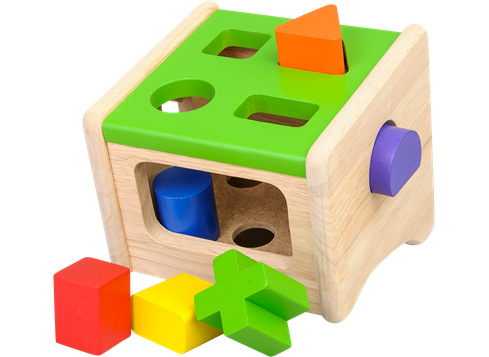
\includegraphics[width=0.8\textwidth]{../img/plocklada.png}
\end{Slide}


\begin{Slide}{Vad är matchning?}
Matchning gör man då man vill jämföra ett värde mot andra värden och hitta överensstämmelse \Eng{match}.

\pause

\vspace{1em}Detta kan man t.ex. göra med nästlade if-else-satser/uttryck:

\begin{Code}
val g = scala.io.StdIn.readLine("grönsak:")
val smak = 
  if (g == "gurka") "gott!"
  else if (g == "tomat") "jättegott!"
  else if (g == "broccoli") "ganska gott..."
  else "inte gott :("

println(g + " är " + smak)
\end{Code}
\end{Slide}
\fi

\begin{Slide}{Javas switch-sats}\SlideFontSmall
De flesta C-liknande språk (men inte Scala) har en \jcode{switch}-sats som man kan använda istället för (vissa) nästlade if-else-satser: 
\javainputlisting[basicstyle=\ttfamily\SlideFontSize{5.5}{6.8}\selectfont]{../compendium/examples/match/Switch.java}

\vspace{-0.5em}Funkar bara för primitiva typer och några till (t.ex. String).
\end{Slide}

\ifkompendium\else
\begin{Slide}{Javas switch-sats utan break}\SlideFontSmall
Saknad \jcode{break}-sats ''faller igenom'' till efterföljande gren: 

\javainputlisting[basicstyle=\ttfamily\SlideFontSize{6}{7}\selectfont]{../compendium/examples/match/SwitchNoBreak.java}
En glömd \jcode{break} kan ge svårhittad bugg... 
\end{Slide}

\begin{Slide}{Javas switch-sats med glömd break}\SlideFontSmall

\vspace{-0.5em}\javainputlisting[basicstyle=\ttfamily\SlideFontSize{5.5}{6.8}\selectfont]{../compendium/examples/match/SwitchForgotBreak.java}

\vspace{-0.7em}\pause
\begin{REPL}
$ java SwitchForgotBreak 
Skriv grönsak:
gurka
gott!
gott!
\end{REPL}

\end{Slide}


\begin{Slide}{Scalas \texttt{match}-uttryck}\SlideFontSmall
Scala har ingen \code{switch}-sats men erbjuder i stället ett \code{match}-\Emph{uttryck} som är kraftfullare och ger ett värde.

\begin{Code}
val g = scala.io.StdIn.readLine("grönsak:")
val smak = g match {
  case "gurka" => "gott!"
  case "tomat" => "jättegott!"
  case "broccoli" => "ganska gott..."
  case _ => "mindre gott..."
}
println(g + " är " + smak)
\end{Code}
Och den ''faller inte igenom'' som Javas \code{switch}-sats! 
\begin{itemize}
\pause\item Varje \code{case}-gren testas var för sig i tur och ordning uppifrån och ned.
\pause\item Det som står mellan \code{case} och \code{=>} kallas ett \Emph{mönster} \Eng{pattern}
\pause\item Sista default-grenen ovan kallas \Emph{wildcard-mönster}: \code{case _ => } 
\pause\item Ovan är exempel på matchning mot \Emph{konstant-mönster}, \\ i detta fallet tre stycken strängkonstantmönster.
\pause\item Det finns många andra sätt att skriva mönster.
\end{itemize}
\end{Slide}



\begin{Slide}{Matchning med gard}
Man kan stoppa in en s.k \Emph{gard} \Eng{guard} innan pilen \code{=>} för att villkora matchningen: (notera \code{if}, parenteser behövs ej)
\begin{Code}
val g = scala.io.StdIn.readLine("grönsak:")
def f = g match {
  case "gurka" if math.random > 0.5 => "gott ibland!"
  case "tomat" => "jättegott!"
  case "broccoli" => "ganska gott..."
  case _ => "mindre gott..."
}
\end{Code}
\code{case}-grenen med gard ger bara en lyckad matchning \\ om uttrycket efter \code{if} är sant; annars provas nästa gren, etc.
\end{Slide}

\begin{Slide}{Matchning med variabelmönster}\SlideFontSmall
Om det finns ett namn efter \code{case} som börjar med liten begynnelsebokstav, blir detta namn en variabel som automatiskt binds till uttrycket före \code{match}:

\begin{Code}
val g = scala.io.StdIn.readLine("grönsak:")
def f = g match {
  case "gurka" if math.random > 0.5 => "gott ibland!"
  case "tomat" => "jättegott!"
  case "broccoli" => "ganska gott..."
  case other => "smakar bakvänt: " + other.reverse
}
\end{Code}

Ett enkelt variabelmönster, så som \\ \code{case other => ...} \\ i exemplet ovan, matchar \Emph{allt}! \\\code{other} får alltså värdet av \code{g} om \code{g} \Alert{inte} är \code{"gurka"}, \code{"tomat"}, \code{"broccoli"}.  

\end{Slide}





\begin{Slide}{Matchning med typade mönster}\SlideFontSmall
Med en typannotering efter en variabel får man ett \Emph{typat mönster} \Eng{typed pattern}. Om matchningen lyckas blir värdet \Alert{omvandlat} till den specifika typen och binds till variabeln.
\begin{Code}
def f = if (math.random < 0.5) 42 + math.random else "gurka" + math.random
def g = f match {
  case x: Double => x.round.toInt
  case s: String => s.length
}
\end{Code}
Vad har funktionen \code{f} för returtyp? \\ \pause
Matchning mot specifika typer enl. ovan används i idiomatisk Scala hellre än \code{isInstanceOf} men man kan göra motsvarande ovan med if-uttryck:
\begin{Code}
def g2 = {
  val x = f
  if (x.isInstanceOf[Double]) x.asInstanceOf[Double].round.toInt
  else if (x.isInstanceOf[String]) x.asInstanceOf[String].length
}.asInstanceOf[Int]
\end{Code}
\end{Slide}


\begin{Slide}{Konstruktormönster med case-klasser}\SlideFontSmall
En basklass med gemensamma delar och två subtyper:
\begin{Code}
trait Grönsak {
  def vikt: Int
  def ärRutten: Boolean
}
case class Gurka(vikt: Int, ärRutten: Boolean) extends Grönsak
case class Tomat(vikt: Int, ärRutten: Boolean) extends Grönsak
\end{Code}
\pause
Tack vare case-klasserna kan man använda \Emph{konstruktormönster} \Eng{constructor pattern} för att kolla vad som finns \Alert{inuti} en instans:
\begin{Code}
def testa(g: Grönsak): String = g match {
  case Gurka(v, false) => "gott, väger " + v
  case Gurka(_, true)  => "inte gott"
  case Tomat(v, r)     => (if (r) "inte " else "") + "gott, väger " + v 
  case _ => "okänd grönsak: " + g
}
\end{Code}

Konstruktormönster ''\Emph{plockar isär}'' det som matchas och binder variabler till de attribut som finns i case-klassens konstruktor.
\end{Slide}


\begin{Slide}{Plocka isär samlingar med djupa mönster}
Man kan plocka isär innehållet i en samling så här:
\begin{Code}
def visa(xs: Vector[Grönsak]): String = xs match {
  case Vector()               => "tom grönsaksvektor"
  case Vector(Gurka(v, true)) => "en rutten gurka som väger " + v
  case Vector(g)              => "exakt en grönsak: " + g
  case Vector(g1, g2)         => s"exakt två grönsaker: $g1, $g2"
  case g +: gs                => s"först en $g och sedan svansen: $gs" 
}
\end{Code}
Övning: prova ovan i REPL. Vad händer om du byter ordning på andra och tredje mönstret ovan?
\end{Slide}

\begin{Slide}{Mönstermatchning och case-objekt}
En bastyp och specifika singelobjekt av gemensam typ:
\begin{Code}
trait Färg
case object Spader  extends Färg
case object Hjärter extends Färg
case object Ruter   extends Färg
case object Klöver  extends Färg

def parallellFärg(f: Färg): Färg = f match {
  case Spader  => Klöver
  case Klöver  => Spader
  case Hjärter => Ruter
}
\end{Code}
Vilken case-gren har vi glömt? Kan kompilatorn hjälpa oss?
\pause
\begin{REPL}
scala> parallellFärg(Ruter)
scala.MatchError: Ruter (of class Ruter$)
  at .parallellFärg(<console>:18)

\end{REPL}
Runtime exception \code{:(} ~~och en bugg som kan vara svårhittad...
\end{Slide}

\begin{Slide}{Mönstermatchning och förseglade typer}
Med nyckelordet \code{sealed} får vi en kompileringsvarning \code{:)}
\begin{Code}
sealed trait Färg
case object Spader  extends Färg
case object Hjärter extends Färg
case object Ruter   extends Färg
case object Klöver  extends Färg

def parallellFärg(f: Färg): Färg = f match {
  case Spader  => Klöver
  case Klöver  => Spader
  case Hjärter => Ruter
}
\end{Code}
\begin{REPL}
// Exiting paste mode, now interpreting.

<console>:23: warning: match may not be exhaustive.
It would fail on the following input: Ruter
       def parallellFärg(f: Färg): Färg = f match {
\end{REPL}
\end{Slide}

\begin{Slide}{Stora/små begynnelsebokstäver vid matchning}
Fallgrop: att försöka matcha på värdet av en variabel som börjar med liten bokstav.
\begin{REPL}
scala> val livetsMening = 42

scala> def ärLivetsMeningBuggig(svar: Int) = svar match {
         case livetsMening => true    // lokalt namn som matchar allt!
         case _ => false
       }

scala> ärLivetsMeningBuggig(43)
res0: Boolean = true

scala> val LivetsMening = 42   // stor begynnelsebokstav

scala> def ärLivetsMening(svar: Int) = svar match {
         case LivetsMening => true    // funkar fint!
         case _ => false
       }

scala> ärLivetsMening(43)
res1: Boolean = false
\end{REPL}
\end{Slide}


\begin{Slide}{Stora/små begynnelsebokstäver vid matchning}
Ett sätt att komma runt problemet med liten begynnelsebokstav: \\
\Emph{backticks} to the rescue!
\begin{REPL}
scala> val livetsMening = 42

scala> def ärLivetsMeningBackTicks(svar: Int) = svar match {
         case `livetsMening` => true    // nu funkar det!
         case _ => false
       }

scala> ärLivetsMeningBackTicks(43)
res2: Boolean = false<
\end{REPL}
\end{Slide}


\begin{Slide}{Mönster på andra ställen än i \texttt{match}}\SlideFontSmall
Mönster i \Emph{deklarationer}:
\vspace{-0.25em}\begin{REPL}
scala> case class Point(x: Int, y: Int)

scala> val p = Point(0, 1)

scala> val Point(x, y) = p          // konstruktormönster med case-klass
x: ???
y: ???

scala> val (x, y, z) = (0, 1, 2)    // konstruktormönster med tupel
x: ???
y: ???
z: ???

\end{REPL}
Mönster i \Emph{for-satser}:
\vspace{-0.25em}\begin{REPL}
scala> val xs = for ((x, y) <- Vector((1,2), (3,4))) yield x
xs: ???
\end{REPL}

\end{Slide}

\begin{Slide}{Mönster på andra ställen än i \texttt{match}}\SlideFontSmall
Mönster i \Emph{deklarationer}:
\vspace{-0.25em}\begin{REPL}
scala> case class Point(x: Int, y: Int)

scala> val p = Point(0, 1)

scala> val Point(x, y) = p          // konstruktormönster med case-klass
x: Int = 0
y: Int = 1

scala> val (x, y, z) = (0, 1, 2)    // konstruktormönster med tupel
x: Int = 0
y: Int = 1
z: Int = 2

\end{REPL}
Mönster i \Emph{for-satser}:
\vspace{-0.25em}\begin{REPL}
scala> val xs = for ((x, y) <- Vector((1,2), (3,4))) yield x
xs: scala.collection.immutable.Vector[Int] = Vector(1, 3)
\end{REPL}
\end{Slide}

\begin{Slide}{Fördjupning om mönster}
Avancerade saker för den intresserade (ingår ej): 
\begin{itemize}
\item binda variabler till mönsterdelar med \code{@}
\item partiella funktioner
\item att skapa extraherare med \code{unapply} och \code{unapplySeq}
\end{itemize}
Fördjupning:
\begin{itemize}
\item Läs mer om mönster här:  \href{http://www.artima.com/pins1ed/case-classes-and-pattern-matching.html}{\SlideFontTiny www.artima.com/pins1ed/case-classes-and-pattern-matching.html}

\item För djupare förståelse av hur \code{case} fungerar, läs speciellt om \Emph{partiella funktioner} här: \href{http://www.artima.com/pins1ed/case-classes-and-pattern-matching.html\#15.7}{\SlideFontTiny www.artima.com/pins1ed/case-classes-and-pattern-matching.html\#15.7}

\item Läs om extractors här: \href{http://www.artima.com/pins1ed/extractors.html}{\SlideFontTiny www.artima.com/pins1ed/extractors.html}

\end{itemize} 
\end{Slide}


\begin{Slide}{Fördjupning: metoden \texttt{unapply}}\SlideFontSmall
När du deklarerar en case-klass kommer kompilatorn att \Alert{automatiskt generera en metod} med namnet \Emph{\texttt{unapply}} som kan plocka isär instansen.
\begin{REPL}
scala> case class Gurka(vikt: Int, ärRutten: Boolean)

scala> Gurka.unapply // tryck TAB två gånger för att se metodhuvudet
 case def unapply(x$0: Gurka): Option[(Int, Boolean)]
 
scala> val g = Gurka(100, false)

scala> Gurka.unapply(g)
res0: Option[(Int, Boolean)] = Some((100,false))
\end{REPL}
Vi ska snart se hur \code{Option} kan hantera värden som \Emph{eventuellt} \Alert{saknas}. \\
\pause

{\SlideFontTiny\vspace{1em}\emph{Fördjupning:} Ett anrop av metoden \code{unapply} genereras av kompilatorn vid matchning och det är det som gör att case-klasser kan användas i konstruktormönster. Man kan skapa en egna s.k. extraktorer \Eng{extractors} som funkar i matchningar (se övn. 22).}
\end{Slide}

\fi






%!TEX encoding = UTF-8 Unicode
%!TEX root = ../lect-week09.tex

%%%

\ifkompendium\else


\Subsection{Option}


\begin{Slide}{Hur hantera saknade värden?}\SlideFontSmall
Olika sätt att hantera saknade värden:
\begin{itemize}
\item Hitta på ett specialvärde: exempel -1 för icke nedtryckt sträng
\item \code{null} om \code{AnyRef}/\code{Object} (vanligt i Java, mkt ovanligt i Scala) 
\item Använd en samling och låt tom samling representera saknad värde: \\
\code{val grip = Vector(Vector(2), Vector(7), Vector(), Vector(3))}

\item \code{Option[T]} gemensam bastyp för: \\
  \code{None} som representerar \Alert{saknat värde}, och \\ \code{Some[T]} som representerar att \Emph{värde finns}
\end{itemize}
\end{Slide}

\begin{Slide}{En gemensam bastyp för ett värde som kanske saknas}\SlideFontSmall
\vspace{-0.5em}\begin{center}
\newcommand{\TextBox}[1]{\raisebox{0pt}[1em][0.5em]{#1}}
\tikzstyle{umlclass}=[rectangle, draw=black,  thick, anchor=north, text width=3cm, rectangle split, rectangle split parts = 3]
\begin{tikzpicture}[inner sep=0.5em]
\node [umlclass, rectangle split parts = 2, xshift=0cm, text width=3.5cm] (BaseType)  {
            \textit{\textbf{\centerline{\TextBox{\code{Option[A]}}}}}
            \nodepart[]{second}
            \TextBox{\code{def get: A}}\newline
            \TextBox{\code{def isEmpty: Boolean}}

        };
        
\node [umlclass, rectangle split parts = 1]  at (-2.5cm,-3.7cm) (SubType1) {
            \textbf{\centerline{\TextBox{\code{Some[A]}}}}
            % \nodepart[]{second} \TextBox{\code{val x: A}}
        };  
                
\node [umlclass, rectangle split parts = 1] at (2.5cm,-3.7cm) (SubType2)  {
            \textbf{\centerline{\TextBox{\code{None}}}}
        };        
\draw[umlarrow] (SubType1.north) -- ++(0,0.5) -| (BaseType.south);    
\draw[umlarrow] (SubType2.north) -- ++(0,0.5) -| (BaseType.south);            
\end{tikzpicture}
\end{center}
\end{Slide}


\begin{Slide}{Option för hantering av ev. saknade värden}\SlideFontSmall
Alla vill inte berätta för Facebook vad de har för kön. \\ Förbättra Facebooks kod med ett litet Scala-program:
\begin{Code}
trait Gender
case object Male   extends Gender
case object Female extends Gender

case class Person(name: String, gender: Option[Gender])
\end{Code}
\begin{REPL}
scala> val p1 = Person("Björn",  Some(Male))
scala> val p2 = Person("Sandra", Some(Female))
scala> val p3 = Person("Andro",  None)
scala> val g2 = p2.gender
scala> def show(g: Option[Gender]): String = g match {
         case Some(x) => x.toString
         case None    => "unknown"
       }
scala> show(g2)
scala> show(p3.gender)
scala> val ps = Vector(p1,p2,p3)
scala> ps.map(_.gender).map(show)
\end{REPL}
\end{Slide}

\begin{Slide}{Några smidiga metoder på \code{Option}}
getOrElse

map

foreach

isEmpty
\end{Slide}


\begin{Slide}{Några samlingsmetoder som ger en \code{Option}}
get på Map

headOption på Vector

find på Seq
\end{Slide}



\fi



%!TEX encoding = UTF-8 Unicode
%!TEX root = ../lect-week09.tex

%%%

\ifkompendium\else
\Subsection{Implementera \texttt{equals} med \texttt{match}}
\fi












%!TEX encoding = UTF-8 Unicode
%!TEX root = ../lect-week09.tex

%%%


%\begin{Slide}{TODO: Begrepp att förklara}
%  Tänk igenom ordningen:
%  \begin{itemize}
%    \item java switch, scala match ... 
%  \end{itemize}
%\end{Slide}
%
%
%\begin{Slide}{Undantag}
%
%\begin{Code}
%try
%catch
%\end{Code}
%\end{Slide}














\Lecture{10}{Matriser, typparametrar}
%!TEX encoding = UTF-8 Unicode
%!TEX root = ../lect-week10.tex

%%%

\ifkompendium\else

\Subsection{Veckans labb: \texttt{maze}}
\begin{Slide}{Veckans labb: \texttt{maze}}\SlideFontSmall
Grunduppgift:
\begin{itemize}
\item Implementera en algoritm som hittar ut ur en labyrint.

\item En labyrint representeras av en \Emph{matris}, \\närmare bestämt en \Emph{vektor av vektorer} med  \Alert{booelska} värden: \\ \code{Vector[Vector[Boolean]]} 

\pause Där de två olika sanningsvärdena representerar följande:
\begin{itemize}\SlideFontSmall
\item \code{true} om det \Emph{finns en vägg} på en viss plats i matrisen
\item \code{false} om det \Alert{inte} finns en vägg på en viss plats i matrisen 

\end{itemize}
\pause
\item Använd enkel idé (som inte ger kortaste vägen): \\ Behåll vänster hand i kontakt med väggen och gå tills du når utgången.

\item Vad krävs av labyrinten för att detta ska fungera?  
\end{itemize}
\pause Extrauppgift:
\begin{itemize}
\item Generera slumpmässig labyrint 
\item Algoritmen (\emph{Prims algoritm}) är given i pseudokod
\end{itemize}

\end{Slide}

\begin{Slide}{Labyrint som booelsk matris}
\includegraphics[width=1.0\textwidth]{../img/w09-lab/MazeAndMatrix.jpg}
\end{Slide}

\begin{Slide}{Slumpmässig labyrint}
\includegraphics[width=0.68\textwidth]{../img/w09-lab/RandomMaze.jpg}
\end{Slide}

\Subsection{Matriser}

\begin{Slide}{Vad är en matris?}\SlideFontSmall
\begin{multicols}{2}
\begin{itemize}
\item En \Emph{matris} inom \Alert{matematiken} innehåller \Emph{rader} med lika många tal och \Emph{kolumner} med lika många tal. 

\item En matris av dimension $m\times{}n$ har $m \cdot n$ stycken element. 

\end{itemize}

\columnbreak
\begin{itemize}
\item En matris $M_{2,5}$ ritas inom matematiken ofta så här:
\end{itemize}
\[
M=
  \begin{pmatrix}
    5 & 2 & 42 & 4 & 5 \\
    3 & 4 & 18 & 6 & 7
  \end{pmatrix}
\]

\begin{itemize}
\pause
\item Indexering inom matematiken sker från 1 (men oftast från 0 i datorprogram).

\item Vad har talet 42 för index i matrisen M ovan?
\end{itemize}
\end{multicols}
\end{Slide}

\begin{Slide}{En matris med array av arrayer}
Inom programmering används ordet \Emph{matris} ofta för att beteckna en \Alert{nästlade struktur} i två dimensioner, till exempel en instans av typen \code{Array[Array[Int]]}
\begin{REPL}
scala> val xss = Array(Array(5,2,42,4,5),Array(3,4,18,6,7))
xss: Array[Array[Int]] = Array(Array(5, 2, 42, 4, 5), Array(3, 4, 18, 6, 7))
\end{REPL}
\pause
Man indexerar i en nästlad sekvens med upprepad \code{apply}:
\begin{REPL}
scala> xss(0)(2)
res0: ???                   // Vad är typ och värde?

scala> xss.apply(0).apply(2)
res1: ???                   // Vad är typ och värde?

scala> xss(0)
res2: ???                   // Vad är typ och värde?
\end{REPL}

\end{Slide}

\begin{Slide}{En matris med array av arrayer}
Inom programmering används ordet \Emph{matris} ofta för att beteckna en \Alert{nästlade struktur} i två dimensioner, till exempel en instans av typen \code{Array[Array[Int]]}
\begin{REPL}
scala> val xss = Array(Array(5,2,42,4,5),Array(3,4,18,6,7))
xss: Array[Array[Int]] = Array(Array(5, 2, 42, 4, 5), Array(3, 4, 18, 6, 7))
\end{REPL}

Man indexerar i en nästlad sekvens med upprepad \code{apply}:
\begin{REPL}
scala> xss(0)(2)
res0: Int = 42

scala> xss.apply(0).apply(2)
res1: Int = 42

scala> xss(0)
res2: Array[Int] = Array(5, 2, 42, 4, 5)
\end{REPL}
\end{Slide}

\begin{Slide}{Uppdatering av en förändringsbar nästlad struktur}
Man kan förändra en array av arrayer ''på plats'' med tilldelning:
\begin{REPL}
scala> val xss = Array(Array(5,2,42,4,5),Array(3,4,18,6,7))

scala> xss(0)(0) = 100

scala> xss
res0: ???

scala> xss(0)(2) = xss(0)(2) - 1

scala> xss
res1: ???

scala> xss(1) = Array.fill(5)(-1)

scala> xss
res2: ???
\end{REPL}
\end{Slide}

\begin{Slide}{Uppdatering av en förändringsbar nästlad struktur}
Man kan förändra en array av arrayer ''på plats'' med tilldelning:
\begin{REPL}
scala> val xss = Array(Array(5,2,42,4,5),Array(3,4,18,6,7))

scala> xss(0)(0) = 100

scala> xss
res0: Array[Array[Int]]=Array(Array(100, 2, 42, 4, 5), Array(3, 4, 18, 6, 7))

scala> xss(0)(2) = xss(0)(2) - 1

scala> xss
res1: Array[Array[Int]]=Array(Array(100, 2, 41, 4, 5), Array(3, 4, 18, 6, 7))

scala> xss(1) = Array.fill(5)(-1)

scala> xss
res2: Array[Array[Int]]=Array(Array(100, 2, 41, 4, 5), Array(-1,-1,-1,-1,-1))
\end{REPL}
\end{Slide}

\begin{Slide}{Några olika sätt att skapa förändringsbara matriser}\SlideFontSmall
Det jobbiga, primitiva sättet:
\begin{REPL}
scala> val xs = new Array[Array[Int]](2)
xs: Array[Array[Int]] = Array(null, null)

scala> for (i <- xs.indices) {xs(i) = new Array[Int](5)}

scala> xs
res0: Array[Array[Int]] = Array(Array(0, 0, 0, 0, 0), Array(0, 0, 0, 0, 0))

scala> println(xs)
[[I@196a99d0
\end{REPL}
Enklare sätt:
\begin{REPL}
scala> val xs = Array.ofDim[Int](2,5)
xs: Array[Array[Int]] = Array(Array(0, 0, 0, 0, 0), Array(0, 0, 0, 0, 0))
\end{REPL}
Enklare och tydligare sätt, där initialvärdet anges explicit:
\begin{REPL}
scala> Array.fill(2,5)(0)
res37: Array[Array[Int]] = Array(Array(0, 0, 0, 0, 0), Array(0, 0, 0, 0, 0))
\end{REPL}

\end{Slide}

\begin{Slide}{Exempel på skapande av oföränderlig nästlad struktur}\SlideFontSmall
Om du kan beräkna initialvärde direkt, använd \code{Vector.fill}:\\
{\SlideFontTiny\code{def fill[A](n1: Int, n2: Int)(elem: => A): Vector[Vector[A]]}}
\begin{REPL}
scala> Vector.fill(2,5)(scala.util.Random.nextInt(6) + 1)
res0: 
  typ???
  värde???

\end{REPL}
Om du kan beräkna initialvärde ur index, använd \code{Vector.tabulate}:\\
{\SlideFontTiny\code{def tabulate[A](n1: Int, n2: Int)(f: (Int, Int) => A): Vector[Vector[A]]}}
\begin{REPL}
scala> Vector.tabulate(5,2)((x,y) => x + y + 1)
res1: 
  typ???
  värde???

\end{REPL}
\end{Slide}

\begin{Slide}{Exempel på skapande av oföränderlig nästlad struktur}\SlideFontSmall
Om du kan beräkna initialvärde direkt, använd \code{Vector.fill}:\\
{\SlideFontTiny\code{def fill[A](n1: Int, n2: Int)(elem: => A): Vector[Vector[A]]}}
\begin{REPL}
scala> Vector.fill(2,5)(scala.util.Random.nextInt(6) + 1)
res0: 
  scala.collection.immutable.Vector[scala.collection.immutable.Vector[Int]] = 
  Vector(Vector(1, 2, 6, 2, 1), Vector(1, 4, 3, 3, 2))

\end{REPL}
Om du kan beräkna initialvärde ur index, använd \code{Vector.tabulate}:\\
{\SlideFontTiny\code{def tabulate[A](n1: Int, n2: Int)(f: (Int, Int) => A): Vector[Vector[A]]}}
\begin{REPL}
scala> Vector.tabulate(5,2)((x,y) => x + y + 1)
res1: 
  scala.collection.immutable.Vector[scala.collection.immutable.Vector[Int]] = 
  Vector(Vector(1,2), Vector(2,3), Vector(3,4), Vector(4,5), Vector(5,	6))

\end{REPL}
\end{Slide}



\begin{Slide}{Uppdatering av en oföränderlig nästlad struktur}\SlideFontSmall
Uppdatering av endimensionell struktur med \code{xs.updated}:\\
{\SlideFontTiny\code{def updated[A](index: Int, elem: A): Vector[A]} }
\begin{REPL}
scala> var xs = Vector.tabulate(5)(x => x + 1)
xs: typ??? = värde???

scala> xs = xs.updated(1, 42)
xs: typ??? = värde???
\end{REPL}

Uppdatering av nästlad struktur i två dimensioner:
\begin{REPL}
scala> var xss = Vector.tabulate(2, 5)((x,y) => x + y + 1)
xss: 
  typ??? =
  värde???

scala> xss = xss.updated(0, xss(0).updated(1, 42))
xss: 
  typ??? =
  värde???
\end{REPL}

\end{Slide}



\begin{Slide}{Uppdatering av en oföränderlig nästlad struktur}\SlideFontSmall
Uppdatering av endimensionell struktur med \code{xs.updated}:\\
{\SlideFontTiny\code{def updated[A](index: Int, elem: A): Vector[A]} }
\begin{REPL}
scala> var xs = Vector.tabulate(5)(x => x + 1)
xs: scala.collection.immutable.Vector[Int] = Vector(1, 2, 3, 4, 5)

scala> xs = xs.updated(1, 42)
xs: scala.collection.immutable.Vector[Int] = Vector(1, 42, 3, 4, 5)
\end{REPL}

Uppdatering av nästlad struktur i två dimensioner:
\begin{REPL}
scala> var xss = Vector.tabulate(2, 5)((x,y) => x + y + 1)
xss: 
  scala.collection.immutable.Vector[scala.collection.immutable.Vector[Int]] = 
  Vector(Vector(1, 2, 3, 4, 5), Vector(2, 3, 4, 5, 6))

scala> xss = xss.updated(0, xss(0).updated(1, 42))
xss: 
  scala.collection.immutable.Vector[scala.collection.immutable.Vector[Int]] = 
  Vector(Vector(1, 42, 3, 4, 5), Vector(2, 3, 4, 5, 6))
\end{REPL}

\end{Slide}


\begin{Slide}{Iterera över nästlad struktur: for-sats}\SlideFontSmall
Iterera med nästlad for-sats:
\begin{REPL}
scala> val xss = Vector.tabulate(2,5)((x,y) => x + y + 1)

scala> for (???) { 
         for (???) {
           print(xss(i)(j) + " ")
         }
         println
       }

1 2 3 4 5 
2 3 4 5 6 
\end{REPL}
\end{Slide}

\begin{Slide}{Iterera över nästlad struktur: for-sats}\SlideFontSmall
Iterera med nästlad for-sats:
\begin{REPL}
scala> val xss = Vector.tabulate(2,5)((x,y) => x + y + 1)

scala> for (i <- xss.indices) { 
         for (j <- xss(i).indices) {
           print(xss(i)(j) + " ")
         }
         println
       }

1 2 3 4 5 
2 3 4 5 6 
\end{REPL}
\end{Slide}


\begin{Slide}{Övningsexempel: Yatzy}\SlideFontSmall
Skapa en funktion \code{roll} som ger utfallet av n st tärningskast:
\begin{REPL}
scala> import scala.util.Random

scala> def roll(n: Int): Vector[Int] = ???
\end{REPL}

Skapa en funktion \code{isYatzy} som ger \code{true} om alla utfall är lika:
\begin{REPL}
scala> def isYatzy(xs: Vector[Int]): Boolean = ???
\end{REPL}
Du kan anta att xs.length > 0\\
Tips: använd metoden xs.forall: \\
\code{def forall[A](p: A => Boolean): Boolean }
\end{Slide}


\begin{Slide}{Övningsexempel: Yatzy}\SlideFontSmall
Skapa en funktion \code{roll} som ger utfallet av n st tärningskast:
\begin{REPL}
scala> import scala.util.Random

scala> def roll(n: Int): Vector[Int] = Vector.fill(n)(Random.nextInt(6) + 1)
\end{REPL}

Skapa en funktion \code{isYatzy} som ger \code{true} om alla utfall är lika:
\begin{REPL}
scala> def isYatzy(xs: Vector[Int]): Boolean = xs.forall(x => x == xs(0))
\end{REPL}
Du kan anta att xs.length > 0\\
Tips: använd metoden xs.forall: \\
\code{def forall[A](p: A => Boolean): Boolean }
\end{Slide}

\begin{Slide}{Iterera över nästlad struktur: for-sats}\SlideFontSmall
Iterera med nästlad for-sats: (vad har xss för typ?)
\begin{REPL}
scala> val xss = Vector.fill(100)(roll(5))

scala> for (???) { 
         for (???) {
           print(s"($i)($j) == " + xss(i)(j) + " ")
         }
         println(isYatzy(???))
       }

(0)(0) == 5 (0)(1) == 3 (0)(2) == 4 (0)(3) == 1 (0)(4) == 3 false
(1)(0) == 3 (1)(1) == 3 (1)(2) == 6 (1)(3) == 3 (1)(4) == 1 false
(2)(0) == 3 (2)(1) == 4 (2)(2) == 2 (2)(3) == 2 (2)(4) == 1 false
(3)(0) == 5 (3)(1) == 2 (3)(2) == 6 (3)(3) == 5 (3)(4) == 1 false
(4)(0) == 4 (4)(1) == 6 (4)(2) == 4 (4)(3) == 1 (4)(4) == 4 false
(5)(0) == 3 (5)(1) == 4 (5)(2) == 6 (5)(3) == 5 (5)(4) == 1 false
(6)(0) == 4 (6)(1) == 6 (6)(2) == 2 (6)(3) == 2 (6)(4) == 6 false
(7)(0) == 2 (7)(1) == 5 (7)(2) == 3 (7)(3) == 6 (7)(4) == 2 false
(8)(0) == 4 (8)(1) == 4 (8)(2) == 6 (8)(3) == 1 (8)(4) == 4 false
(9)(0) == 3 (9)(1) == 3 (9)(2) == 3 (9)(3) == 3 (9)(4) == 3 true
(10)(0) == 1 (10)(1) == 2 (10)(2) == 4 (10)(3) == 3 (10)(4) == 3 false
(11)(0) == 6 (11)(1) == 5 (11)(2) == 4 (11)(3) == 1 (11)(4) == 5 false
(12)(0) == 3 (12)(1) == 6 (12)(2) == 6 (12)(3) == 4 (12)(4) == 2 false
\end{REPL}
\end{Slide}

\begin{Slide}{Iterera över nästlad struktur: for-sats}\SlideFontSmall
Iterera med nästlad for-sats: (xss är en \code{Vector[Vector[Int]]})
\begin{REPL}
scala> val xss = Vector.fill(100)(roll(5))

scala> for (i <- xss.indices) { 
         for (j <- xss(i).indices) {
           print(s"($i)($j) == " + xss(i)(j) + " ")
         }
         println(isYatzy(xss(i)))
       }

(0)(0) == 5 (0)(1) == 3 (0)(2) == 4 (0)(3) == 1 (0)(4) == 3 false
(1)(0) == 3 (1)(1) == 3 (1)(2) == 6 (1)(3) == 3 (1)(4) == 1 false
(2)(0) == 3 (2)(1) == 4 (2)(2) == 2 (2)(3) == 2 (2)(4) == 1 false
(3)(0) == 5 (3)(1) == 2 (3)(2) == 6 (3)(3) == 5 (3)(4) == 1 false
(4)(0) == 4 (4)(1) == 6 (4)(2) == 4 (4)(3) == 1 (4)(4) == 4 false
(5)(0) == 3 (5)(1) == 4 (5)(2) == 6 (5)(3) == 5 (5)(4) == 1 false
(6)(0) == 4 (6)(1) == 6 (6)(2) == 2 (6)(3) == 2 (6)(4) == 6 false
(7)(0) == 2 (7)(1) == 5 (7)(2) == 3 (7)(3) == 6 (7)(4) == 2 false
(8)(0) == 4 (8)(1) == 4 (8)(2) == 6 (8)(3) == 1 (8)(4) == 4 false
(9)(0) == 3 (9)(1) == 3 (9)(2) == 3 (9)(3) == 3 (9)(4) == 3 true
(10)(0) == 1 (10)(1) == 2 (10)(2) == 4 (10)(3) == 3 (10)(4) == 3 false
(11)(0) == 6 (11)(1) == 5 (11)(2) == 4 (11)(3) == 1 (11)(4) == 5 false
(12)(0) == 3 (12)(1) == 6 (12)(2) == 6 (12)(3) == 4 (12)(4) == 2 false
\end{REPL}
\end{Slide}


\begin{Slide}{Iterera över nästlad struktur med nästlad foreach}\SlideFontSmall
Iterera med nästlad foreach-sats:
\begin{REPL}
scala> val xss = Vector.tabulate(2,5)((x,y) => x + y + 1)

xss.foreach{ xs => ??? ; println }

1 2 3 4 5 
2 3 4 5 6 
\end{REPL}
\end{Slide}


\begin{Slide}{Iterera över nästlad struktur med nästlad foreach}\SlideFontSmall
Iterera med nästlad foreach-sats:
\begin{REPL}
scala> val xss = Vector.tabulate(2,5)((x,y) => x + y + 1)

xss.foreach{ xs => xs.foreach{ x => print(x + " ") }; println }

1 2 3 4 5 
2 3 4 5 6 
\end{REPL}
\end{Slide}


\begin{Slide}{Nästlade for-uttryck}\SlideFontSmall
Iterera med \Emph{nästlad for-yield}:\\
%Statisk typ: \code{IndexedSeq[IndexedSeq[[Int]]} \\
%Dynamisk typ: \code{Vector[Vector[[Int]]}
 
\begin{REPL}
scala> val xss = for (i <- 1 to 2) yield { 
                   for (j <- 1 to 5) yield i + j + 1
                 }
xss: 
  scala.collection.immutable.IndexedSeq[
    scala.collection.immutable.IndexedSeq[Int]] = 
      ???

\end{REPL}
Om man skriver så här får man en endimensionell struktur:
\begin{REPL}
scala> val xs = for (i <- 1 to 2; j <- 1 to 5) yield i + j + 1
xs: 
  scala.collection.immutable.IndexedSeq[Int] = 
    ???

\end{REPL}
\end{Slide}

\begin{Slide}{Nästlade for-uttryck}\SlideFontSmall
Iterera med \Emph{nästlad for-yield}:\\
\begin{REPL}
scala> val xss = for (i <- 1 to 2) yield { 
                   for (j <- 1 to 5) yield i + j + 1
                 }
xss: 
  scala.collection.immutable.IndexedSeq[
    scala.collection.immutable.IndexedSeq[Int]] = 
      Vector(Vector(3, 4, 5, 6, 7), Vector(4, 5, 6, 7, 8))

\end{REPL}
Om man skriver så här får man en endimensionell struktur:
\begin{REPL}
scala> val xs = for (i <- 1 to 2; j <- 1 to 5) yield i + j + 1
xs: 
  scala.collection.immutable.IndexedSeq[Int] = 
    Vector(3, 4, 5, 6, 7, 4, 5, 6, 7, 8)

\end{REPL}
\end{Slide}



\begin{Slide}{Nästlade map-uttryck}\SlideFontSmall
Iterera med \Emph{nästlade map-uttryck}:\\
\begin{REPL}
scala> val xss = (1 to 2).map(i => (1 to 5).map(j => i + j + 1))
xss: 
  scala.collection.immutable.IndexedSeq[
    scala.collection.immutable.IndexedSeq[Int]] = 
      ???
\end{REPL}
\end{Slide}

\begin{Slide}{Nästlade map-uttryck}\SlideFontSmall
Iterera med \Emph{nästlade map-uttryck}:\\
\begin{REPL}
scala> val xss = (1 to 2).map(i => (1 to 5).map(j => i + j + 1))
xss: 
  scala.collection.immutable.IndexedSeq[
    scala.collection.immutable.IndexedSeq[Int]] = 
      Vector(Vector(3, 4, 5, 6, 7), Vector(4, 5, 6, 7, 8))
\end{REPL}
\end{Slide}




\begin{Slide}{Matris som Array med Array med heltal i Java}\SlideFontTiny
\begin{CodeSmall}[language=Java]
public class ArrayMatrix {

    public static void showMatrix(int[][] m){
        System.out.println("\n--- showMatrix ---");
        for (int row = 0; row < m.length; row++){
            for (int col = 0; col < m[row].length; col++) {
                System.out.print("[" + row + "]");
                System.out.print("[" + col + "] = ");
                System.out.print(m[row][col] + "; ");
            }
            System.out.println();
        }
    }
    
    public static void main(String[] args) {
        int[][] xss = new int[10][5];
        showMatrix(xss);
    }
}
\end{CodeSmall}
\pause
Övning: skriv en metod \code{fillRnd} som fyller en heltalsmatris med slumptal 1 till n: 
\pause
\jcode|public static void fillRnd(int[][] m, int n){ /* ??? */ }| \\
\pause
Tips: använd en nästlad for-sats och: \\ 
\jcode{(int) (Math.random * n + 1)   // (int) motsvarar Scalas asInstanceOf[Int]}

\end{Slide}

\begin{Slide}{Om veckans övningar}\SlideFontSmall
\begin{itemize}
\item Träna på att iterera i nästlade strukurer

\item Fortsätt jobba med Yatzy-exemplet

\item Övning 2f) ger träning i att skapa en \Emph{imperativ} algoritm: \\ 
lös \code{isYatzy} med \code{while}-sats (kunde varit del av en tenta...)

\item Extrauppgiften 7 är en bra träning på matriser där du ska bygga ett enkelt yatzy-spel i terminalen (kunde varit del av en tenta...)

\item Uppgift 3 är en förberedelse inför nästa veckas labb: \code{survey} då vi ska analysera enkäter och kombinera matriser \& registrering \& sortering.

\end{itemize}
\end{Slide}

\begin{Slide}{Grunduppgift 3, utgör början på labb \code{survey}}\SlideFontSmall

\begin{ScalaSpec}{Table}
object Table {
  /** Creates a new Table from fileName with columns split by sep */
  def fromFile(fileName: String, separator: Char = ';'): Table = ???
}
case class Table(
  data: Vector[Vector[String]], 
  headings: Vector[String], 
  sep: String){
  /** A 2-tuple with (number of rows, number of columns) in data */
  val dim: (Int, Int) = ???

  /** The element in row r an column c of data, counting from 0 */
  def apply(r: Int, c: Int): String = ???

  /** The row-vector r in data, counting from 0 */
  def row(r: Int): Vector[String]= ???

  /** The column-vector c in data, counting from 0 */
  def col(c: Int): Vector[String] = ???

  /** A map from heading to index counting from 0 */
  lazy val indexOfHeading: Map[String, Int] = ???

  /** The column-vector with heading h in data */
  def col(h: String): Vector[String] = ???

  /** A vector with the distinct, sorted values of col with heading h */ 
  def values(h: String): Vector[String] = ???

  /** Headings and data with columns separated by sep */
  override lazy val toString: String = ???
}
\end{ScalaSpec}
\end{Slide}


\begin{Slide}{Fördjupningsuppgift 8: skapa en generisk matris-klass}\SlideFontSmall
\vspace{-0.7em}
\begin{Code}[basicstyle=\SlideFontSize{6}{6.8}\ttfamily\selectfont]
case class Matrix[T](data: Vector[Vector[T]]){

  def foreachRowCol(f: (Int, Int, T) => Unit): Unit = 
    for (r <- data.indices) {
      for (c <- data(r).indices) {
        f(r, c, data(r)(c))
      }
    }

  def map[U](f: T => U): Matrix[U] = Matrix(data.map(_.map(f)))

  /** The element at row r and column c */
  def apply(r: Int, c: Int): T = ???

  /** Gives Some[T](element) at index (r, c) if within index bounds, else None */
  def get(r: Int, c: Int): Option[T] = ???

  /** The row vector of row r */ 
  def row(r: Int): Vector[T] = ???

  /** The column vector of column c */ 
  def col(c: Int): Vector[T] = ???

  /** A new Matrix with element at row r and col c updated */
  def updated(r: Int, c: Int, value: T): Matrix[T] = ???
}
object Matrix {
  def fill[T](rowSize: Int, colSize: Int)(init: T): Matrix[T] = 
    new Matrix(Vector.fill(rowSize)(Vector.fill(colSize)(init)))  
}
\end{Code}
\end{Slide}


\fi












%!TEX encoding = UTF-8 Unicode
%!TEX root = ../lect-week10.tex

\ifkompendium\else

\Subsection{Typparametrar}

\begin{Slide}{Vad är en typparameter?}\SlideFontSmall
\begin{itemize}
\item En \Emph{typparameter} gör det möjligt att ge ett \Emph{typargument}
\item En \Emph{fri} typparameter kan bindas till vilken typ som helst 
\item Bindingen sker vid \Alert{kompileringstid}
\item En typparameter är \Emph{fri} om den \Alert{inte} fått något värde i omslutande deklarationer, annars \Emph{bunden}.
\end{itemize}
Exempel: \Emph{generisk} metod:
\begin{Code}
def tnirp[A](x: A):Unit = println(x.toString.reverse)
\end{Code}
\pause
Exempel: \Emph{generisk} klass:
\begin{Code}
class Cell[A](var value: A){
  override def toString = s"Cell($value)"
  def concat(x: A): Cell[String] = new Cell(value.toString + x)   // A bunden
  def tnirp[B](x: B): Unit = println(x.toString.reverse)          // B fri
} 
\end{Code}
\pause
\begin{itemize}
\item \Alert{Skuggning kan förekomma}: Om \code{tnirp} i \code{Cell} hade använt namnet A på sin typparameter hade den \Emph{skuggat} klassens typparameter och blivit en ny fri typparameter.
\end{itemize}

\end{Slide}

\begin{Slide}{Exempel: Generisk funktion}
Vad händer här?
\begin{REPL}

scala> def skrikBaklänges(x: T): String = x.toString.toUpperCase.reverse
???



scala> def skrikBaklänges[T](x: T): String = x.toString.toUpperCase.reverse

scala> skrikBaklänges("gurka är gott")
res0: ???

\end{REPL}
\end{Slide}

\begin{Slide}{Exempel: Generisk funktion}
Vad händer här?
\begin{REPL}

scala> def skrikBaklänges(x: T): String = x.toString.toUpperCase.reverse
<console>:11: error: not found: type T
       def skrikBaklänges(x: T): String = x.toString.toUpperCase.reverse
                             ^

scala> def skrikBaklänges[T](x: T): String = x.toString.toUpperCase.reverse

scala> skrikBaklänges("gurka är gott")
res0: ???
\end{REPL}
\end{Slide}

\begin{Slide}{Exempel: Generisk funktion}
Vad händer här?
\begin{REPL}

scala> def skrikBaklänges(x: T): String = x.toString.toUpperCase.reverse
<console>:11: error: not found: type T
       def skrikBaklänges(x: T): String = x.toString.toUpperCase.reverse
                             ^

scala> def skrikBaklänges[T](x: T): String = x.toString.toUpperCase.reverse

scala> skrikBaklänges("gurka är gott")
res0: String = TTOG RÄ AKRUG
\end{REPL}
\end{Slide}


\begin{Slide}{Exempel: Generisk case-klass}
\vspace{-0.5em}\begin{REPL}
scala> def skrikBaklänges[T](x: T): String = x.toString.toUpperCase.reverse

scala> case class Grönsak(whatever: A)
???
 
 
scala> case class Grönsak[A](whatever: A)

scala> Grönsak("gurka")
res1: ???

scala> skrikBaklänges(Grönsak(42))
res2: ???

scala> Grönsak[Int](42)
res3: ???

scala> Grönsak[String](42)
???



                       ^
\end{REPL}
\end{Slide}

\begin{Slide}{Exempel: Generisk case-klass}
\vspace{-0.5em}\begin{REPL}
scala> def skrikBaklänges[T](x: T): String = x.toString.toUpperCase.reverse

scala> case class Grönsak(whatever: A)
<console>:11: error: not found: type A
       case class Grönsak(whatever: A)
                                    ^
scala> case class Grönsak[A](whatever: A)

scala> Grönsak("gurka")
res1: Grönsak[String] = Grönsak(gurka)

scala> skrikBaklänges(Grönsak(42))
res2: String = )24(KASNÖRG

scala> Grönsak[Int](42)
res3: Grönsak[Int] = Grönsak(42)

scala> Grönsak[String](42)
<console>:14: error: type mismatch;
 found   : Int(42)
 required: String
       Grönsak[String](42)
                       ^
\end{REPL}
\end{Slide}

\begin{Slide}{Fallgrop: likhet av array}
\begin{REPL}
scala> Vector.fill(5)(42) == Vector.fill(5)(42)
res0: ???

scala> Array.fill(5)(42) == Array.fill(5)(42)
res1: ???
\end{REPL}
\end{Slide}


\begin{Slide}{Fallgrop: likhet av array}
\begin{REPL}
scala> Vector.fill(5)(42) == Vector.fill(5)(42)
res0: Boolean = true

scala> Array.fill(5)(42) == Array.fill(5)(42)
res1: Boolean = false  // AAAARRGH!!! :(
\end{REPL}
Primitiva arrayer har en equals-metod som ger referenslikhet, \Alert{inte} innehållslikhet.
\end{Slide}

\begin{Slide}{Kolla likhet av array-matris med nästlad while}
\begin{REPL}
scala> def isEqual(xss: Array[Array[Int]], yss: Array[Array[Int]]) = {
         var i = 0
         var allEqual = true
         while (???) {
           var j = 0
           while (???) {
             if (xss(i)(j) != yss(i)(j)) ???
             j += 1
           }
           i += 1
         }
         allEqual
       }

scala> val (xss, yss) = (Array.fill(5,2)(42), Array.fill(5,2)(42))

scala> isEqual(xss, yss)

scala> yss(4)(1) = 0

scala> isEqual(xss, yss)
\end{REPL}
\end{Slide}



\begin{Slide}{Kolla likhet av array-matris med nästlad while}
\begin{REPL}
scala> def isEqual(xss: Array[Array[Int]], yss: Array[Array[Int]]) = {
         var i = 0
         var allEqual = true
         while (i < xss.length && allEqual) {
           var j = 0
           while (j < xss(i).length && allEqual) {
             if (xss(i)(j) != yss(i)(j)) allEqual = false
             j += 1
           }
           i += 1
         }
         allEqual
       }

scala> val (xss, yss) = (Array.fill(5,2)(42), Array.fill(5,2)(42))

scala> isEqual(xss, yss)

scala> yss(4)(1) = 0

scala> isEqual(xss, yss)
\end{REPL}
\end{Slide}


\begin{Slide}{Fördjupning: Fallgrop typradering \Eng{type erasure}}\SlideFontSmall
Informationen om typerna i typparametrar raderas innan kodgenerering av prestandaskäl och \Alert{typinformationen finns ej vid runtime}.
\vspace{-0.25em}\begin{REPL}
scala> val xs = Vector(1,2,3)
xs: scala.collection.immutable.Vector[Int] = Vector(1, 2, 3)

scala> val ys = xs.map(_.toDouble)
ys: scala.collection.immutable.Vector[Double] = Vector(1.0, 2.0, 3.0)

scala> def hasDoubles[T](xs: Vector[T]): Boolean = xs match {
         case _: Vector[Int] => false
         case _: Vector[Double] => true
       }

<console>:13: warning: ???


                        ^
<console>:14: warning: ???


                        ^
<console>:14: warning: ???
\end{REPL}
\end{Slide}


\begin{Slide}{Fördjupning: Fallgrop typradering \Eng{type erasure}}\SlideFontSmall
Informationen om typerna i typparametrar raderas innan kodgenerering av prestandaskäl och \Alert{typinformationen finns ej vid runtime}.
\vspace{-0.25em}\begin{REPL}
scala> val xs = Vector(1,2,3)
xs: scala.collection.immutable.Vector[Int] = Vector(1, 2, 3)

scala> val ys = xs.map(_.toDouble)
ys: scala.collection.immutable.Vector[Double] = Vector(1.0, 2.0, 3.0)

scala> def hasDoubles[T](xs: Vector[T]): Boolean = xs match {
         case _: Vector[Int] => false
         case _: Vector[Double] => true
       }

<console>:13: warning: non-variable type argument Int in type pattern scala.collection.immutable.Vector[Int]
is unchecked since it is eliminated by erasure
                case _: Vector[Int] => false
                        ^
<console>:14: warning: non-variable type argument Double in type pattern scala.collection.immutable.Vector[Int]
is unchecked since it is eliminated by erasure
                case _: Vector[Double] => true
                        ^
<console>:14: warning: unreachable code: case _: Vector[Double] => true
\end{REPL}
\end{Slide}

\begin{Slide}{Fördjupning: Dynamisk typtest vid typradering}\SlideFontSmall
Typtest vid körtid med nästlad matchning:
\begin{REPL}
scala> def hasDoubles2[T](xs: Vector[T]): Boolean = xs match {
         case x +: xs => x match { 
           case _: Double => true
           case _ => false
         }  
         case _ => false
       }

scala> hasDoubles2(Vector(1.0))    // funkar!
\end{REPL}

Typtest vid körtid med match och gard med \code{isInstanceOf}:
\begin{REPL}
       
scala> def hasDoubles3[T](xs: Vector[T]): Boolean = xs match {
         case x +: xs if x.isInstanceOf[Double] => true
         case _ => false
       }

scala> hasDoubles3(Vector(1.0))    // funkar!
       
       
\end{REPL}
\end{Slide}


\begin{Slide}{Typparametrar på tentan?}
\begin{itemize}
\item Det ingår att kunna använda färdiga generiska strukturer med specifik typer, t.ex. \code{Vector[Int]}

\item Det ingår att kunna skapa strukturer med specifika typparametrar, t.ex. en case-klass som tar en vektor med en specifik typ:\\
\code{case class X(x: Vector[Int])}



\item Det ingår \Alert{inte} på tentan att kunna skapa generiska metoder eller klasser, t.ex.: \\
\code{def f[T](x: Vector[T]): Vector[T] = ???} \\
Mer om generiska strukturer fortsättningskursen!
\end{itemize}
\end{Slide}

\fi








\Lecture{11}{Sökning, sortering}
%!TEX encoding = UTF-8 Unicode
%!TEX root = ../lect-week11.tex

%%%

\ifkompendium\else

\Subsection{Veckans labb: \texttt{survey2}}
\begin{Slide}{Veckans labb: \texttt{survey2}}\SlideFontTiny
\begin{minipage}{0.65\textwidth}
Nya version 2 av labben är enklare och kräver ej att du implementerar parsning av \code{args}. Välj själv vilken du gör.

\vspace{0.5em}
\Emph{Förberedelse:}
\begin{itemize}
\item Studera givna koden: {\SlideFontTiny \href{https://github.com/lunduniversity/introprog/tree/master/workspace/w10_survey2/src/main/scala/stats}{workspace/w10\_survey2}}
\item Fyll i denna enkät:
\\{\SlideFontTiny \url{https://goo.gl/forms/hC6JK2UQXVpbGECc2}} 
\end{itemize}

\Emph{Grunduppgift:}
\begin{itemize}
\item Implementera en klass \code{Table} för hantering av strängmatriser med rubrikrad från kolumnsepararade textfiler.
\item Öva på att kombinera matriser, sortering, registrering för att räkna statistik.
\item Använda inbyggda sorteringsfunktioner: \\\code{sortBy} och \code{sortWith}
\item Implementera din egen sortering ''från scratch''.
\end{itemize}
\Emph{Extrauppgift:}
\begin{itemize}
\item Implementera stapeldiagram.
\end{itemize}
\end{minipage}
\hfill\begin{minipage}{0.27\textwidth}
\centering
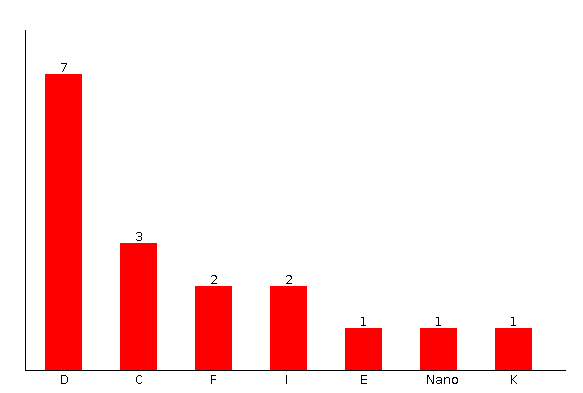
\includegraphics[width=0.9\textwidth]{../img/survey/bar}

\vspace{2em}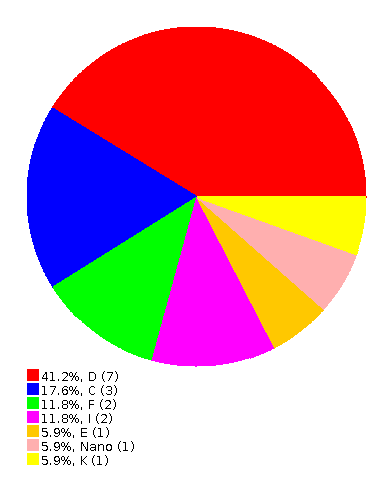
\includegraphics[width=0.7\textwidth]{../img/survey/pie}
\end{minipage}
\end{Slide}


\fi












%!TEX encoding = UTF-8 Unicode
%!TEX root = ../lect-week11.tex

%%%

\ifkompendium\else
\subsection{Repetition: Vad är en algoritm?}
\begin{Slide}{Repetition: Vad är en algoritm? }\SlideFontSmall
En \href{https://sv.wikipedia.org/wiki/Algoritm}{algoritm} är en stegvis beskrivning av hur man löser ett problem. \\ 
Exempel: MIN, Registrering, Sökning, Sortering \\
\vspace{1em}
Problemlösningsprocessens olika steg (inte nödvändigtvis i denna ordning): 
\begin{itemize}
\item identifiera (del)\Emph{problemet} och ange tydligt indata och utdata: \\ exempel MIN: indata: sekvens av heltal; utdata: minsta talet
\item Kom på en \Emph{lösningsidé}: (kan  vara mycket klurigt och svårt) \\ exempel MIN: iterera över talen och håll reda på ''minst hittills''
\item Formulera en \Emph{stegvis beskrivning} som löser problemet: \\ exempel: pseudo-kod med sekvens av instruktioner
\item Implementera en \Emph{körbar lösning} i ''riktig'' kod: \\ exempel: en Scala-metod i en klass eller i ett singelobjekt
\end{itemize}
Det krävs ofta \Emph{kreativitiet} i stegen ovan  -- även i att \Emph{känna igen} problemet!\\
Simpelt exempel: Du stöter på problemet MAX och ser likheten med MIN.\\
\vspace{0.5em}
\pause\Emph{Övning}: Diskutera hur du löser detta problem i relation till stegen ovan: \\
\emph{Att räkna antalet förekomster av olika unika ord i en textsträng.} 
\end{Slide}


\fi












%!TEX encoding = UTF-8 Unicode
%!TEX root = ../lect-week11.tex

%%%

\ifkompendium\else

\Subsection{Jämföra strängar}

\begin{Slide}{Att jämföra strängar lexikografiskt}\SlideFontSmall
\begin{REPLnonum}
scala> Array("hej","Hej","gurka").sorted
\end{REPLnonum}
\pause\vspace{-1.2em}
\begin{REPLnonum}
res0: Array[String] = Array(Hej, gurka, hej)\end{REPLnonum}
\pause
\begin{itemize}
\item Antag att vi vill lösa detta problem ''från scratch'': \\ \Emph{att sortera en sekvens med strängar} 
\item För att göra detta behöver vi lösa dessa delproblemen: 
\begin{itemize}
\item \Emph{att} \Alert{jämföra strängar}
\item \Emph{sökning i sekvenser}
\item \Emph{SWAP} (om på-plats-sortering i förändringsbar sekvens)
\end{itemize}
\item Vad betyder det att två strängar är ''lika''?

\item Vad betyder det att en sträng är ''mindre'' än en annan?
\end{itemize}
\pause {\SlideFontTiny Vi använder här strängjämförelse, sökning och sortering för att illustrera typiska \Emph{imperativa algoritmer}. \Alert{Normalt} använder man \Emph{färdiga lösningar} på dessa problem!}

\end{Slide}

\begin{Slide}{Jämföra strängar: likhet}\SlideFontSmall
Antag att vi inte kan göra \code{s1 == s2} utan bara kan jämföra strängar tecken för tecken, 
t.ex. så här: \code{s1(i) == s2(i)}. Antag också att vi inte har tillgång till annat än metoderna \code{length} och \code{apply} på strängar, samt  \code{while} och variabler av grundtyp. \Emph{Lös problemet att \emph{avgöra om två strängar är lika}.}

\pause
\begin{itemize}
\item Indata: två strängar
\item Utdata: \code{true} om lika annars \code{false}
\end{itemize}
\begin{enumerate}
\item Klura ut din lösningsidé
\item Formulera algoritmen i pseudokod
\item Implementera algoritmen i Scala: \code{def isEqual(s1: String, s2: String): Boolean} = ???
\end{enumerate}
\end{Slide}

\begin{Slide}{Algoritmexempel: stränglikhet}
Pseudokod:
\begin{Code}[H]
def isEqual(s1: String, s2: String): Boolean = {
  if (/* lika längder */) {
    var foundDiff = false
    var i = /* första index */
    while (!foundDiff && /* i inom indexgräns */) {
      if (/* tecken på plats i är olika */) foundDiff = true
      else i = /* nästa index */
    }
    !foundDiff
  } else false
}
\end{Code}
\end{Slide}

\begin{Slide}{Algoritmexempel: stränglikhet}\SlideFontSmall
\begin{Code}[H]
def isEqual(s1: String, s2: String): Boolean = {
  if (s1.length == s2.length) {
    var foundDiff = false
    var i = 0
    while (!foundDiff && i < s1.length) {
      if (s1(i) != s2(i)) foundDiff = true
      else i += 1
    }
    !foundDiff
  } else false
}
\end{Code}
\pause 
{\SlideFontTiny Fördjupning: jämför ovan med implementationen av \code{String.equals} här:
\href{http://hg.openjdk.java.net/jdk8u/jdk8u60/jdk/file/935758609767/src/share/classes/java/lang/String.java#l976}{hg.openjdk.java.net/jdk8u/jdk8u60/jdk/file/935758609767/src/share/classes/java} \\ och använd \code{timed} nedan och jämför prestanda med \code{isEqual} ovan.\\
Obs! Mät många gånger så att JVM:en optimerar din kod.}
\begin{Code}
def timed[T](block: => T): (Double, T) = { 
  val (t, res) = (System.nanoTime, block)
  ((System.nanoTime - t) / 1e9, res) 
}
\end{Code}

\end{Slide}

\begin{Slide}{Algoritmexempel: stränglikhet, prestanda}
\begin{REPL}
scala> val enMiljon = 1000000

scala> val s = Array.fill(enMiljon)('x').mkString

scala> val t = s.updated(enMiljon - 1, 'y')

scala> timed{s == t}
res42: (Double, Boolean) = (3.76459E-4,false)

scala> timed{isEqual(s,t)}
res43: (Double, Boolean) = (3.31597E-4,false)
\end{REPL}
Ovan är kört efter ''uppvärmning'' på i7-4790K CPU @ 4.00GHz \\
Skillnaden inom mätfelmarginalen!
\end{Slide}



\begin{Slide}{Jämföra strängar: ''mindre än''}\SlideFontSmall
Med \code{s1 < s2} menar vi att strängen s1 ska sorteras före strängen s2 enligt hur de enskilda tecknen är ordnade med uttrycket \code{s1(i) < s2(i)}. \\
Antag också att vi inte har tillgång till annat än metoderna \code{length} och \code{apply} på strängar, samt  \code{while} och variabler av grundtyp, samt \code{math.min}
\\\Emph{Lös problemet att \emph{avgöra om en sträng är ''mindre'' än en annan}.}\\
\begin{itemize}
\item Indata: två strängar, s1, s2
\item Utdata: \code{true} om s1 ska sorteras före s2 annars \code{false}
\end{itemize}
\begin{enumerate}
\item Klura ut din lösningsidé
\item Formulera algoritmen i pseudokod
\item Implementera algoritmen i Scala: \code{def isLessThan(s1: String, s2: String): Boolean} = ???
\end{enumerate}
\end{Slide}

\begin{Slide}{Jämföra strängar: ''mindre än''}\SlideFontSmall
Pseudokod:
\begin{Code}[H]
def isLessThan(s1: String, s2: String): Boolean = {
  
  val minLength = /* minimum av längderna på s1 och s2 */
  
  def firstDiff(s1: String, s2: String): Int = 
    /* index för första skillnaden (om de börjar lika: minLength) */

  val diffIndex = firstDiff(s1, s2)
  if (diffIndex == minLength) /* s1 är kortare än s2 */
  else /* tecknet s1(diffIndex) är mindre än tecknet s2(diffIndex) */ 
}
\end{Code}
\end{Slide}

\begin{Slide}{Jämföra strängar: ''mindre än''}\SlideFontSmall
\begin{Code}[H]
def isLessThan(s1: String, s2: String): Boolean = {

  val minLength = math.min(s1.length, s2.length)

  def firstDiff(s1: String, s2: String): Int = {
    var foundDiff = false
    var i = 0
    while (!foundDiff && i < minLength) 
      if (s1(i) != s2(i)) foundDiff = true else i += 1
    i
  }

  val diffIndex = firstDiff(s1, s2)
  if (diffIndex == minLength) s1.length < s2.length
  else s1(diffIndex) < s2(diffIndex)
}
\end{Code}
\end{Slide}

\begin{Slide}{Jämföra strängar i Java}\SlideFontTiny
\begin{itemize}
\item I Java kan man \Alert{inte} jämföra strängar med operatorerna \code{<}, \code{<=}, \code{>}, och \code{>=}

\item Dessutom ger operatorerna \code{==} och \code{!= } \emph{inte} innehålls(o)likhet utan \Alert{referens(o)likhet} \code{:(}

\item Istället \Alert{måste} man i Java använda metoderna \code{equals} och \code{compareTo} 
\\Dessa fungerar även i Scala eftersom strängar i Scala och Java är av samma typ, nämligen \code{java.lang.String}.
\pause
\item \code{s1.compareTo(s2)} ger ett heltal som är:
\begin{itemize}\SlideFontTiny
\item \code{0} om s1 och s2 har samma innehåll
\item \Alert{negativt} om s1 < s2 i lexikografiks mening, alltså s1 ska sorteras \Alert{före}
\item \Emph{positivt} om s1 > s2 i lexikografiks mening, alltså s1 ska sorteras \Emph{efter}
\end{itemize}

\pause
\item Undersök följande:
\begin{REPL}
scala> new String("hej") eq new String("hej") // motsvarar == i Java
scala> "hej".equals("hej")                    // samma som == i Scala
scala> "hej".compareTo("hej")
scala> "hej".compareTo("HEJ")         // alla stora är 'före' alla små
scala> "HEJ".compareTo("hej")
\end{REPL}
\end{itemize}

\href{http://docs.oracle.com/javase/8/docs/api/java/lang/String.html#compareTo-java.lang.String-}{docs.oracle.com/javase/8/docs/api/java/lang/String.html\#compareTo-java.lang.String-}
\end{Slide}


\begin{Slide}{Jämföra strängar i Java: exempel}\SlideFontSmall
Vad skriver detta Java-program ut?
\javainputlisting{../compendium/examples/StringEqTest.java}
\pause
\begin{REPL}
$ javac StringEqTest.java 
$ java StringEqTest 
false
true
0
\end{REPL}
\end{Slide}


\fi












%!TEX encoding = UTF-8 Unicode
%!TEX root = ../lect-week11.tex

%%%

\ifkompendium\else

\Subsection{Jämförelse Scala och Java}
\begin{Slide}{Grundläggande likheter och skillnader}\SlideFontSmall

\begin{itemize}
\item \Emph{Sökning} återkommer i många skepnader: \\ i en datastruktur, vilken det än må vara, vill man ofta kunna \\ \Emph{hitta ett element med en viss egenskap}. 

\pause
Några färdiga linjärsökningar i Scalas standardbibliotek:

\begin{REPL}
scala> Vector("gurka","tomat","broccoli").indexOf("tomat")
res0: Int = 1

scala> Vector("gurka","tomat","broccoli").indexWhere(_.contains("o"))
res1: Int = 1

scala> Vector("gurka","tomat","broccoli").find(_.contains("o"))
res2: Option[String] = Some(tomat)
\end{REPL}

\pause
\item Sökning efter ett visst index i en sekvens:

\begin{itemize}\SlideFontTiny
\item Indata: en sekvens och ett \Emph{sökkriterium}
\item Utdata: index för första eftersökta element, annars -1 
\end{itemize}

\pause
\item Två typiska varianter av sökning i en sekvens:
\begin{itemize}\SlideFontTiny
\item Linjärsökning: börja från början och sök tills ett eftersökt element är funnet
\item Binärsökning: antag sorterad sekvensen; börja i mitten, välj rätt halva ...
\end{itemize}
\end{itemize}
\end{Slide}

\Subsection{Linjärsökning}

\begin{Slide}{Linjärsökning: hitta index för elementet 42}
Skriv pseudokod för:\\ \code{def indexOf42(xs: Vector[Int]): Int = ???}
\pause
\begin{Code}
def indexOf42(xs: Vector[Int]): Int = {
  var i = /* index för första elementet */
  var found = false
  while (!found && /* index inom indexgräns */) {
    if (/* element på plats i är 42 */) found = true 
    else i = /* nästa index */
  }
  if (/* hittat */) i else -1
} 
\end{Code}
\end{Slide}

\begin{Slide}{Linjärsökning: hitta index för elementet 42}
Implementera:\\ \code{def indexOf42(xs: Vector[Int]): Int = ???}
\pause
\begin{Code}
def indexOf42(xs: Vector[Int]): Int = {
  var i = 0
  var found = false
  while (!found && i < xs.length) {
    if (xs(i) == 42) found = true 
    else i += 1
  }
  if (found) i else -1
} 
\end{Code}
\end{Slide}

\begin{Slide}{Linjärsökning: hitta index för elementet x}
Implementera:\\ \code{def indexOf(xs: Vector[Int], x: Int): Int = ???}
\pause
\begin{Code}
def indexOf(xs: Vector[Int], x: Int): Int = {
  var i = 0
  var found = false
  while (!found && i < xs.length) {
    if (xs(i) == x) found = true 
    else i += 1
  }
  if (found) i else -1
} 
\end{Code}
\end{Slide}

\begin{Slide}{Linjärsökning: hitta index för elementet p(x)}\SlideFontSmall
Implementera:\\ \code{def indexWhere(xs: Vector[Int], p: Int => Boolean): Int = ???}
\pause
\begin{Code}
def indexWhere(xs: Vector[Int], p: Int => Boolean): Int = {
  var i = 0
  var found = false
  while (!found && i < xs.length) {
    if (p(xs(i))) found = true 
    else i += 1
  }
  if (found) i else -1
} 
\end{Code}
\end{Slide}

\begin{Slide}{Linjärsökning: generalisera till godtycklig typ}\SlideFontSmall
Implementera:\\ \code{def indexWhere[T](xs: Vector[T], p: T => Boolean): Int = ???}
\pause
\begin{Code}
def indexWhere[T](xs: Vector[T], p: T => Boolean): Int = {
  var i = 0
  var found = false
  while (!found && i < xs.length) {
    if (p(xs(i))) found = true 
    else i += 1
  }
  if (found) i else -1
} 
\end{Code}
\end{Slide}

\begin{Slide}{Linjärsökning: generalisera till godtycklig typ}\SlideFontSmall
Typinferensen fungerar bättre om stegad funktion:\\ 
\code{def indexWhere[T](xs: Vector[T])(p: T => Boolean): Int}
\begin{Code}
def indexWhere[T](xs: Vector[T])(p: T => Boolean): Int = {
  var i = 0
  var found = false
  while (!found && i < xs.length) {
    if (p(xs(i))) found = true 
    else i += 1
  }
  if (found) i else -1
} 
\end{Code}
\end{Slide}


\begin{Slide}{Linjärsökning: generalisera till godtycklig sekvens}\SlideFontSmall
Implementera:\\ \code{def indexWhere[T](xs: Seq[T])(p: T => Boolean): Int = ???}
\pause
\begin{Code}
def indexWhere[T](xs: Seq[T])(p: T => Boolean): Int = {
  var i = 0
  var found = false
  while (!found && i < xs.length) {
    if (p(xs(i))) found = true 
    else i += 1
  }
  if (found) i else -1
} 
\end{Code}
\end{Slide}

\begin{Slide}{Linjärsökning: generalisera till godtycklig sekvens}\SlideFontSmall
Implementera:\\ \code{def find[T](xs: Seq[T])(p: T => Boolean): Option[T] = ???}
\pause
\begin{Code}
def find[T](xs: Seq[T])(p: T => Boolean): Option[T] = {
  var i = 0
  var found = false
  while (!found && i < xs.length) {
    if (p(xs(i))) found = true 
    else i += 1
  }
  if (found) Some(xs(i)) else None
} 
\end{Code}
\end{Slide}

\Subsection{Binärsökning}

\begin{Slide}{Binärsökning: snabbare men kräver sorterad sekvens}
\begin{REPL}[basicstyle=\color{white}\ttfamily\SlideFontSize{6.5}{8}]
scala> val enMiljon = 1000000

scala> val xs = Array.tabulate(enMiljon)(i => i + 1)   // sorterad

scala> xs(enMiljon - 1)
res0: Int = 1000000

scala> timed { xs.indexOf(enMiljon) }        // linjärsökning
res42: (Double, Int) = (0.016622994,999999)

scala> import scala.collection.Searching._  // ger tillgång till metoden search
import scala.collection.Searching._

scala> timed { xs.search(enMiljon) }        // binärsökning
res54: (Double, collection.Searching.SearchResult) = (2.45691E-4,Found(999999))

\end{REPL}
\pause
Citat från scaladoc för \code{search}:\\
''The sequence \Alert{should be sorted} before calling; otherwise, the results are \Alert{undefined.}''
\end{Slide}

\begin{Slide}{Binärsökning: lösningsidé}
\Emph{Problemlösningsidé}: Om sekvensen är sorterad kan vi utnyttja detta för en mer effektiv sökning, genom att jämföra med mittersta värdet och se om det vi söker finns före eller efter detta, och upprepa med ''halverad'' sekvens tills funnet.
\pause
\begin{itemize}\SlideFontSmall
\item \Emph{Indata}: sorterad sekvens av heltal och det eftersökta elementet
\item \Emph{Utdata}: \code{Found(index)} för det eftersökta elementet
\\ om saknas: \code{InsertionPoint(index)}
\pause
\begin{Code}
sealed trait SearchResult {
  def insertionPoint: Int
}

case class Found(foundIndex: Int) extends SearchResult {
  override def insertionPoint = foundIndex
}
  
case class InsertionPoint(insertionPoint: Int) extends SearchResult
\end{Code}
\end{itemize} 
\end{Slide}

\begin{Slide}{Binärsökning: pseudokod, iterativ lösning}
\Emph{Pseudo-kod}: iterativ lösning
\begin{Code}
def binarySearch(xs: Vector[Int])(elem: Int): SearchResult = {
  var found = false
  var (low, high) = (/* lägsta index */, /* högsta index */)
  var mid = /* något startvärde */ 
  while (!found && /* finns fler element kvar */) {
    mid = /* mittpunkten i intervallet (low, high) */
    if (xs(mid) == elem) found = true
    else if (xs(mid) < elem) /* flytta intervallets undre gräns */
    else /* flytta intervallets övre gräns" */
  }
  if (found) Found(mid)
  else InsertionPoint(low)
}
\end{Code}
\end{Slide}



\begin{Slide}{Binärsökning: implementation, iterativ lösning}
\Emph{Implementation}: iterativ lösning
\begin{Code}
def binarySearch(xs: Vector[Int])(elem: Int): SearchResult = {
  var found = false
  var (low, high) = (0, xs.length - 1)
  var mid = -1 
  while (!found && low <= high) {
    mid = (low + high) / 2
    if (xs(mid) == elem) found = true
    else if (xs(mid) < elem) low = mid + 1
    else high = mid - 1 
  }
  if (found) Found(mid) 
  else InsertionPoint(low)
}
\end{Code}
\end{Slide}

\begin{Slide}{Binärsökning: instrumentering av iterativ lösning}
\vspace{-0.5em}
\begin{CodeSmall}
def waitForEnter: Unit = scala.io.StdIn.readLine("")
def show(msg: String): Unit = {println(msg); waitForEnter}

def binarySearch(xs: Vector[Int])(elem: Int): SearchResult = {
  var found = false                         ; show(s"found = $found")
  var (low, high) = (0, xs.length - 1)      ; show(s"(low, high) = ($low, $high)")
  var mid = -1                              ; show(s"mid = $mid")
  while (!found && low <= high) {           ; show(s"while ${!found && low <= high}")
    mid = (low + high) / 2                  ; show(s"mid = $mid")
    if (xs(mid) == elem) {found = true      ; show(s"found = $found")}
    else if (xs(mid) < elem) {low = mid + 1 ; show(s"low = $low")}
    else {high = mid - 1                    ; show(s"high = $high")}
  }
  if (found) Found(mid) 
  else InsertionPoint(low)
}
\end{CodeSmall}
\vspace{-0.5em}
\begin{REPL}[basicstyle=\color{white}\ttfamily\SlideFontSize{6}{7}]
scala> binarySearch(Vector(0,1,2,3,42,5))(42)
found = false
(low, high) = (0, 5)
mid = -1
while true
mid = 2
low = 3
while true
mid = 4
found = true
res0: collection.Searching.SearchResult = Found(4)
\end{REPL}
\end{Slide}

\begin{Slide}{Binärsökning: rekursiv lösning}
\Emph{Fördjupning}: rekursiv lösning
\begin{Code}
def binarySearch(xs: Vector[Int])(elem: Int): SearchResult = {
  def loop(low: Int, high: Int): SearchResult = 
    if (low > high) InsertionPoint(low) 
    else (low + high) / 2 match {
      case mid if xs(mid) == elem => Found(mid)
      case mid if xs(mid) < elem  => loop(mid + 1, high)
      case mid                    => loop(low, mid - 1)
    }
    
  loop(0, xs.length - 1) 
}
\end{Code}
\end{Slide}


\begin{Slide}{Binärsökning: generisk rekursiv lösning}
\Emph{Fördjupning}: iterativ generisk lösning med implicit ordning
\begin{CodeSmall}
def binarySearch[T](xs: Seq[T])(elem: T)(implicit ord: Ordering[T]): SearchResult = {
  import ord._
  def loop(low: Int, high: Int): SearchResult = 
    if (low > high) InsertionPoint(low) 
    else (low + high) / 2 match {
      case mid if xs(mid) == elem => Found(mid)
      case mid if xs(mid) < elem  => loop(mid + 1, high)
      case mid                    => loop(low, mid - 1)
    }
    
  loop(0, xs.length - 1) 
}
\end{CodeSmall}
{\SlideFontSmall För den intresserade:\\Se fördjupningsuppgifter om implicita ordningar i veckans övning.}
\end{Slide}

\begin{Slide}{Tidskomplexitet, sökning}\SlideFontSmall

\Emph{Fördjupning:}\\Algoritmteoretisk analys av sökalgoritmerna ger:
\begin{itemize}
\item Linjärsökning: tiden är proportionell mot $n$, skrivs: $O(n)$ 
\item Binärsökning:  tiden är proportionell mot $\log_2 n$, skrivs: $O(\log n)$
\end{itemize}
\vspace{1em}\pause
Empirisk analys: Vi har en vektor med 1000 element. Vi har mätt tiden för att söka upp ett element många gånger och funnit att det tar ungefär 1 $\mu$s både med linjärsökning och binärsökning. 
\\\vspace{1em}Hur lång tid tar det om vi har fler element i vektorn?\\
\vspace{1em}
\begin{tabular}{rccccc}
       & 1000 & 10 000 & 100000 & 1 000 000 & 10 000 000 \\ \hline
linjärsökning & 1     & 10     & 100     & 1000     & 10 000 \\
binärsökning  & 1     & 1.33   & 1.67    & 2.00     & 2.33
\end{tabular}
\vspace{1em} 

{\SlideFontTiny 

Kurserna: \\
''\Emph{Utvärdering av programvarusystem}'', obl. för D1, studerar detta \Alert{empiriskt}\\
''\Emph{Algoritmer, datastrukturer och komplexitet}'', obl. för D2, studerar detta \Alert{analytiskt}
}
\end{Slide} 


\fi











%!TEX encoding = UTF-8 Unicode
%!TEX root = ../lect-week11.tex

%%%

\ifkompendium\else

\Subsection{Sortering}


\begin{Slide}{Sorteringsproblemet}
\Emph{Problem}: Vi har en osorterad sekvens med heltal. Vi vill ordna denna osorterade sekvens i en sorterad sekvens från minst till störst.
\pause

\vspace{2em}
En \emph{generalisering} av problement: \\ \vspace{1em} Vi har många element och en \Emph{ordningsrelation} som säger vad vi menar med att ett element är \emph{mindre än} eller \emph{större än} eller \emph{lika med} ett annat element. \\ \vspace{1em}
Vi vill lösa problemet att ordna elementen i sekvens så att för varje element på plats $i$ så är efterföljande element på plats $i + 1$ större eller lika med elementet på plats $i$.

\end{Slide} 

\begin{Slide}{Två enkla sporteringsalgoritmer: \\ Insättningssortering \& Urvalssortering}
\begin{itemize}
\item Insättningssortering \Emph{lösningsidé}: Ta ett element i taget från den osorterade listan och \Alert{sätt in} det på \Alert{rätt plats} i den sorterade listan och upprepa till det inte finns fler osorterade element. 
\pause
\item Urvalsssortering \Emph{lösningsidé}: \Alert{Välj ut} det minsta kvarvarande elementet i den osorterade listan och placera det \Alert{sist} i den sorterade listan och upprepa till det inte finns fler osorterade element. 
\end{itemize}
\end{Slide} 


\begin{Slide}{Sortera till ny vektor med insättningssortering: pseudo-kod}

{\footnotesize Det kan vara lättare att förstå idén med insertion sort om man först implementerar den genom att kopiera elementen till en ny vektor. \\ Vi ska sedan se hur man sorterar ''på plats'' \Eng{in place} i en  array.\\} \vspace{1em}
\Emph{Indata}: en osorterad vektor med heltal \\
\Emph{Utdata}: en sorterad vektor med heltal
\begin{Code}
def insertionSort(xs: Vector[Int]): Vector[Int] = {
  val sorted = /* tom ArrayBuffer */
  for (/* alla element i xs */) {
     /* linjärsök rätt position i sorted */
     /* sätt in element på rätt plats i sorted */ 
  }
  sorted.toVector
}
\end{Code}
\end{Slide}

\begin{Slide}{Sortera till ny vektor med insättningssortering: implementation i Scala}
\begin{Code}
def insertionSort(xs: Vector[Int]): Vector[Int] = {
  val sorted = scala.collection.mutable.ArrayBuffer.empty[Int] 
  for (elem <- xs) {
     // linjärsök rätt position i sorted: 
     var pos = 0
     while (pos < sorted.length && sorted(pos) < elem) {
       pos += 1
     }     
     // sätt in element på rätt plats i sorted:
     sorted.insert(pos, elem) 
  }
  sorted.toVector
}
\end{Code}
\end{Slide}

\begin{Slide}{Sortera till ny vektor med insättningssortering: implementation i Java med foreach-sats}
\SlideFontTiny\vspace{-0.5em}
\begin{Code}[language=Java]
import java.util.ArrayList;

public class JSort {
    public static ArrayList<Integer> insertionSort(ArrayList<Integer> xs) {
        ArrayList<Integer> sorted = new ArrayList<Integer>();
        for (int elem : xs) {
            // linjärsök rätt position i sorted: 
            int pos = 0;  
            while (pos < sorted.size() && sorted.get(pos) < elem) {
                pos++;
            }
            // sätt in element på rätt plats i sorted:
            sorted.add(pos, elem);
        }
        return sorted;
    }
}
\end{Code}
\vspace{-0.3em}
\href{http://stackoverflow.com/questions/85190/how-does-the-java-for-each-loop-work}{ stackoverflow.com/questions/85190/how-does-the-java-for-each-loop-work}

Javasamlingar måste ''wrappa'' primitiva \jcode{int} i klassen \code{Integer} (mer om detta senare)
\end{Slide}

\begin{Slide}{Sortera till ny vektor med urvalssortering: pseudo-kod}

{\SlideFontSmall Det kan vara lättare att förstå idén med selection sort om man först implementerar den genom att flytta elementen till en ny vektor. \\ (Vi ska senare se hur man sorterar ''på plats'' \Eng{in place} i en vecktor.)} 

\vspace{1em}
\Emph{Indata}: en osorterad vektor med heltal \\
\Emph{Utdata}: en sorterad vektor med heltal
\begin{Code}
def selectionSort(xs: Vector[Int]): Vector[Int] = {
  val unsorted = xs.toBuffer
  val sorted = scala.collection.mutable.ArrayBuffer.empty[Int] 
  while (/* unsorted inte är tom */) {
    var indexOfMin = /* index för minsta element i unsorted */
    /* flytta elementet unsorted(indexOfMin) till sist i sorted */ 
  }
}
\end{Code}
\end{Slide}

\begin{Slide}{Sortera till ny vektor med urvalssortering: implementation i Scala}
\SlideFontTiny\vspace{-0.5em}
\begin{Code}
def selectionSort(xs: Vector[Int]): Vector[Int] = {
  val unsorted = xs.toBuffer
  val sorted = scala.collection.mutable.ArrayBuffer.empty[Int] 
  while (unsorted.nonEmpty) {
    var indexOfMin = 0
    // index för minsta element i unsorted:
    for (i <- 1 until unsorted.length) {
      if (unsorted(i) < unsorted(indexOfMin)) indexOfMin = i
    } 
    val elem = unsorted.remove(indexOfMin)  // ta bort ur unsorted
    sorted.append(elem)  // lägg sist i sekvensen med sorterade
  }
  sorted.toVector
}
\end{Code}
\pause
\begin{itemize}
\item Funkar tom sekvens?
\item Funkar en sekvens med ett element?
\item Funkar det för osorterad sekvens med (minst) två element?
\item Vad händer om sekvensen är sorterad?
\end{itemize}
\end{Slide}

\begin{Slide}{Sortera till ny vektor med urvalssortering: implementation i Java}
\begin{Code}[language=Java]
public static ArrayList<Integer> selectionSort(ArrayList<Integer> unsorted) {
    ArrayList<Integer> sorted = new ArrayList<Integer>();
    while (unsorted.size() > 0) {
        int indexOfMin = 0;
        // index för minsta element i unsorted:
        for (int i = 1; i < unsorted.size(); i++) { 
            if (unsorted.get(i) < unsorted.get(indexOfMin)) {
                indexOfMin = i;
            }
        }
        int elem = unsorted.remove(indexOfMin);  // ta bort ur unsorted
        sorted.add(elem);  // lägg sist i sekvensen med sorterade
    }
    return sorted;
}
\end{Code}
OBS! Ovan algoritm ''\Alert{förstör}'' innehållet i inparametern! \\ Hur förhindra det?
\end{Slide}

\begin{Slide}{Sortera till ny vektor med urvalssortering: implementation i Java}
\begin{Code}[language=Java]
public static ArrayList<Integer> selectionSort(ArrayList<Integer> xs) {
    ArrayList<Integer> unsorted = new ArrayList<Integer>(xs); //ref copy
    ArrayList<Integer> sorted = new ArrayList<Integer>();
    while (unsorted.size() > 0) {
        int indexOfMin = 0;
        // index för minsta element i unsorted:
        for (int i = 1; i < unsorted.size(); i++) { 
            if (unsorted.get(i) < unsorted.get(indexOfMin)) {
                indexOfMin = i;
            }
        }
        int x = unsorted.remove(indexOfMin);  // ta bort ur unsorted
        sorted.add(x);  // lägg sist i sekvensen med sorterade
    }
    return sorted;
}
\end{Code}
\end{Slide}

\begin{Slide}{Urvalssortering på plats -- pseudo-kod}
\begin{Code}
Indata: int[] xs

for (int i : från första till NÄST sista index) { 
     minIndex = index för MINSTA talet från platserna i till SISTA plats
     byt plats mellan xs[i] och xs[minIndex]       
}
\end{Code}
\end{Slide}

\begin{Slide}{Selection sort, in place, Java}
\begin{Code}[language=Java]
public void selectionSortInPlace(int[] xs) {
    for (int i = 0; i < xs.length - 1; i++) { 
        int min = Integer.MAX_VALUE;
        int minIndex = -1;
        // sök minsta bland ännu ej sorterade
        for (int k = i; k < xs.length; k++) {  
            if (xs[k] < min) {
                min = xs[k];
                minIndex = k;
            }
        }
        // byt plats mellan xs[i] och xs[minIndex] 
        xs[minIndex] = xs[i]; 
        xs[i] = min;          
    }
}
\end{Code}
\footnotesize
\pause
Övning: Kör denna implementation med \code+xs = {8,5,2,6,9,3,1,4,0,7}+

\pause
Se animering här: \href{https://sv.wikipedia.org/wiki/Urvalssortering}{Urvalssortering på Wikipedia}

\pause Det finns ett specialfall som kommer krascha denna implementation. \href{https://github.com/bjornregnell/lth-eda016-2015/blob/master/lectures/examples/eclipse-ws/lecture-examples/src/week12/sorting/SortUtilTest.java#L30}{Vilket?}
\end{Slide}

\begin{Slide}{Insättningssortering på plats -- pseudo-kod}
\begin{Code}[language=Java]
Indata: int[] xs

for (int i = 1; i < xs.length; i++) {  //från ANDRA till sista
     j = i
     while (j > 0 && xs[j - 1] > xs[j]) {
        "byt plats på x[j] och x[j - 1]"
         j = j - 1;  // stega bakåt
     }
}
\end{Code}
\end{Slide}

\begin{Slide}{Insertion sort, in place, with swap, Java}
\begin{Code}[language=Java]
private void swap(int[] xs, int a, int b) {
    int temp = xs[a];
    xs[a] = xs[b];
    xs[b] = temp;
}

public void insertionSortInPlaceSwap(int[] xs) {
    for (int i = 1; i < xs.length; i++) {
        int j = i;
        while (j > 0 && xs[j - 1] > xs[j]) {
            swap(xs, j, j - 1);
            j = j - 1;
        }
    }
}
\end{Code}
Funkar denna implementation för alla specialfall?
\end{Slide}

\begin{Slide}{Insertion sort, in place, Java}
\begin{Code}[language=Java]
    public void insertionSortInPlace(int[] xs) {
        for (int i = 1; i < xs.length; i++) {
            int current = xs[i];
            int j = i;
            while (j > 0 && xs[j - 1] > current) {
                xs[j] = xs[j - 1];
                j--;
            }
            xs[j] = current;
        }
    }
\end{Code}
Se animering här: \href{https://sv.wikipedia.org/wiki/Ins\%C3\%A4ttningssortering}{Insättningssortering på wikipedia}
\end{Slide}

\begin{Slide}{Läs mer om insättnings- och urvalssortering}
\Emph{Insertion sort}
\begin{itemize}
\item Wikipedia: \href{https://sv.wikipedia.org/wiki/Ins\%C3\%A4ttningssortering}{svenska} och 
\href{https://en.wikipedia.org/wiki/Insertion_sort}{engelska: Insertion sort} 

\item AlgoRythmics \href{https://www.youtube.com/watch?v=ROalU379l3U}{Insert-sort with Romanian folk dance  }
\end{itemize}

\vspace{2em}
\Emph{Selection sort}

\begin{itemize}
\item Wikipedia: \href{https://sv.wikipedia.org/wiki/Urvalssortering}{svenska} och 
\href{https://en.wikipedia.org/wiki/Selection_sort}{engelska: Selection sort} 

\item AlgoRythmics \href{https://www.youtube.com/watch?v=Ns4TPTC8whw}{Select-sort with Gypsy folk dance }
\end{itemize}
\end{Slide}

\begin{Slide}{Det finns många olika sorteringsalgoritmer}
\begin{itemize}
\item \href{https://www.youtube.com/watch?v=kPRA0W1kECg}{Visualisering av 15 olika sorteringsalgoritmer på 6 min}
\item Olika sorteringsalgoritmer har olika komplexitet: \\ i bästa fall, i värsta fall, i medeltal, för nästan sorterad. \\
\href{https://en.wikipedia.org/wiki/Sorting_algorithm}{Olika sorteringsalgoritmers egenskaper enl. wikipedia}
\item Olika sorteringsalgoritmer lämpar sig olika väl för parallellisering på många kärnor.
\end{itemize}
\end{Slide}


\begin{Slide}{Tidskomplexitet, sortering, medeltal}
\begin{tabular}{ll}
Urvalssortering, insättningssortering: & $O(n^2)$ \\
''Bra'' metoder, tex Quicksort, Timsort:  & $O(n\log n)$
\end{tabular}

\vspace{1em}\footnotesize
Vi har en vektor med 1000 element. Vi har mätt tiden för att sortera elementen många gånger och funnit att det tar ungefär 1 ms både med urvalssortering (eller någon annan ''dålig'' metod) och en ''bra'' metod. Hur lång tid tar det om vi har fler element i vektorn?

\vspace{1em}
\begin{tabular}{rccccc}
       & 1,000 & 10,000 & 100,000 & 1,000,000 & 10,000,000 \\ \hline
dålig  & 1     & 100    & $10^4$  & $10^6$   & $10^8$ \\
bra    & 1     & 13.3   & 167     & 2000     & 23000
\end{tabular}
\end{Slide}

\begin{Slide}{Bogo sort}
\begin{Code}
def bogoSort(xs: Vector[Int]) = {
  var result = xs
  while(result != result.sorted) {
    result = scala.util.Random.shuffle(result)
  }
  result
}
\end{Code}
När blir denna färdig? \pause \\
\url{https://en.wikipedia.org/wiki/Bogosort}\\
Förväntat antal jämförelser: $ O(n!) $
\end{Slide}

\begin{Slide}{Sortera samlingar med element av godtycklig typ}

case class Gurka(...) extends Grönsak

sortBy

sortWith

\end{Slide}

\begin{Slide}{Vad kommer (inte) på tentan?}
Detta \Emph{kan} komma på tentan:
\begin{itemize}
\item Använda färdiga söknings- och sorteringsfunktioner på samlingar av specifik typ
\item Implementera egen linjärsökning i samlingar av specifik typ
\item Implementera egen binärsökning i samlingar av specifik typ
\item Implementera egen sortering till ny samling av specifik typ (du får själv välja algoritm, lämpligen insättnings- eller urvalssortering)

\end{itemize}
Detta kommer \Alert{inte} på tentan:
\begin{itemize}
\item Implementera generisk linjärsökning 
\item Implementera generisk sortering
\item Implementera sortering ''på plats''
\end{itemize}
\end{Slide}

\fi












\end{document}
